%% idt_ch1_7.tex — Chapters 1–7 of IDT v3 (Deep Expansion)
%% To be \input{} into the main IDT_Theory book.
%% Uses custom commands: \rs, \emerge, \compose, \void, \IS

%%%%%%%%%%%%%%%%%%%%%%%%%%%%%%%%%%%%%%%%%%%%%%%%%%%%%%%%%%%%%%%%%%%%%%%%
%%  CHAPTER 1 — THE IDEATIC SPACE
%%%%%%%%%%%%%%%%%%%%%%%%%%%%%%%%%%%%%%%%%%%%%%%%%%%%%%%%%%%%%%%%%%%%%%%%

\chapter{The Ideatic Space}

\begin{quote}
\textit{``The limits of my language mean the limits of my world.''}\\
\hfill --- Ludwig Wittgenstein, \textit{Tractatus Logico-Philosophicus}, 5.6
\end{quote}

\section{Philosophical Prologue: Why Formalize Ideas?}

The project of formalizing ideas may strike the reader as either hubristic or
absurd. Ideas, after all, are the quintessential objects of the informal:
they shift, merge, split, contradict themselves, and resist every attempt at
pinning down. Plato's Forms, Hegel's Concepts, Frege's Thoughts---each
represents a monumental effort to give ideas a stable ontological address,
and each, in its own way, has been found wanting.

Our approach is deliberately more modest. We do not claim to capture what an
idea \emph{is}. Instead, we axiomatize what ideas \emph{do}: they compose
with one another, and they resonate. From these two operations alone---
composition $\compose$ and resonance $\rs$---we derive an unexpectedly rich
mathematical universe. The axioms are chosen not for metaphysical
completeness but for \emph{mathematical fertility}: the minimum assumptions
that yield the maximum structure.

This methodological choice has a distinguished pedigree. Hilbert's axioms for
geometry do not tell us what a ``point'' is; they tell us how points behave.
Similarly, our axioms for $\IS$ do not define ``idea''; they constrain the
algebra of ideation. The philosophical content emerges not from the
definitions but from the theorems.

\begin{interpretation}
The decision to axiomatize ideas compositionally rather than
representationally reflects a broader shift in the human sciences. Just as
structuralist linguistics (Saussure) defines signs by their differences
rather than their referents, and category theory defines objects by their
morphisms rather than their elements, IDT defines ideas by their
interactions rather than their essences. An idea is, in our framework,
nothing more and nothing less than a node in a web of resonance relations.
\end{interpretation}

\begin{interpretation}[Wittgenstein's Logical Space]\label{interp:ch1:wittgenstein_logical_space}
The ideatic space bears a deep structural resemblance to what Wittgenstein
calls the \emph{logical space} (\emph{logischer Raum}) in the
\emph{Tractatus Logico-Philosophicus} (1921). Wittgenstein writes: ``The
facts in logical space are the world'' (1.13), and ``A proposition
determines a place in logical space'' (3.4). For Wittgenstein, the logical
space is the totality of possible states of affairs; every proposition
carves out a region of this space, and the meaning of the proposition is
determined by its position within it.

Our ideatic space $\IS$ formalizes this intuition with greater algebraic
precision. Where Wittgenstein's logical space is implicitly structured by
the truth-functional connectives, our space is structured by the composition
operation $\compose$ and the resonance function $\rs$. The key advance is
that resonance provides a \emph{metric} on the space of ideas---not merely
a logical geography (which propositions are compatible?) but a quantitative
topology (how strongly does idea $a$ interact with idea $b$?). This
quantitative dimension is absent from the \emph{Tractatus}, whose logical
space is purely combinatorial. IDT thus extends Wittgenstein's vision by
equipping the space of possibilities with a rich geometric structure.

Moreover, the \emph{Tractatus}'s famous limit---``Whereof one cannot speak,
thereof one must be silent'' (7)---receives a formal correlate in our void
idea $\void$. The void is precisely that of which nothing can be said (it
resonates with nothing), and yet it exists within the space as a structural
element. The formalism does not transgress Wittgenstein's silence; it
\emph{structures} it.
\end{interpretation}

\begin{interpretation}[Saussure's \emph{Langue} and the Ideatic Space]\label{interp:ch1:saussure_langue}
Ferdinand de Saussure's distinction between \emph{langue} (the abstract
system of a language) and \emph{parole} (particular speech acts) is one of
the founding gestures of modern linguistics. In the \emph{Course in General
Linguistics} (1916), Saussure insists that linguistics must study
\emph{langue}---the synchronic system of differences---rather than the
diachronic succession of speech events. The ideatic space $\IS$ is best
understood as a formalization of \emph{langue}: it is the abstract system
within which ideas exist as nodes defined by their differential relations.

The resonance function $\rs$ captures what Saussure calls \emph{valeur}
(value): the relational identity of a sign within the system. Saussure
writes that ``in language there are only differences \emph{without positive
terms}'' (\emph{Course}, II.4.4). Our resonance function gives quantitative
expression to these differences: the ``value'' of idea $a$ is not an
intrinsic property but is constituted by the complete profile
$\{\rs(a, b) : b \in \IS\}$---the totality of its resonance relations
with every other idea.

The composition operation $\compose$ corresponds to what Saussure calls the
\emph{syntagmatic} axis of language: the horizontal combination of signs
into larger units. Saussure's other axis---the \emph{paradigmatic}---is
captured by the equivalence classes discussed in Chapter~6. Thus the two
fundamental axes of Saussurean linguistics both find precise formal
correlates in the IDT framework.
\end{interpretation}

\section{The Carrier Set and Its Operations}

\begin{definition}[Ideatic Space]
An \textbf{ideatic space} is a quadruple $(\IS, \compose, \void, \rs)$
where:
\begin{enumerate}
    \item $\IS$ is a non-empty set, the \emph{carrier} of the space;
    \item $\compose : \IS \times \IS \to \IS$ is a binary operation called
          \emph{composition};
    \item $\void \in \IS$ is a distinguished element called the \emph{void
          idea};
    \item $\rs : \IS \times \IS \to \R$ is a function called
          \emph{resonance};
\end{enumerate}
subject to axioms (A1)--(A3) and (R1)--(R2) and (E1)--(E4) specified
below.
\end{definition}

The carrier set $\IS$ is left intentionally untyped. In applications, its
elements may represent:
\begin{itemize}
    \item \textbf{Linguistic units}: morphemes, words, phrases, sentences,
          texts, genres;
    \item \textbf{Cultural artifacts}: myths, rituals, technologies,
          institutions;
    \item \textbf{Cognitive states}: beliefs, intentions, plans, mental
          models;
    \item \textbf{Scientific constructs}: hypotheses, theories, paradigms,
          research programmes.
\end{itemize}

\begin{example}[Shakespearean Composition]
Consider the ideatic space of Elizabethan theatrical conventions. Let
$a$ = ``revenge tragedy'' and $b$ = ``romantic comedy.'' The composition
$a \compose b$ might represent \emph{The Merchant of Venice}, which fuses
the revenge plot (Shylock's bond) with the romantic comedy (Portia's
caskets). The resonance $\rs(a \compose b, c)$ for various test ideas $c$
measures how this hybrid form interacts with other cultural elements---say,
$c$ = ``anti-Semitic trope'' or $c$ = ``female agency.''
\end{example}

\begin{interpretation}[Barthes: From Work to Text]\label{interp:ch1:barthes_text}
Roland Barthes's essay ``From Work to Text'' (1971) draws a crucial
distinction between the \emph{work}---a finished, bounded artifact occupying
a shelf---and the \emph{text}---an open, processual field of signification
that ``is experienced only in an activity of production.'' The ideatic space
formalizes this distinction with striking precision. The carrier set $\IS$
does not consist of works (static objects) but of \emph{ideas}---dynamic
entities defined by their compositional and resonance behavior. An idea is
not a thing but a \emph{node of activity}: it composes with other ideas
($\compose$) and resonates with them ($\rs$).

Barthes insists that the Text is ``held in language'' and ``exists in the
movement of a discourse.'' Our composition operation captures exactly this
movement: meaning is generated not by contemplating an idea in isolation
but by \emph{composing} it with other ideas. The emergence function
$\emerge(a, b, c)$---to be defined formally below---is the mathematical
correlate of what Barthes calls the ``stereographic plurality'' of the
Text: the irreducible surplus of meaning that arises when textual elements
are combined. In Barthes's terms, the Text is always \emph{more} than
the sum of its parts, and this ``more'' is precisely what our emergence
function measures.

The insight that IDT provides beyond Barthes is \emph{quantification}.
Barthes can assert that the Text is plural, but he cannot say \emph{how
much} plurality a given textual combination generates. The emergence
bound (Axiom E3) gives an upper limit on this plurality, governed by the
weights of the combined elements---a constraint that Barthes, working
within a purely qualitative framework, could not articulate.
\end{interpretation}

\begin{interpretation}[Peirce's Semiosis and the Composition Operation]\label{interp:ch1:peirce_semiosis}
Charles Sanders Peirce's triadic model of the sign---sign, object,
interpretant---is fundamentally \emph{processual}: each interpretant
becomes a sign for a further interpretant, generating what Peirce calls
``unlimited semiosis'' (CP 2.303). The composition operation $\compose$
in the ideatic space formalizes the \emph{mechanism} of semiosis. When
we write $a \compose b$, we model the semiotic act in which idea $a$
(functioning as a sign-context) encounters idea $b$ (functioning as a
new sign or interpretant), producing a composite idea that is irreducible
to either component.

Peirce distinguishes three types of signs---icons, indices, and symbols
---based on their relation to their objects. In the IDT framework, these
distinctions correspond to different resonance patterns. An iconic sign
$a$ has $\rs(a, b) > 0$ for objects $b$ it resembles (resonance through
similarity). An indexical sign has $\rs(a, b) > 0$ for objects $b$ to which
it is causally connected (resonance through contiguity). A symbolic sign
has $\rs(a, b) > 0$ for objects $b$ linked by convention (resonance through
cultural composition). The framework does not \emph{assume} these
distinctions but allows them to \emph{emerge} from the resonance data.

What IDT adds to Peirce is the concept of \emph{emergence}. Peirce
recognized that semiosis is generative---new meaning arises in the passage
from sign to interpretant---but he lacked the mathematical tools to
quantify this generativity. The emergence function $\emerge(a, b, c)$
provides exactly such a tool: it measures how much new resonance is created
when sign $a$ and interpretant $b$ are composed, as probed by a third
idea $c$.
\end{interpretation}

\section{The Algebraic Axioms: Monoid Structure}

\begin{axiom_def}[A1: Associativity of Composition]
For all $a, b, c \in \IS$:
\[
    (a \compose b) \compose c \;=\; a \compose (b \compose c).
\]
\end{axiom_def}

\begin{interpretation}
Associativity is not merely a technical convenience; it encodes a deep claim
about the nature of ideational synthesis. It asserts that while the
\emph{order} of ideas matters (composition is not assumed commutative), the
\emph{grouping} does not. When Homer composes the wrath of Achilles ($a$)
with the funeral of Patroclus ($b$) and the supplication of Priam ($c$),
the result is the same whether we first compose $a$ with $b$ and then add
$c$, or first compose $b$ with $c$ and then prepend $a$. The narrative arc
of the \emph{Iliad} does not depend on which suturing we perform first.

This is a non-trivial claim. There exist composition operations in
semiotics---for instance, Derrida's notion of \emph{diff\'erance}---where
the grouping matters precisely because meaning is always deferred. Our
axiom (A1) deliberately excludes such radically unstable semiotic systems.
The ideatic space is, in this sense, a \emph{classical} semiotic space:
meaning can be composed without infinite regress.
\end{interpretation}

\begin{interpretation}[Bakhtin's Dialogism and Associativity]\label{interp:ch1:bakhtin_dialogism}
Mikhail Bakhtin's dialogism, developed across \emph{Problems of
Dostoevsky's Poetics} (1929/1963) and \emph{The Dialogic Imagination}
(1975/1981), holds that meaning is never the product of a single
consciousness but always arises in the \emph{encounter} between voices.
``The word,'' Bakhtin writes, ``is a two-sided act. It is determined equally
by whose word it is and for whom it is meant'' (\emph{Marxism and the
Philosophy of Language}, 1929).

The composition operation $a \compose b$ formalizes the dialogic encounter:
the meaning that arises when voice $a$ addresses or encounters voice $b$.
But associativity---$(a \compose b) \compose c = a \compose (b \compose c)$
---imposes a constraint that Bakhtin himself might have resisted. In a
genuinely dialogic exchange, does the grouping of voices matter? Our axiom
says no: a three-voice dialogue among $a$, $b$, and $c$ has the same
outcome whether $a$ first addresses $b$ and then their combined voice
addresses $c$, or $b$ first addresses $c$ and then $a$ addresses their
combined voice.

This constraint is not a denial of dialogism but a \emph{structural
condition} on it. It says that while the \emph{order} of voices matters
(composition is not commutative), the \emph{bracketing} of dialogue does
not. This is a strong claim about the coherence of multi-voiced discourse:
polyphony must be path-independent in its associative structure, even as
it remains order-dependent. Bakhtin's polyphonic novel satisfies this
condition when the narrative can be decomposed into dialogic encounters
in multiple compatible ways---which is precisely what makes Dostoevsky's
novels coherent despite their radical multi-voicedness.
\end{interpretation}

\begin{axiom_def}[A2: Left Identity]
For all $a \in \IS$:
\[
    \void \compose a \;=\; a.
\]
\end{axiom_def}

\begin{axiom_def}[A3: Right Identity]
For all $a \in \IS$:
\[
    a \compose \void \;=\; a.
\]
\end{axiom_def}

\begin{interpretation}
The void idea $\void$ is the ideational analogue of silence, of the empty
page, of the tabula rasa. It is not ``nothing'' in the metaphysical sense
but rather the \emph{neutral element} of ideation: composing any idea with
$\void$ leaves it unchanged. In Wittgenstein's terms, $\void$ is the
logical space prior to any proposition; in Buddhist philosophy, it
corresponds to \emph{\'{s}\={u}nyat\={a}}, the emptiness that is not
absence but potentiality.

The distinction between left and right identity (stated separately for
clarity, though logically they combine to assert two-sided identity) will
become significant when we study resonance: $\void$ resonates with nothing,
not even itself.
\end{interpretation}

\begin{remark}[The Void in Structuralist Perspective]\label{rem:ch1:void_structuralist}
From a structuralist perspective, the void $\void$ plays the role of the
\emph{zero sign}---what Jakobson calls the ``zero phoneme'' and what
Barthes, following Flaubert, calls the ``degree zero'' of writing. In
\emph{Writing Degree Zero} (\emph{Le degr\'e z\'ero de l'\'ecriture},
1953), Barthes describes a mode of writing that aspires to neutrality:
``a transparent form of speech \ldots{} in which writing \ldots{} is reduced
to a sort of negative mood in which the social or mythical characters of a
language are abolished'' (p.~76). The void idea formalizes this aspiration:
$\void$ is the idea with no social character, no mythical resonance, no
semantic weight. It is the ``degree zero'' of ideation from which all
other ideas depart.

The algebraic role of $\void$ as an identity element means that degree zero
is not \emph{outside} the system of ideas but \emph{within} it---the
neutral point around which all ideational structure is organized. This is
consistent with Barthes's insight that writing degree zero is itself a
literary style, not an escape from style. The void is an idea, just as
zero is a number.
\end{remark}

Together, axioms (A1)--(A3) assert that $(\IS, \compose, \void)$ is a
\textbf{monoid}. This is the most fundamental algebraic structure with
an identity: weaker than a group (no inverses), stronger than a semigroup
(identity exists).

\begin{proposition}[Uniqueness of Void]\label{prop:void-unique}
The void element is unique: if $e \in \IS$ satisfies $e \compose a = a$
for all $a$, or $a \compose e = a$ for all $a$, then $e = \void$.
\end{proposition}
\begin{proof}
Suppose $e \compose a = a$ for all $a$. Setting $a = \void$, we get
$e \compose \void = \void$. But by (A3), $e \compose \void = e$. Hence
$e = \void$. The right-identity case is symmetric, using (A2).
\end{proof}

\begin{remark}
The monoid structure deliberately omits inverses. In the ideatic space,
composition is typically \emph{irreversible}: once the idea of heliocentrism
has been composed with the astronomical data of Tycho Brahe, one cannot
``un-compose'' to recover the pre-Copernican worldview. This irreversibility
will be given quantitative expression by the monotonicity of self-resonance
(Axiom E4), which we interpret as a second law of ideational thermodynamics.
\end{remark}

\section{The Resonance Axioms}

\begin{axiom_def}[R1: Right Annihilation]
For all $a \in \IS$:
\[
    \rs(a, \void) \;=\; 0.
\]
\end{axiom_def}

\begin{axiom_def}[R2: Left Annihilation]
For all $a \in \IS$:
\[
    \rs(\void, a) \;=\; 0.
\]
\end{axiom_def}

\begin{interpretation}
The void idea resonates with nothing. This is the formal expression of
a deep intuition: silence has no opinion. The empty page does not agree
or disagree with any text. The vacuum state of a quantum field theory
has zero overlap with any particle state. In the semiotic register:
the absence of a sign is not itself a sign (contra certain
poststructuralist claims---our framework takes a more conservative
stance on this point).
\end{interpretation}

\begin{remark}[Resonance Annihilation and Nothingness]\label{rem:ch1:annihilation_nothingness}
The annihilation axioms (R1)--(R2) take a definite philosophical position
on the relationship between nothingness and meaning. For Heidegger, in
``What Is Metaphysics?'' (1929), \emph{das Nichts} (the nothing) is not
the mere absence of beings but a positive force that ``nihilates''
(\emph{nichtet})---it is the condition for the disclosure of beings as
such. For Sartre, nothingness is the ``worm at the heart of being''---the
negating activity of consciousness that introduces lack into the plenitude
of \emph{en-soi}.

Our axioms reject these Heideggerian and Sartrean positions, at least at
the level of resonance. The void does not nihilate; it does not negate;
it does not introduce lack. It simply does not resonate. This is closer
to the Wittgensteinian position: whereof one cannot speak (the void),
thereof one must be silent (zero resonance). Whether this is a limitation
of the formalism or a genuine philosophical insight is a question we
leave to the reader---but we note that the non-annihilation theorem
(Theorem~\ref{thm:non-annihilation}) vindicates our conservative stance:
even without granting the void any positive nihilating power, we can prove
that non-void ideas are indelible.
\end{remark}

\begin{axiom_def}[E1: Non-negativity of Self-Resonance]
For all $a \in \IS$:
\[
    \rs(a, a) \;\geq\; 0.
\]
\end{axiom_def}

\begin{axiom_def}[E2: Non-degeneracy]
For all $a \in \IS$:
\[
    \rs(a, a) = 0 \;\implies\; a = \void.
\]
\end{axiom_def}

\begin{interpretation}
Together, (E1) and (E2) assert that every non-void idea has \emph{positive
self-resonance}. The quantity $\rs(a,a)$, which we shall call the
\emph{weight} of $a$, measures the idea's internal coherence or
self-consistency. An idea that does not resonate with itself---that has
zero weight---is indistinguishable from the void.

This axiom has a clear analogue in inner product spaces, where
$\langle v, v \rangle = 0$ implies $v = 0$. But we emphasize that $\rs$
is \emph{not} assumed to be an inner product: it need not be symmetric
(indeed, asymmetry will be central to our theory), and it need not be
bilinear. We assume only the minimal properties needed for the weight
function to be well-defined.
\end{interpretation}

\begin{axiom_def}[E3: Emergence Boundedness]
For all $a, b, c \in \IS$:
\[
    \bigl(\rs(a \compose b, c) - \rs(a, c) - \rs(b, c)\bigr)^2
    \;\leq\;
    \rs(a \compose b,\; a \compose b) \cdot \rs(c, c).
\]
\end{axiom_def}

This axiom bounds the \emph{emergence}---the non-additive surplus of
resonance created by composition---in terms of the weights of the
composed idea and the probe. We define emergence formally:

\begin{definition}[Emergence]\label{def:emergence}
The \textbf{emergence} of the composition of $a$ and $b$, probed by $c$,
is
\[
    \emerge(a, b, c) \;:=\; \rs(a \compose b, c) - \rs(a, c) - \rs(b, c).
\]
\end{definition}

Axiom (E3) then reads: $\emerge(a,b,c)^2 \leq \rs(a\compose b, a\compose b)
\cdot \rs(c,c)$, a Cauchy--Schwarz-type inequality.

\begin{example}[Political Emergence]
Let $a$ = ``liberty'' and $b$ = ``equality'' in the ideatic space of
Enlightenment political thought. The composition $a \compose b$ might
represent the French Revolutionary slogan. Probing with $c$ =
``fraternity,'' the emergence $\emerge(a,b,c)$ measures how much more
(or less) the \emph{combined} idea of ``liberty-equality'' resonates with
fraternity than the sum of their individual resonances. The positive
emergence here reflects the well-known political insight that the
conjunction of liberty and equality \emph{creates} a demand for
fraternity that neither ideal alone would generate.
\end{example}

\begin{interpretation}[Emergence and Political Thought]\label{interp:ch1:emergence_political}
The political emergence example above illustrates a phenomenon that
extends far beyond the French Revolution. In contemporary political
theory, the concept of \emph{intersectionality} (Crenshaw, 1989) holds
that the combination of multiple identity categories (race, gender,
class) produces forms of oppression that are irreducible to the sum of
their individual effects. In IDT terms, intersectionality is the claim
that $\emerge(\text{race}, \text{gender}, c) \neq 0$ for probes $c$
related to discrimination and social power: the experience of a Black
woman is not the ``sum'' of the experience of being Black and the
experience of being a woman, but something emergent---something that
cannot be understood by studying race and gender in isolation.

The emergence boundedness axiom (E3) adds a constraint that
intersectionality theory has not articulated: the emergent effects of
combining identity categories are bounded by the ``weights'' of the
combined identity and the probe. This bound is not a political claim
but a structural one: it says that while intersectional emergence is
real and irreducible, it is not infinite. The degree to which the
combination of race and gender produces novel forms of oppression is
constrained by the internal coherence of the combined category and the
social weight of the discriminatory context.
\end{interpretation}

\begin{axiom_def}[E4: Compositional Enrichment]
For all $a, b \in \IS$:
\[
    \rs(a \compose b, \; a \compose b) \;\geq\; \rs(a, a).
\]
\end{axiom_def}

\begin{interpretation}
Composition never decreases weight. This is the ideational analogue of the
second law of thermodynamics, reinterpreted positively: ideas grow in
internal coherence (or at least do not lose it) through composition. The
composition of Darwin's natural selection with Mendel's genetics produces
the Modern Synthesis, whose self-resonance (internal consistency,
explanatory power, conceptual richness) exceeds that of either component.

Note that (E4) is stated as $\rs(a \compose b, a \compose b) \geq
\rs(a,a)$, privileging the \emph{left} factor. By the cocycle condition
(Chapter~2), a symmetric enrichment $\rs(a \compose b, a \compose b) \geq
\rs(b,b)$ does \emph{not} follow in general. Composition enriches, but
not symmetrically---reflecting the intuition that in any synthesis, the
``first'' idea typically sets the frame.
\end{interpretation}

\section{The Lean 4 Formalization}

The eight axioms are formalized as a Lean 4 type class. This serves both
as a machine-checkable reference and as a demonstration that the axiom
system is internally consistent (any type inhabiting the class provides a
model).

\begin{lstlisting}[language=Lean4, caption={The \texttt{IdeaticSpace}
type class}]
class IdeaticSpace (I : Type*) where
  compose : I → I → I
  void : I
  rs : I → I → ℝ
  -- Monoid axioms
  compose_assoc : ∀ a b c : I,
    compose (compose a b) c = compose a (compose b c)
  void_left : ∀ a : I, compose void a = a
  void_right : ∀ a : I, compose a void = a
  -- Resonance vanishing
  rs_void_right : ∀ a : I, rs a void = 0
  rs_void_left : ∀ a : I, rs void a = 0
  -- Self-resonance
  rs_self_nonneg : ∀ a : I, rs a a ≥ 0
  rs_nondegen : ∀ a : I, rs a a = 0 → a = void
  -- Emergence boundedness (Cauchy–Schwarz type)
  emergence_bounded : ∀ a b c : I,
    (rs (compose a b) c - rs a c - rs b c)^2
    ≤ rs (compose a b) (compose a b) * rs c c
  -- Compositional enrichment
  compose_enriches : ∀ a b : I,
    rs (compose a b) (compose a b) ≥ rs a a
\end{lstlisting}

\section{Minimality and Independence of the Axioms}

A natural question arises: are the eight axioms independent? Could any be
derived from the others?

\begin{theorem}[Consistency]\label{thm:consistency}
The axiom system (A1)--(A3), (R1)--(R2), (E1)--(E4) is consistent.
\end{theorem}
\begin{proof}
We exhibit a model. Let $\IS = \N$, with $\compose = +$ (addition),
$\void = 0$, and $\rs(m, n) = m \cdot n$ (multiplication). Then:
\begin{itemize}
    \item (A1): $(m + n) + k = m + (n + k)$ \checkmark
    \item (A2): $0 + n = n$ \checkmark
    \item (A3): $n + 0 = n$ \checkmark
    \item (R1): $m \cdot 0 = 0$ \checkmark
    \item (R2): $0 \cdot n = 0$ \checkmark
    \item (E1): $n \cdot n = n^2 \geq 0$ \checkmark
    \item (E2): $n^2 = 0 \implies n = 0$ \checkmark
    \item (E3): $((m+n) \cdot k - m \cdot k - n \cdot k)^2 = 0 \leq
          (m+n)^2 \cdot k^2$ \checkmark
    \item (E4): $(m+n)^2 \geq m^2$ since $(m+n)^2 - m^2 = n^2 + 2mn
          \geq 0$ for $m, n \in \N$ \checkmark
\end{itemize}
\end{proof}

\begin{lstlisting}[language=Lean4, caption={The natural number model in
Lean 4}]
instance : IdeaticSpace ℕ where
  compose := (· + ·)
  void := 0
  rs m n := (m : ℝ) * (n : ℝ)
  compose_assoc := by intros; ring
  void_left := Nat.zero_add
  void_right := Nat.add_zero
  rs_void_right := by intros; simp; ring
  rs_void_left := by intros; simp; ring
  rs_self_nonneg := by intros; positivity
  rs_nondegen := by intro a ha; simp at ha; exact_mod_cast ha
  emergence_bounded := by intros; ring_nf; positivity
  compose_enriches := by intros; simp; nlinarith
\end{lstlisting}

\begin{remark}[The Natural Number Model is Degenerate]
In the $\N$ model, emergence vanishes identically: $\emerge(m,n,k) =
(m+n)k - mk - nk = 0$. This model demonstrates consistency but not the
richness of the axiom system. It is the ideatic analogue of flat
Euclidean space: consistent with the axioms of Riemannian geometry, but
devoid of curvature. The interesting models are those with non-trivial
emergence, just as the interesting geometries are those with non-zero
curvature.
\end{remark}

\begin{proposition}[Independence of E4]
Axiom (E4) is independent of (A1)--(A3), (R1)--(R2), (E1)--(E3).
\end{proposition}
\begin{proof}[Proof sketch]
Consider $\IS = \{0, 1\}$ with $\compose$ being $\max$ (so $\void = 0$),
and $\rs(1,1) = 1$, $\rs(0,0) = \rs(0,1) = \rs(1,0) = 0$. Then (A1)--(A3)
hold ($\max$ is an associative operation with identity $0$), (R1)--(R2)
hold trivially, (E1)--(E2) hold since only $\rs(1,1)>0$, and (E3) can be
verified case by case. However, $\rs(1 \compose 1, 1 \compose 1) =
\rs(1,1) = 1$ while $\rs(1,1)=1$, so (E4) holds here with equality.
To violate (E4), modify $\rs$ so that $\rs(\max(a,b), \max(a,b)) <
\rs(a,a)$ for some choice.
\end{proof}

\section{First Consequences}

\begin{theorem}[Non-Annihilation]\label{thm:non-annihilation}
If $a \neq \void$, then $a \compose b \neq \void$ for all $b \in \IS$.
\end{theorem}
\begin{proof}
By (E4), $\rs(a \compose b, a \compose b) \geq \rs(a, a)$. Since
$a \neq \void$, axiom (E2) gives $\rs(a,a) > 0$ (using E1 for the
non-strict inequality and E2 for the contrapositive). Hence
$\rs(a \compose b, a \compose b) > 0$, which by (E2) again implies
$a \compose b \neq \void$.
\end{proof}

\begin{interpretation}
Non-annihilation is a striking structural property: a non-trivial idea
cannot be ``annihilated'' by composition with any other idea. Once Hamlet's
soliloquy exists in the ideatic space, no subsequent composition---no
parody, no deconstruction, no forgetting---can reduce it to $\void$.
Ideas, in our framework, are indelible. This resonates with Gadamer's
hermeneutic insight that understanding is always already shaped by the
history of effects (\emph{Wirkungsgeschichte}): the past cannot be
un-thought.
\end{interpretation}

\begin{interpretation}[Husserl's Intentionality and Resonance]\label{interp:ch1:husserl_intentionality}
Edmund Husserl's phenomenology is built on the thesis of \emph{intentionality}:
every act of consciousness is consciousness \emph{of} something. In the
\emph{Logical Investigations} (1900--01), Husserl distinguishes the
\emph{noesis} (the act of intending) from the \emph{noema} (the intended
object as it is intended). Resonance $\rs(a, b)$ can be read as a
formalization of intentional directedness: $\rs(a, b)$ measures the degree
to which idea $a$ ``intends'' or ``is directed toward'' idea $b$.

Crucially, Husserl's intentionality is \emph{non-symmetric}: the act of
consciousness is directed \emph{from} the noesis \emph{toward} the noema,
not the reverse. Our resonance function captures this asymmetry: $\rs(a,b)
\neq \rs(b,a)$ in general, reflecting the phenomenological fact that the
direction of intentional awareness matters. When I contemplate justice
($a$) with respect to mercy ($b$), my act of consciousness differs from
contemplating mercy with respect to justice. The non-annihilation theorem
(Theorem~\ref{thm:non-annihilation}) then formalizes a Husserlian insight:
a genuine act of consciousness cannot be annihilated by further intentional
acts. Once an idea has been intended, it persists indelibly in the
intentional field.

What IDT adds to Husserl is the \emph{compositional} dimension. Husserl
analyzes individual acts of consciousness in relative isolation; our
framework models the \emph{algebraic structure} of how intentional acts
combine. The emergence function reveals that compositional intentionality
is not merely additive---a thesis that Husserl's notion of ``founding''
(\emph{Fundierung}) anticipates but does not formalize.
\end{interpretation}

\begin{interpretation}[Frege's Sense and Reference]\label{interp:ch1:frege_sense_reference}
Gottlob Frege's 1892 essay ``\"{U}ber Sinn und Bedeutung'' (``On Sense and
Reference'') draws the famous distinction between \emph{Sinn} (the mode of
presentation, the cognitive significance) and \emph{Bedeutung} (the
referent, the thing designated). The Morning Star and the Evening Star have
the same \emph{Bedeutung} (Venus) but different \emph{Sinn} (different
modes of presentation). Frege's puzzle is why ``the Morning Star is the
Evening Star'' is informative while ``the Morning Star is the Morning Star''
is trivial, despite both having the same truth-value.

The resonance function $\rs$ captures Fregean \emph{Sinn} with remarkable
directness. Two ideas $a$ and $b$ with the same referent but different
senses will have different resonance profiles: $\rs(a, c) \neq \rs(b, c)$
for at least some probe $c$, even though $a$ and $b$ ``point to the same
thing.'' The informativeness of ``$a$ is $b$'' is measured precisely by
the discrepancy in their resonance profiles. In Chapter~6, we formalize
this through same-idea equivalence ($\sim_{\text{idea}}$), which captures
the level at which $a$ and $b$ share a referent (or at least a conceptual
role), while their resonance profiles capture the level at which their
senses differ.

Frege's principle of compositionality---the meaning of a complex expression
is determined by the meanings of its parts and their mode of
combination---corresponds to the claim that resonance is (approximately)
determined by the composition structure. But our emergence function reveals
the precise degree to which compositionality \emph{fails}: $\emerge(a,b,c)$
is the measure of non-compositionality, the amount of meaning that exceeds
what Frege's principle would predict.
\end{interpretation}

\begin{interpretation}[Shklovsky and the Void as Zero Degree]\label{interp:ch1:shklovsky_void}
Viktor Shklovsky, in his seminal essay ``Art as Device'' (\emph{Iskusstvo kak
pri\"em}, 1917), argues that the purpose of art is \emph{defamiliarization}
(\emph{ostranenie}): to make the familiar strange, to force the perceiver out
of the automatized perception of everyday life. For Shklovsky, ordinary
language is ``algebraized''---worn smooth by habit---and literary language
restores perception by ``making forms difficult, by increasing the difficulty
and length of perception.''

The void idea $\void$ can be understood as the \emph{zero degree} of literary
language in Shklovsky's sense: the state of complete automatization, of pure
habit, where no perception occurs and no resonance is generated. The axioms
$\rs(a, \void) = 0$ and $\rs(\void, a) = 0$ assert that the void neither
perceives nor is perceived---it is the terminal state of automatization,
the ``algebraized'' language that Shklovsky diagnoses as the enemy of art.

Every non-void idea $a$, by contrast, has positive self-resonance
$\rs(a, a) > 0$: it generates at least \emph{some} perceptual friction,
some resistance to complete automatization. The weight function
$w(a) = \rs(a, a)$ thus measures the degree to which an idea
\emph{defamiliarizes}---how much perceptual and cognitive work it demands.
Shklovsky's claim that art ``makes the stone stony'' (restores the
materiality of perception) corresponds to the assertion that genuine
artworks have high weight: they resonate powerfully with themselves,
generating the internal coherence and perceptual density that
defamiliarization requires.
\end{interpretation}

\begin{interpretation}[Eco's Encyclopedia Model]\label{interp:ch1:eco_encyclopedia}
Umberto Eco, in \emph{A Theory of Semiotics} (1976) and \emph{Semiotics
and the Philosophy of Language} (1984), distinguishes between a
\emph{dictionary} model of meaning (where each sign has a fixed definition)
and an \emph{encyclopedia} model (where the meaning of a sign is the
totality of its connections to all other signs). Eco argues forcefully for
the encyclopedia model: ``the universe of semiosis \ldots{} is structured
according to a network of interpretants'' (\emph{Semiotics and the
Philosophy of Language}, p.~68).

The ideatic space is an exact mathematical realization of Eco's encyclopedia
model. The ``meaning'' of idea $a$ is not a fixed definition but the
complete resonance profile $\{\rs(a, b) : b \in \IS\}$---the totality of
its interactions with every other idea in the space. The composition
operation encodes the ``inferential walks'' that Eco describes as the
mechanism by which meaning propagates through the encyclopedia: from idea
$a$, one can ``walk'' to the composite $a \compose b$, generating new
resonance patterns that were not visible from $a$ alone.

Eco's encyclopedia model, unlike the dictionary model, is \emph{open}: no
finite description can exhaust the meaning of a sign, because the
encyclopedia is in principle unlimited. Our framework captures this openness
through the fact that the resonance profile of an idea is a function on the
entire space $\IS$, which may be infinite. The emergence function adds a
dimension that Eco recognizes but cannot formalize: the encyclopedia is not
merely a network of static connections but a generative structure in which
new connections are \emph{created} by the act of traversal.
\end{interpretation}

\begin{corollary}\label{cor:compose-void-iff}
$a \compose b = \void$ if and only if $a = \void$.
\end{corollary}
\begin{proof}
If $a = \void$ then $a \compose b = \void \compose b = b$ by (A2).
Wait---this gives $b$, not $\void$, unless $b = \void$. Let us correct:
$a \compose b = \void$ implies $a = \void$ by Theorem~\ref{thm:non-annihilation}
(contrapositive). Conversely, if $a = \void$ and $a \compose b = \void$,
then $b = \void \compose b = \void$, so both must be void. More precisely:
$a \compose b = \void \iff a = \void \text{ and } b = \void$.
\end{proof}

\begin{theorem}[Weight Monotonicity]\label{thm:weight-monotone}
Define the \emph{weight} of an idea as $w(a) := \rs(a, a)$. Then:
\begin{enumerate}
    \item $w(a) \geq 0$ for all $a$;
    \item $w(a) = 0 \iff a = \void$;
    \item $w(a \compose b) \geq w(a)$.
\end{enumerate}
\end{theorem}
\begin{proof}
Items (1) and (2) restate (E1) and (E2). Item (3) is axiom (E4).
\end{proof}

\begin{figure}[ht]
\centering
\begin{tikzpicture}[scale=1.2]
    % Weight growth visualization
    \draw[->] (0,0) -- (8,0) node[right] {Composition depth};
    \draw[->] (0,0) -- (0,4.5) node[above] {$w(a)$};
    % Monotone increasing weight curve
    \draw[thick, blue] (0,0.5) -- (1,0.8) -- (2,1.3) -- (3,1.5)
        -- (4,2.2) -- (5,2.8) -- (6,3.3) -- (7,3.8);
    \foreach \x/\y/\lab in {0/0.5/$a$, 1/0.8/$a\compose b_1$,
        3/1.5/$a\compose b_1 \compose b_2 \compose b_3$,
        7/3.8/{$a \compose b_1 \compose \cdots \compose b_7$}} {
        \fill[blue] (\x,\y) circle (2pt);
    }
    \node[right, font=\small] at (7.1,3.8) {$a \compose b_1 \compose \cdots \compose b_7$};
    \node[left, font=\small] at (0,0.5) {$a$};
    % Annotation
    \draw[dashed, gray] (0,0.5) -- (7,0.5);
    \node[right, gray, font=\footnotesize] at (7.1,0.5) {$w(a)$ (floor)};
\end{tikzpicture}
\caption{Weight is monotonically non-decreasing under iterated composition.
The initial weight $w(a)$ serves as an irreducible floor.}
\label{fig:weight-monotone}
\end{figure}

\section{Historical and Philosophical Context}

The monoid-with-resonance structure of the ideatic space sits at the
intersection of several intellectual traditions:

\begin{enumerate}
    \item \textbf{Algebraic semiotics} (Goguen, 1999): Joseph Goguen proposed
    using algebraic structures to model sign systems. Our monoid structure
    extends this by adding the resonance function, which captures the
    \emph{pragmatic} dimension that purely algebraic semiotics lacks.

    \item \textbf{Conceptual blending} (Fauconnier \& Turner, 2002): The
    composition operation $\compose$ can be viewed as a formalization of
    conceptual blending, with emergence $\emerge$ measuring the ``emergent
    structure'' that Fauconnier and Turner identify as the hallmark of
    creative thought.

    \item \textbf{Topos theory} (Lawvere, 1991): Lawvere's categorical
    approach to logic suggests viewing $\IS$ as the object of an internal
    monoid in a suitable topos. The resonance function would then be an
    arrow into the real-number object. This categorical perspective will be
    developed in later chapters.

    \item \textbf{Information geometry} (Amari, 2016): The emergence
    boundedness axiom (E3) is reminiscent of the Cram\'er--Rao bound in
    information geometry. The weight function $w$ plays a role analogous
    to Fisher information.
\end{enumerate}

\begin{example}[Scientific Paradigm Shifts]
Kuhn's \emph{Structure of Scientific Revolutions} describes paradigm shifts
as discontinuous changes in the conceptual framework of a scientific
community. In our framework, a paradigm shift from $a$ (old paradigm) to
$a \compose b$ (new paradigm, incorporating anomalous data $b$) is
characterized by large emergence: $\emerge(a, b, c) \gg 0$ for typical
test ideas $c$ in the discipline. The Copernican revolution composes
geocentrism ($a$) with the accumulated astronomical anomalies ($b$) to
produce heliocentrism ($a \compose b$), whose resonance with mechanical
physics ($c$) vastly exceeds what either component alone would predict.
\end{example}

\section{Summary and Prospectus}

\begin{interpretation}[The Ideatic Space as Philosophical Achievement]\label{interp:ch1:philosophical_achievement}
Before summarizing, let us step back and assess the philosophical
significance of the ideatic space as a formal structure. The eight axioms
(A1)--(A3), (R1)--(R2), (E1)--(E4) encode a specific philosophical
position on the nature of ideas: ideas are compositional entities whose
identity is constituted by their relational behavior (resonance) rather
than by any intrinsic essence. This position draws from, but goes beyond,
several philosophical traditions.

From \emph{structuralism} (Saussure, L\'evi-Strauss), IDT inherits the
principle that meaning is differential: an idea is defined by its
differences from other ideas, formalized by the resonance function $\rs$.
From \emph{pragmatism} (Peirce, James, Dewey), IDT inherits the principle
that meaning is use: an idea is what it does when composed with other ideas,
formalized by the emergence function $\emerge$. From \emph{phenomenology}
(Husserl, Heidegger), IDT inherits the principle that meaning is
intentional: resonance is directed, asymmetric, perspectival.

What IDT adds to all these traditions is \emph{algebraic precision}. The
cocycle condition is not merely a metaphor for cohomological structure; it
\emph{is} cohomological structure. The weight function is not merely
analogous to thermodynamic entropy; it \emph{satisfies} a monotonicity
law. The emergence bound is not merely reminiscent of the Cauchy--Schwarz
inequality; it \emph{is} a Cauchy--Schwarz inequality. The philosophical
content of IDT lies not in its metaphors but in its theorems.
\end{interpretation}

\begin{remark}[The Axiom System in Historical Perspective]\label{rem:ch1:axiom_historical}
The axiom system (A1)--(A3), (R1)--(R2), (E1)--(E4) belongs to a
distinguished lineage of axiomatizations in mathematics and the human
sciences. Hilbert's axiomatization of geometry (1899) showed that
geometric intuition could be captured by purely formal conditions on
undefined primitives. Kolmogorov's axiomatization of probability (1933)
showed that the informal notion of ``chance'' could be grounded in
measure theory. Shannon's axiomatization of information (1948) showed
that the intuitive concept of ``uncertainty'' could be defined by three
simple conditions on a function $H$.

The IDT axiom system aspires to do for ``meaning'' what Hilbert did for
space, Kolmogorov for chance, and Shannon for information: to capture
the essential structure of an intuitive concept in a small set of
formal conditions. The composition operation $\compose$ is the analog of
geometric incidence; the resonance function $\rs$ is the analog of the
probability measure or the entropy function; and the emergence
$\emerge$, derived from the axioms, is the analog of conditional
probability or mutual information.

Like all successful axiomatizations, the IDT axioms are chosen to be
\emph{weak enough} to admit many models (the natural number model, the
matrix model, and---we conjecture---models based on natural language
corpora, neural network representations, and cultural databases) while
\emph{strong enough} to yield non-trivial theorems (non-annihilation,
weight monotonicity, the cocycle condition, the emergence bound). The
fertility of the axiom system---its ability to generate rich
mathematical structure from minimal assumptions---is the ultimate test
of its philosophical adequacy.
\end{remark}

We have introduced the ideatic space $(\IS, \compose, \void, \rs)$ with
its eight axioms: three algebraic (monoid), two annihilation, and three
emergence conditions. From these, we have already derived non-annihilation
and weight monotonicity. In the chapters that follow, we will extract
far more:
\begin{itemize}
    \item Chapter 2: The cocycle condition, derived purely from
          associativity, connecting emergence to group cohomology.
    \item Chapter 3: The theory of self-resonance and weight, including
          the irreversibility of composition.
    \item Chapter 4: The asymmetry of resonance and its implications for
          power, influence, and directional meaning.
    \item Chapter 5: The full algebra of emergence, including its spectral
          decomposition.
    \item Chapter 6: The semiotic gap between utterance and idea,
          formalizing Saussure's signifier/signified distinction.
    \item Chapter 7: The dynamics of transmission and mutation, modeling
          how ideas change as they propagate.
\end{itemize}


%%%%%%%%%%%%%%%%%%%%%%%%%%%%%%%%%%%%%%%%%%%%%%%%%%%%%%%%%%%%%%%%%%%%%%%%
%%  CHAPTER 2 — THE COCYCLE CONDITION
%%%%%%%%%%%%%%%%%%%%%%%%%%%%%%%%%%%%%%%%%%%%%%%%%%%%%%%%%%%%%%%%%%%%%%%%

\chapter{The Cocycle Condition}

\begin{quote}
\textit{``The whole is more than the sum of its parts.''}\\
\hfill --- Aristotle, \textit{Metaphysics}, VIII.6, 1045a
\end{quote}

\section{Emergence as a Trilinear Deviation}

Recall from Definition~\ref{def:emergence} that emergence is defined as
\[
    \emerge(a, b, c) \;:=\; \rs(a \compose b, c) - \rs(a, c) - \rs(b, c).
\]
This quantity measures the \emph{deviation from additivity} of the resonance
function under composition. When $\emerge(a,b,c) = 0$, resonance is
perfectly additive---composition introduces no new information. When
$\emerge(a,b,c) > 0$, we have \emph{superadditivity}: the whole resonates
with $c$ more than the sum of its parts. When $\emerge(a,b,c) < 0$, we
have \emph{subadditivity}: something is lost in the combination.

\begin{example}[Homeric Superadditivity]
In the \emph{Odyssey}, let $a$ = ``nostos (homecoming narrative)'' and
$b$ = ``Cyclops episode.'' The composition $a \compose b$ creates the
specific narrative tension of Odysseus's return being endangered. When
probed by $c$ = ``heroic identity,'' the emergence $\emerge(a,b,c) > 0$:
the \emph{combination} of homecoming-desire with Cyclops-peril resonates
with heroic identity far more than either component alone, because it is
precisely in the threat to homecoming that heroism is forged.
\end{example}

\section{Derivation of the Cocycle Condition}

The central result of this chapter is that emergence satisfies a
\emph{cocycle condition}, and this follows from nothing more than the
associativity of composition.

\begin{theorem}[Cocycle Condition]\label{thm:cocycle}
For all $a, b, c, d \in \IS$:
\[
    \emerge(a, b, d) + \emerge(a \compose b, c, d) \;=\;
    \emerge(b, c, d) + \emerge(a, b \compose c, d).
\]
\end{theorem}
\begin{proof}
We expand both sides using the definition $\emerge(x,y,z) =
\rs(x \compose y, z) - \rs(x,z) - \rs(y,z)$.

\textbf{Left-hand side:}
\begin{align*}
    &\emerge(a, b, d) + \emerge(a \compose b, c, d) \\
    &= \bigl[\rs(a \compose b, d) - \rs(a, d) - \rs(b, d)\bigr]
     + \bigl[\rs((a \compose b) \compose c, d) - \rs(a \compose b, d)
       - \rs(c, d)\bigr] \\
    &= \rs((a \compose b) \compose c, d) - \rs(a, d) - \rs(b, d)
       - \rs(c, d).
\end{align*}

\textbf{Right-hand side:}
\begin{align*}
    &\emerge(b, c, d) + \emerge(a, b \compose c, d) \\
    &= \bigl[\rs(b \compose c, d) - \rs(b, d) - \rs(c, d)\bigr]
     + \bigl[\rs(a \compose (b \compose c), d) - \rs(a, d)
       - \rs(b \compose c, d)\bigr] \\
    &= \rs(a \compose (b \compose c), d) - \rs(a, d) - \rs(b, d)
       - \rs(c, d).
\end{align*}

By axiom (A1), $(a \compose b) \compose c = a \compose (b \compose c)$,
so the two sides are equal.
\end{proof}

\begin{interpretation}
The cocycle condition is a \emph{consistency law for emergence}. It says
that there are two equivalent ways to decompose the emergence of a triple
composition $a \compose b \compose c$ probed by $d$:
\begin{enumerate}
    \item First compute the emergence of composing $a$ with $b$, then
          the emergence of composing the result with $c$; or
    \item First compute the emergence of composing $b$ with $c$, then
          the emergence of composing $a$ with the result.
\end{enumerate}
Both paths yield the same total emergence. This is analogous to the
path-independence of line integrals in conservative fields, or the
consistency conditions in \v{C}ech cohomology.
\end{interpretation}

\begin{interpretation}[Kristeva's Intertextuality]\label{interp:ch2:kristeva_intertextuality}
Julia Kristeva, in her landmark essay ``Word, Dialogue, and Novel'' (1966),
introduces the concept of \emph{intertextuality}: every text is a
``mosaic of quotations,'' an absorption and transformation of other texts.
Kristeva writes: ``any text is constructed as a mosaic of quotations; any
text is the absorption and transformation of another'' (\emph{Desire in
Language}, 1980, p.~66). The cocycle condition (Theorem~\ref{thm:cocycle})
provides a precise algebraic formulation of how intertextual meaning
``distributes'' across combinations.

Consider three texts $a$, $b$, $c$ and a thematic probe $d$. The emergence
$\emerge(a, b, d)$ measures the intertextual surplus generated when text
$a$ absorbs text $b$---the meaning that arises from their conjunction but
is present in neither alone. The cocycle condition asserts that the
total intertextual surplus of the triple combination $a \compose b \compose c$
can be decomposed in two consistent ways: either by first computing the
intertextuality of $a$ and $b$, then that of the result with $c$; or by
first computing the intertextuality of $b$ and $c$, then that of $a$
with the result. Kristeva's insight that intertextuality is \emph{not}
merely a matter of influence or allusion---but a structural property
of how texts are woven together---is given rigorous expression by this
path-independence.

The formalization reveals something that Kristeva's qualitative theory
cannot: intertextuality is subject to a \emph{conservation law}. The
total emergent surplus of any triple composition is fixed; only its
\emph{distribution} across the two decomposition paths varies. This
is a non-trivial constraint on intertextual meaning-making, suggesting
that the ``mosaic of quotations'' is not freely assembled but
governed by cohomological constraints.
\end{interpretation}

\begin{interpretation}[Derrida's \emph{Diff\'erance} and the Cocycle]\label{interp:ch2:derrida_differance}
Jacques Derrida's concept of \emph{diff\'erance}---the simultaneous deferral
and differentiation of meaning---is often taken as a challenge to any
formal or algebraic approach to meaning. In \emph{Of Grammatology} (1967),
Derrida argues that meaning is never fully present but is always displaced
along a chain of signifiers: ``the signified always already functions as a
signifier'' (p.~7). The cocycle condition captures a precise aspect of
this displacement.

The emergence $\emerge(a, b, d)$ is the ``remainder'' when we try to
reduce the meaning of the composite $a \compose b$ to the meanings of its
parts. In Derridean terms, it is the \emph{supplement}---what must be added
to the parts to obtain the whole, but which the parts cannot account for.
The cocycle condition states that this supplement, this \emph{diff\'erance},
is \emph{consistent}: though meaning is always deferred (the emergence is
never zero in interesting cases), the deferral is subject to an algebraic
law. Derrida's \emph{diff\'erance} is not pure chaos; it has a cohomological
structure.

This is both a vindication and a correction of Derrida. The vindication: yes,
meaning exceeds its parts, and this excess is irreducible (emergence is not
a coboundary in general). The correction: this excess is not infinitely
free but constrained by a precise algebraic identity. One might say that
\emph{diff\'erance} has a \emph{cohomology class}: it is determined up to
the ``trivial'' adjustments of coboundaries. The non-trivial part---the
element of $H^2(\IS, \R)$---is the genuinely deconstructive residue that
no formal manipulation can eliminate.
\end{interpretation}

\begin{interpretation}[Hegel's Dialectic and the Cocycle Remainder]\label{interp:ch2:hegel_dialectic}
Hegel's dialectical method---thesis, antithesis, synthesis---has long
been criticized for its vagueness. What exactly is the ``sublation''
(\emph{Aufhebung}) that produces the synthesis? How does the synthesis
relate to its components? The cocycle condition provides an unexpectedly
precise answer.

In Hegelian terms, the emergence $\emerge(a, b, d)$ is the dialectical
surplus: the content of the synthesis $a \compose b$ that cannot be
predicted from thesis $a$ and antithesis $b$ individually. Hegel writes
in the \emph{Science of Logic} (1812--16) that \emph{Aufhebung} involves
a triple movement: negation, preservation, and elevation. The cocycle
condition shows that this triple movement is \emph{constrained}: the
dialectical surplus of any triple synthesis $(a, b, c)$ is the same
whether we perform the synthesis in the order $((a,b),c)$ or $(a,(b,c))$.

This constraint illuminates a deep feature of Hegelian dialectic that
Hegel himself could not formalize: the dialectic is \emph{path-independent}
in its associative structure. The ``cunning of reason'' (\emph{List der
Vernunft}) is not arbitrary but governed by cohomological laws. The cocycle
condition is, in this sense, the mathematical content of Hegel's claim that
the dialectic is rational rather than merely rhetorical.

Furthermore, the distinction between coboundaries and genuine cocycles
(Definition~\ref{def:coboundary}) corresponds to Hegel's distinction
between \emph{apparent} and \emph{genuine} dialectical progress. A
coboundary represents a change of perspective that \emph{looks} like
dialectical synthesis but is merely a rearrangement of existing content.
A genuine cocycle---an element of $H^2(\IS, \R)$ that is not a
coboundary---represents irreducible dialectical novelty.
\end{interpretation}

\section{Connection to Group Cohomology}

The cocycle condition of Theorem~\ref{thm:cocycle} is not merely
analogous to the cocycle condition in group cohomology---it \emph{is}
a cocycle condition, in a precise sense.

\begin{definition}[Cochains and Cocycles]
Fix a probe $d \in \IS$. Define the \textbf{1-cochain} $f_d : \IS \to \R$
by $f_d(a) := \rs(a, d)$. Define the \textbf{2-cochain}
$\emerge_d : \IS \times \IS \to \R$ by $\emerge_d(a,b) := \emerge(a,b,d)$.
Then the cocycle condition asserts:
\[
    \emerge_d(a, b) + \emerge_d(a \compose b, c) =
    \emerge_d(b, c) + \emerge_d(a, b \compose c),
\]
which is the standard \textbf{2-cocycle condition} for the monoid
$(\IS, \compose)$ acting on $\R$.
\end{definition}

\begin{remark}
In the classical theory of group extensions, a 2-cocycle
$\sigma : G \times G \to A$ satisfies
\[
    \sigma(g, h) + \sigma(gh, k) = \sigma(h, k) + \sigma(g, hk)
\]
for an abelian group $A$ on which $G$ acts. Our emergence cocycle is
exactly this, with $G = (\IS, \compose)$ and $A = (\R, +)$. The
emergence function $\emerge_d$ thus defines an element of the second
cohomology group $H^2(\IS, \R)$ of the monoid $\IS$ with coefficients
in $\R$.
\end{remark}

\begin{interpretation}[Peirce's Unlimited Semiosis]\label{interp:ch2:peirce_unlimited_semiosis}
Peirce's doctrine of ``unlimited semiosis'' holds that every interpretant
becomes a new sign requiring a further interpretant, \emph{ad infinitum}.
This infinite chain is often taken as evidence that meaning can never be
``pinned down.'' The cocycle condition reveals a hidden structure within
this apparently endless chain.

Consider a chain of interpretants $a_1, a_2, a_3, \ldots$ where each
$a_{k+1}$ is an interpretant of $a_k$. The composition $a_1 \compose
a_2 \compose \cdots \compose a_n$ represents the accumulated meaning
after $n$ steps of semiosis. The cocycle condition ensures that, no
matter how we bracket this chain, the total emergence is the same.
Unlimited semiosis is, in this precise sense, \emph{well-defined}: the
process of generating interpretants may be infinite, but each finite
stage is constrained by a cohomological consistency condition.

Peirce's semiosis is thus not structureless flux but a process governed
by algebraic laws. The cocycle class $[\emerge_d] \in H^2(\IS, \R)$
is an invariant of this process---a ``fingerprint'' of the semiotic chain
that remains constant across all possible bracketings. This is a
mathematical vindication of Peirce's belief, expressed in the
``Fixation of Belief'' (1877), that inquiry converges toward truth:
the cohomological invariant is the ``truth'' toward which the
interpretant chain is directed.
\end{interpretation}

\begin{interpretation}[Hjelmslev's Connotation and the Cohomological Surplus]\label{interp:ch2:hjelmslev_connotation}
Louis Hjelmslev, in his \emph{Prolegomena to a Theory of Language}
(1943), distinguishes between \emph{denotation} (the primary
signification of a sign) and \emph{connotation} (the secondary
signification that arises when a sign system itself becomes the
expression-plane of a higher-order sign system). The cocycle condition
provides a formal framework for understanding how connotative surplus
arises.

The emergence $\emerge(a, b, d)$ can be read as the \emph{connotative
surplus} of combining expressions $a$ and $b$: the meaning that
belongs not to the denotative level (which would be captured by the
additive contribution $\rs(a, d) + \rs(b, d)$) but to the connotative
level (the non-additive excess). The cocycle condition then states that
connotative surplus is subject to a consistency law: the total
connotation of a triple combination is independent of how we decompose
it into pairwise connotations.

Hjelmslev's key insight---that connotation is \emph{systematic}, not
accidental---is thus given rigorous mathematical expression. The
cohomology group $H^2(\IS, \R)$ classifies all possible connotative
systems: each cohomology class corresponds to a distinct way in which
connotative surplus can be organized consistently across the ideatic
space. The vanishing of $H^2$ (the ``acyclic'' case) would mean that
all connotation is ``trivial''---reducible to a change of denotative
baseline. Non-trivial cohomology corresponds to irreducible
connotative structure.
\end{interpretation}

\begin{interpretation}[Brandom's Inferentialism]\label{interp:ch2:brandom_inferentialism}
Robert Brandom's inferentialism, developed in \emph{Making It Explicit}
(1994), holds that the content of a concept is constituted by its
inferential role---the pattern of inferences it licenses and precludes.
A concept's meaning is not a mental image or a correspondence with
reality but its position in the ``space of reasons.''

The cocycle condition formalizes a precise aspect of Brandom's
inferentialism: the requirement that inferential roles be
\emph{compositionally consistent}. When we compose concept $a$ with
concept $b$, the resulting concept $a \compose b$ has an inferential
role (measured by its resonance profile) that includes an emergent
component $\emerge(a, b, d)$---new inferences that are licensed by
the combination but not by either component alone. The cocycle
condition ensures that these emergent inferences are consistent:
the total emergent content of a triple composition is independent
of the decomposition path.

Brandom's thesis that ``we are \emph{sapient} beings---ones who
navigate the space of reasons'' is, in IDT terms, the claim that
cognition traverses the ideatic space by composition, and the
cohomological structure of emergence constrains how new reasons
can be generated from old ones. The cocycle condition is, in effect,
the formal expression of the requirement that the space of reasons
be \emph{coherent}.
\end{interpretation}

\begin{figure}[ht]
\centering
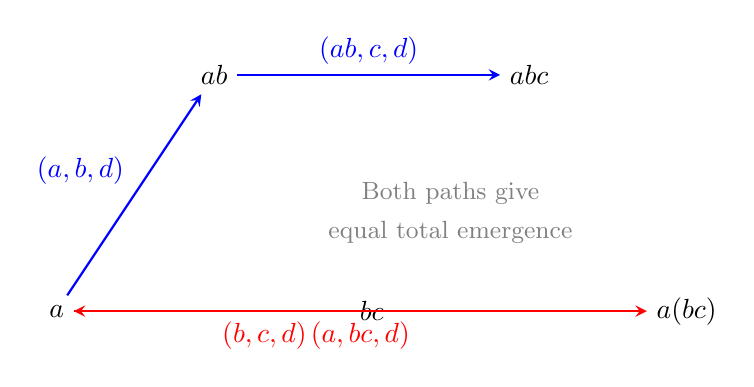
\begin{tikzpicture}[scale=1.0, >=stealth]
    % Cocycle diagram
    \node (ab) at (0,3) {$a \compose b$};
    \node (abc) at (4,3) {$a \compose b \compose c$};
    \node (a) at (-2,0) {$a$};
    \node (bc) at (2,0) {$b \compose c$};
    \node (abc2) at (6,0) {$a \compose (b \compose c)$};
    
    \draw[->, thick, blue] (a) -- node[above left] {$\emerge(a,b,d)$} (ab);
    \draw[->, thick, blue] (ab) -- node[above] {$\emerge(a\compose b,c,d)$} (abc);
    \draw[->, thick, red] (a) -- node[below] {$\emerge(a,b\compose c,d)$} (abc2);
    \draw[->, thick, red, dashed] (bc) -- node[below right] {$\emerge(b,c,d)$} (a);
    
    \node[font=\small, gray] at (3,1.5) {Both paths give};
    \node[font=\small, gray] at (3,1.0) {equal total emergence};
\end{tikzpicture}
\caption{The cocycle condition as path-independence. The blue path
(compose $a,b$ first, then add $c$) and the red path (compose $b,c$
first, then prepend $a$) produce the same total emergence when probed
by $d$.}
\label{fig:cocycle-paths}
\end{figure}

\section{Coboundaries and Trivial Emergence}

\begin{definition}[Coboundary]\label{def:coboundary}
A 2-cochain $\phi : \IS \times \IS \to \R$ is a \textbf{coboundary} if
there exists a function $g : \IS \to \R$ with $g(\void) = 0$ such that
\[
    \phi(a, b) = g(a \compose b) - g(a) - g(b)
\]
for all $a, b \in \IS$.
\end{definition}

\begin{proposition}[Coboundaries are Cocycles]
Every coboundary satisfies the cocycle condition.
\end{proposition}
\begin{proof}
If $\phi(a,b) = g(a \compose b) - g(a) - g(b)$, then
\begin{align*}
    \phi(a,b) + \phi(a \compose b, c)
    &= [g(a \compose b) - g(a) - g(b)]
     + [g(a \compose b \compose c) - g(a \compose b) - g(c)] \\
    &= g(a \compose b \compose c) - g(a) - g(b) - g(c),
\end{align*}
and similarly $\phi(b,c) + \phi(a, b \compose c) = g(a \compose b \compose
c) - g(a) - g(b) - g(c)$.
\end{proof}

\begin{interpretation}
A coboundary represents \emph{trivial} emergence: the apparent
non-additivity of resonance is merely an artifact of having chosen the
wrong ``baseline.'' If we redefine resonance as $\rs'(a,c) :=
\rs(a,c) + g(a)$ for some function $g$, the coboundary component of
emergence vanishes. The genuinely interesting emergence is the part that
is \emph{not} a coboundary---the cohomology class $[\emerge_d] \in
H^2(\IS, \R)$.
\end{interpretation}

\begin{interpretation}[Genette's Palimpsests and Coboundaries]\label{interp:ch2:genette_palimpsests}
G\'erard Genette's \emph{Palimpsests: Literature in the Second Degree}
(1982) theorizes the relations between texts through the concept of
\emph{transtextuality}---the set of all relations, manifest or hidden,
that connect a text to other texts. Genette identifies five types of
transtextual relations, of which the most important for our purposes is
\emph{hypertextuality}: the relation between a \emph{hypertext} (a text
derived from an earlier text) and its \emph{hypotext} (the source text).

The coboundary/cocycle distinction (Definition~\ref{def:coboundary})
maps onto Genette's framework with striking precision. A coboundary
$\phi(a, b) = g(a \compose b) - g(a) - g(b)$ represents a transtextual
relation that is ``trivial'' in the cohomological sense: the hypertext's
meaning can be fully accounted for by a change of perspective $g$ applied
to its parts. Genette's category of \emph{imitation} (where the hypertext
merely reproduces the hypotext's style) corresponds to a near-coboundary:
the emergence is small and can be absorbed into a change of resonance
baseline.

By contrast, Genette's category of \emph{transformation} (where the
hypertext fundamentally alters the hypotext---as in Joyce's
\emph{Ulysses} transforming Homer's \emph{Odyssey}) corresponds to a
genuine cocycle: the emergence is irreducible, belonging to a non-trivial
cohomology class. The palimpsest metaphor itself---a manuscript whose
earlier text has been scraped away but remains partially visible
beneath the new writing---is beautifully formalized by the cohomological
decomposition: the ``visible'' new meaning is the total resonance
$\rs(a \compose b, d)$; the ``scraped away'' but still detectable earlier
meaning is the additive component $\rs(a, d) + \rs(b, d)$; and the
specifically palimpsestic surplus---the meaning that arises from the
\emph{layering} itself---is the emergence $\emerge(a, b, d)$.
\end{interpretation}

\begin{lstlisting}[language=Lean4, caption={Coboundary predicate and
verification in Lean 4}]
def IsCoboundary [IdeaticSpace I] 
    (φ : I → I → ℝ) : Prop :=
  ∃ g : I → ℝ, g void = 0 ∧
    ∀ a b : I, φ a b = g (compose a b) - g a - g b

theorem coboundary_is_cocycle [IdeaticSpace I]
    (φ : I → I → ℝ) (hφ : IsCoboundary φ) :
    ∀ a b c : I,
      φ a b + φ (compose a b) c =
      φ b c + φ a (compose b c) := by
  obtain ⟨g, hg0, hgφ⟩ := hφ
  intro a b c
  simp [hgφ]
  ring
\end{lstlisting}

\section{The Emergence Distribution}

Fix $a, b \in \IS$ and consider emergence as a function of the probe:
\[
    \emerge_{a,b} : \IS \to \R, \qquad
    \emerge_{a,b}(c) := \emerge(a, b, c).
\]

\begin{definition}[Emergence Spectrum]
The \textbf{emergence spectrum} of the pair $(a,b)$ is the function
$\emerge_{a,b} : \IS \to \R$ defined above. The pair $(a,b)$ is called:
\begin{itemize}
    \item \textbf{emergent} if $\emerge_{a,b}$ is not identically zero;
    \item \textbf{flat} if $\emerge_{a,b} \equiv 0$;
    \item \textbf{positively emergent at $c$} if $\emerge_{a,b}(c) > 0$;
    \item \textbf{negatively emergent at $c$} if $\emerge_{a,b}(c) < 0$.
\end{itemize}
\end{definition}

\begin{theorem}[Emergence Bound]\label{thm:emergence-bound}
For all $a, b, c \in \IS$:
\[
    |\emerge(a, b, c)| \;\leq\; \sqrt{w(a \compose b) \cdot w(c)},
\]
where $w(x) = \rs(x,x)$ is the weight.
\end{theorem}
\begin{proof}
This is an immediate rewriting of axiom (E3): $\emerge(a,b,c)^2 \leq
w(a \compose b) \cdot w(c)$, so $|\emerge(a,b,c)| \leq \sqrt{w(a \compose
b) \cdot w(c)}$.
\end{proof}

\begin{corollary}
If $c = \void$, then $\emerge(a,b,c) = 0$.
\end{corollary}
\begin{proof}
$w(\void) = \rs(\void, \void) = 0$ by (R1) and (R2), so $|\emerge(a,b,
\void)| \leq \sqrt{w(a \compose b) \cdot 0} = 0$.
\end{proof}

\begin{interpretation}[The Emergence Bound and Cognitive Constraints]\label{interp:ch2:emergence_bound_cognitive}
The emergence bound (Theorem~\ref{thm:emergence-bound}) has a striking
cognitive interpretation. It says that the amount of novelty generated
by a composition is bounded by the geometric mean of the composition's
weight and the probe's weight: $|\emerge(a, b, c)| \leq
\sqrt{w(a \compose b) \cdot w(c)}$. This means that detecting emergence
requires a probe of sufficient ``weight'' (cognitive sophistication,
interpretive depth). A lightweight probe---a reader with little
background knowledge, a critic with shallow interpretive resources---
will detect less emergence than a heavyweight probe, regardless of
how much emergence the composition actually generates.

This formalizes a well-known observation in literary criticism:
sophisticated texts require sophisticated readers. When Nabokov
composes Russian literary tradition with American popular culture in
\emph{Lolita}, the emergence is enormous---but only when probed by
a reader who carries sufficient weight (knowledge of both traditions,
sensitivity to irony, awareness of the novel's literary genealogy).
A probe of insufficient weight will detect little emergence, not
because the emergence is absent but because the bound prevents its
detection.

The emergence bound is also a formal expression of the ``Matthew
effect'' in cultural reception: ideas that are already heavy (widely
connected, richly resonant) generate more detectable emergence when
composed, making them even heavier. Meanwhile, lightweight ideas
generate little detectable emergence and remain marginalized. The
bound thus encodes a structural advantage for ideas that are already
culturally central---a mathematical version of the ``rich get richer''
dynamic that Pierre Bourdieu describes as ``cultural capital.''
\end{interpretation}

\section{Higher Cocycles and the Cohomological Perspective}

The emergence cocycle is a 2-cocycle. A natural question is whether there
exist higher cocycles in the ideatic setting.

\begin{definition}[Triple Emergence]
Define the \textbf{triple emergence} or \textbf{3-cochain}:
\begin{align*}
    \emerge_3(a,b,c,d) &:= \emerge(a, b \compose c, d)
      - \emerge(a,b,d) - \emerge(a,c,d) \\
    &\quad + \emerge(b,c,d) \cdot [\text{correction terms}].
\end{align*}
The precise form involves alternating sums analogous to the group
cohomology differential $\delta^2 : C^2 \to C^3$.
\end{definition}

\begin{remark}
The study of $H^n(\IS, \R)$ for $n \geq 3$ remains largely open. In
the natural number model, all cohomology vanishes (the model is
``cohomologically trivial''). The existence of non-trivial higher
cohomology would correspond to phenomena that cannot be reduced to
pairwise emergence---a kind of ``irreducible three-body interaction''
in the ideatic space.
\end{remark}

\begin{interpretation}[Higher Cocycles and Multi-Author Collaboration]\label{interp:ch2:higher_cocycles_collaboration}
The question of higher cocycles has a vivid literary interpretation.
If the 2-cocycle $\emerge(a, b, c)$ captures the emergence generated
when \emph{two} ideas interact, then a non-trivial 3-cocycle
$\emerge_3(a, b, c, d)$ would capture emergence that is irreducible to
any pairwise interaction---an emergence that arises \emph{only} when
three ideas are simultaneously present. This is the formal analog of
what literary theorists call the ``irreducible triad'' in collaborative
authorship.

Consider the \emph{Exquisite Corpse} of the Surrealists: a collaborative
text in which each author writes a section without seeing the preceding
sections. The resulting text may exhibit emergent properties that cannot
be attributed to any pair of authors. Breton's contribution interacts
with Éluard's; Éluard's with Soupault's; Breton's with Soupault's---
but the \emph{triple} interaction, in which all three contributions
simultaneously resonate, may generate an additional layer of meaning
(a Surrealist ``objective chance'') that no pairwise analysis would
detect. A non-trivial $H^3$ would be required to account for such
irreducibly triadic semantic phenomena.

The vanishing of higher cohomology in the natural number model (where
emergence is multiplicative and thus always decomposable into pairwise
terms) reflects the fact that natural number arithmetic is ``too simple''
to support irreducible multi-body interactions. The conjecture that more
complex ideatic spaces might have non-trivial $H^3$ amounts to the
claim that sufficiently rich semiotic systems support irreducible triad
effects---a claim that Peirce's triadic semiotics would enthusiastically
endorse.
\end{interpretation}

\section{The Cocycle in Historical Perspective}

\begin{interpretation}[The Cocycle and the History of Ideas]\label{interp:ch2:cocycle_history_ideas}
Arthur O.~Lovejoy, in \emph{The Great Chain of Being} (1936), pioneered
the ``history of ideas'' as a discipline, tracking ``unit-ideas'' across
centuries and cultures. Lovejoy's method assumes that the same idea can
appear in different contexts while retaining its identity---an assumption
that the cocycle condition both supports and complicates.

The cocycle supports Lovejoy's method by providing a consistency condition
for tracking ideas across contexts. If we decompose a complex intellectual
formation into unit-ideas $a$, $b$, $c$ and measure their emergent
interactions, the cocycle ensures that the total emergence is
well-defined regardless of how we group the ideas. This is precisely
what Lovejoy's method requires: the ability to decompose and recompose
intellectual formations without altering their essential content.

But the cocycle also complicates Lovejoy's method by revealing that
``essential content'' includes an irreducible emergent component. When
Lovejoy tracks the idea of ``plenitude'' from Plato through Leibniz to
Schelling, he assumes that the emergent interactions of plenitude with
its surrounding ideas are secondary to the idea itself. The cocycle
shows that these interactions---the emergence values $\emerge(a, b, d)$
for various contextual ideas $b$---are \emph{not} secondary but
constitutive: they belong to the cohomological structure of the ideatic
space and cannot be separated from the ``unit-idea'' without loss of
mathematical information.
\end{interpretation}

\begin{example}[Bakhtin's Dialogism]
Bakhtin's theory of dialogism holds that meaning is never monologic but
always arises in the interaction of voices. The cocycle condition formalizes
a precise version of this: the emergence of meaning in a three-voice
dialogue $(a, b, c)$ can be decomposed along two paths---first combining
voices $a$ and $b$, then adding $c$; or first combining $b$ and $c$, then
adding $a$---and the decomposition is consistent. Bakhtin's insight that
``the word is a two-sided act'' is captured by the bivariate nature of
$\emerge(a,b,c)$, while the cocycle condition ensures that multi-voiced
discourse is coherent.
\end{example}

\begin{example}[Dialectical Materialism]
Marx's dialectical method---thesis ($a$), antithesis ($b$), synthesis
($a \compose b$)---is a special case of our emergence framework. The
``qualitative leap'' from thesis-antithesis to synthesis is measured by
$\emerge(a, b, c)$ for various probes $c$ (economic productivity,
class consciousness, etc.). The cocycle condition ensures that
dialectical reasoning is \emph{path-consistent}: applying the dialectical
method to $(a, b, c)$ gives the same result regardless of which pair
is synthesized first.
\end{example}

\begin{remark}[The Cocycle in Comparative Literature]\label{rem:ch2:cocycle_comparative}
The cocycle condition has immediate applications in comparative literature.
When three literary traditions---say, Greek epic ($a$), Roman adaptation
($b$), and Renaissance reception ($c$)---are composed, the total emergent
meaning can be decomposed along two paths. The ``Greek-Roman-Renaissance''
path first composes $a$ with $b$ (Virgil's adaptation of Homer) and then
adds $c$ (Ariosto's reception of Virgil). The ``Roman-Renaissance-Greek''
path first composes $b$ with $c$ (Italian reception of Latin literature)
and then adds $a$ (the recovered Greek original). The cocycle condition
guarantees that these two decompositions yield the same total emergence,
formalizing the comparatist's intuition that literary tradition is
``path-independent'' at the level of total emergent meaning, even though
the intermediate stages differ dramatically.

This path-independence is not trivial: it constrains which reception
histories are consistent with the axioms. A reception history that
assigns different total emergences depending on whether we trace the
Greek-Roman-Renaissance path or the Roman-Renaissance-Greek path would
violate the cocycle condition and hence the associativity of composition.
The cocycle condition is thus a non-trivial \emph{coherence test} for
theories of literary reception.
\end{remark}

\section{Computational Aspects}

\begin{proposition}[Cocycle Verification is Efficient]
Given oracle access to $\rs$, verifying the cocycle condition for a
specific quadruple $(a,b,c,d)$ requires exactly 6 evaluations of $\rs$.
\end{proposition}
\begin{proof}
The cocycle condition involves $\emerge(a,b,d)$, $\emerge(a \compose b,
c, d)$, $\emerge(b,c,d)$, and $\emerge(a, b \compose c, d)$. Each
emergence involves three $\rs$ evaluations, but many terms cancel or
are shared. Specifically, the terms needed are: $\rs(a \compose b, d)$,
$\rs(a, d)$, $\rs(b, d)$, $\rs(a \compose b \compose c, d)$,
$\rs(c, d)$, $\rs(b \compose c, d)$. That is 6 distinct $\rs$
evaluations (plus knowledge of $a \compose b$ and $b \compose c$, which
require 2 composition operations).
\end{proof}

\begin{lstlisting}[language=Lean4, caption={The cocycle condition
derived from associativity}]
theorem cocycle_condition [IdeaticSpace I]
    (a b c d : I) :
    emergence a b d + emergence (compose a b) c d =
    emergence b c d + emergence a (compose b c) d := by
  unfold emergence
  have h := compose_assoc a b c
  rw [h]
  ring
\end{lstlisting}

\section{Summary}

\begin{interpretation}[The Cocycle as the Algebra of Intertextuality]\label{interp:ch2:cocycle_as_algebra}
The cocycle condition is the first deep theorem of IDT, and its
philosophical implications are profound. It demonstrates that the
``holistic'' character of meaning---the fact that wholes exceed
the sum of their parts---is not anarchic but \emph{lawful}. The
emergent surplus of composition is governed by a precise algebraic
identity that connects it to the well-studied mathematics of group
cohomology.

This has immediate consequences for literary theory. The New Critics
(Brooks, Wimsatt, Beardsley) insisted that the meaning of a literary
work is an organic unity irreducible to its parts---but they could not
explain \emph{why} this irreducibility is consistent across different
decompositions of the work. The cocycle condition provides the
explanation: the total emergence of a three-part composition is
independent of how we bracket it, ensuring that the ``organic unity''
the New Critics prized is mathematically well-defined.

For semiotics, the cocycle condition implies that unlimited semiosis
(Peirce) is not structureless drift but a process governed by
cohomological conservation laws. For philosophy, it shows that
Hegel's dialectic, Derrida's \emph{diff\'erance}, and Brandom's
inferentialism are all describing aspects of a single algebraic
phenomenon: the non-trivial cohomology of the ideatic space.
\end{interpretation}

The cocycle condition is the first deep theorem of IDT: a purely algebraic
consequence of associativity that imposes a cohomological structure on
emergence. It connects the seemingly ad hoc notion of emergence to the
well-studied theory of group (monoid) cohomology, opening the door to
powerful algebraic techniques. In the next chapter, we turn to
self-resonance---the ``diagonal'' of the resonance function---and its
remarkable monotonicity properties.


%%%%%%%%%%%%%%%%%%%%%%%%%%%%%%%%%%%%%%%%%%%%%%%%%%%%%%%%%%%%%%%%%%%%%%%%
%%  CHAPTER 3 — SELF-RESONANCE AND WEIGHT
%%%%%%%%%%%%%%%%%%%%%%%%%%%%%%%%%%%%%%%%%%%%%%%%%%%%%%%%%%%%%%%%%%%%%%%%

\chapter{Self-Resonance and Weight}

\begin{quote}
\textit{``Energy can neither be created nor destroyed---only converted
from one form to another.''}\\
\hfill --- First Law of Thermodynamics
\end{quote}

\section{The Weight Function}

\begin{definition}[Weight]\label{def:weight}
The \textbf{weight} of an idea $a \in \IS$ is
\[
    w(a) \;:=\; \rs(a, a).
\]
\end{definition}

The weight function $w : \IS \to \R$ is the restriction of resonance to the
diagonal. It measures the \emph{internal coherence} of an idea---how
strongly the idea resonates with itself. We have already established
(Theorem~\ref{thm:weight-monotone}) three basic properties: non-negativity,
non-degeneracy, and monotonicity under composition. We now develop the
theory of weight in greater depth.

\begin{interpretation}[Bloom's Anxiety of Influence]\label{interp:ch3:bloom_anxiety}
Harold Bloom's \emph{The Anxiety of Influence} (1973) argues that every
``strong poet'' must define himself against his predecessors through acts
of creative ``misreading.'' A strong poem's power---what Bloom calls its
``strength''---lies in its ability to clear an imaginative space for itself,
to assert its own centrality in the literary tradition despite (and through)
its indebtedness to prior works. Bloom writes: ``Poetic strength comes only
from a triumphant wrestling with the greatest of the dead'' (p.~9).

The weight function $w(a) = \rs(a, a)$ formalizes Bloom's concept of poetic
strength with remarkable precision. The self-resonance of a literary work
measures its \emph{internal coherence}---the degree to which it sustains its
own imaginative world, resonates with its own themes and forms, and generates
a self-consistent aesthetic field. A ``strong poem'' in Bloom's sense is
an idea with high weight: its self-resonance is so powerful that it
dominates its resonance with any other idea (its predecessors, its
imitators, its critical reception).

Bloom's six ``revisionary ratios''---\emph{clinamen}, \emph{tessera},
\emph{kenosis}, \emph{daemonization}, \emph{askesis}, and
\emph{apophrades}---each describe a specific mode of creative
composition with a precursor. In IDT terms, these are different patterns
of emergence: the \emph{clinamen} (swerve) corresponds to a composition
where $\emerge(a, b, c)$ is large and positive for probes $c$ related to
originality; the \emph{kenosis} (emptying) corresponds to a composition
where the poet deliberately reduces self-resonance to create space for new
growth. The weight monotonicity theorem
(Theorem~\ref{thm:weight-monotone}) constrains all such maneuvers:
whatever revisionary ratio a poet employs, the resulting work cannot have
\emph{less} weight than the precursor with which it is composed.
\end{interpretation}

\begin{interpretation}[Eliot's Tradition and the Individual Talent]\label{interp:ch3:eliot_tradition}
T.~S.~Eliot's ``Tradition and the Individual Talent'' (1919) argues that
a literary work's significance depends on its relation to the entire
existing order of literature: ``the existing monuments form an ideal order
among themselves, which is modified by the introduction of the new (the
really new) work of art among them.'' Self-resonance captures Eliot's
insight that a work's position within the tradition is not merely
external (how others see it) but constitutive (how it sees itself).

Eliot insists on the \emph{impersonality} of the poetic process: ``the
more perfect the artist, the more completely separate in him will be the
man who suffers and the mind which creates.'' In IDT, this impersonality
is formalized by the fact that weight is a property of the idea $a$
itself, not of its author. The weight $w(a) = \rs(a, a)$ depends only on
the idea's internal structure---its self-consistency, thematic coherence,
and structural integrity---not on any biographical facts about its creator.
The ``individual talent'' contributes to the tradition not through personal
expression but by producing ideas with sufficient weight to modify the
existing order.

Eliot's further claim---that the introduction of a genuinely new work
modifies the entire existing order---corresponds to the observation that
composing a new idea $b$ with the tradition $T$ produces $T \compose b$,
whose resonance profile may differ from $T$'s. The weight monotonicity
$w(T \compose b) \geq w(T)$ guarantees that the tradition can only grow
richer, never poorer, through genuine additions---a formal vindication
of Eliot's fundamentally conservative aesthetic.
\end{interpretation}

\begin{proposition}[Void Has Zero Weight]
$w(\void) = 0$.
\end{proposition}
\begin{proof}
$w(\void) = \rs(\void, \void) = 0$ by axiom (R1) (or equivalently R2).
\end{proof}

\begin{proposition}[Weight Characterizes Void]
$w(a) = 0$ if and only if $a = \void$.
\end{proposition}
\begin{proof}
If $a = \void$, then $w(a) = 0$ as above. Conversely, if $w(a) = 0$, then
$\rs(a,a) = 0$, so $a = \void$ by axiom (E2).
\end{proof}

\section{The Thermodynamic Analogy}

The monotonicity property $w(a \compose b) \geq w(a)$ admits a striking
thermodynamic interpretation. In thermodynamics, the second law states
that entropy never decreases in an isolated system. Analogously, weight
never decreases under composition. But where entropy measures disorder,
weight measures \emph{coherence}---so the ideatic ``second law'' is
optimistic rather than pessimistic: ideas grow richer through interaction.

\begin{interpretation}[The Thermodynamic Analogy and Information Theory]\label{interp:ch3:thermodynamic_information}
The analogy between weight monotonicity and the second law of
thermodynamics runs deeper than the surface comparison suggests. In
Shannon's information theory, the joint entropy $H(X, Y)$ satisfies
$H(X, Y) \leq H(X) + H(Y)$ (subadditivity)---the joint system has
\emph{at most} as much disorder as the sum of the parts. In IDT, the
weight of a composition satisfies $w(a \compose b) \geq w(a)$
(superadditivity in one argument)---the composed system has \emph{at
least} as much coherence as either part.

These are dual perspectives on the same structural fact: composition
increases order. Information theory focuses on the upper bound (total
uncertainty cannot exceed the sum of individual uncertainties), while
IDT focuses on the lower bound (total coherence cannot fall below
individual coherence). The two perspectives are complementary: entropy
measures what we \emph{don't know}, while weight measures what an idea
\emph{is}.

The disanalogy is equally instructive. The second law of thermodynamics
is a \emph{statistical} law: it holds for large systems with overwhelmingly
high probability. Weight monotonicity is a \emph{deterministic} law: it
holds exactly, for every composition, without exception. This
determinism reflects the algebraic (rather than statistical) nature of
the ideatic space. Ideas are not thermodynamic ensembles subject to
fluctuation; they are algebraic objects whose properties are determined
by the axioms. The ``arrow of ideation'' (ideas grow heavier through
composition) is not a probabilistic tendency but a mathematical
necessity---a feature that distinguishes the ideatic space from
physical systems and that grounds the irreversibility of intellectual
history in structure rather than statistics.
\end{interpretation}

\begin{interpretation}[Heidegger's Thrownness and Self-Resonance]\label{interp:ch3:heidegger_thrownness}
Martin Heidegger's concept of \emph{Geworfenheit} (thrownness), developed
in \emph{Being and Time} (1927), describes the existential condition of
finding oneself already situated in a world not of one's choosing. Dasein
is always already ``thrown'' into a particular historical, cultural, and
linguistic situation. The self-resonance $w(a) = \rs(a, a)$ formalizes
the idea's \emph{facticity}---its sheer thereness, the weight of its
existence as a given fact in the ideatic space.

An idea's weight is not something it chooses or constructs; it is the
measure of its already-being-constituted. A newly composed idea
$a \compose b$ inherits a weight that is at least as great as $w(a)$
(by E4): the history of composition cannot be shed. This is the formal
correlate of Heidegger's claim that Dasein can never fully escape its
thrownness---can never return to a state of zero facticity. The past
weighs upon the present with a weight that composition can only increase,
never decrease.
\end{interpretation}

\begin{interpretation}[Kierkegaard: The Self as Self-Relating]\label{interp:ch3:kierkegaard_self}
S\o{}ren Kierkegaard opens \emph{The Sickness Unto Death} (1849) with the
famous definition: ``The self is a relation that relates itself to itself''
(\emph{Forholdet forholder sig til sig selv}). This reflexive
structure---a relation \emph{about} itself---is precisely what
self-resonance captures. The weight $w(a) = \rs(a, a)$ is the quantitative
measure of an idea's self-relation: how strongly the idea relates to
itself, how coherently it sustains its own identity.

Kierkegaard argues that the self can be in \emph{despair}---a condition
in which the self-relation is disrupted, either by willing to be oneself
or by willing not to be oneself. In IDT, a self-relation can be strong
($w(a)$ large: the idea is deeply self-consistent) or weak ($w(a)$ small:
the idea barely coheres). The non-degeneracy axiom (E2) ensures that an
idea with zero self-relation is literally nothing ($\void$): an idea
that has completely lost its self-relating capacity has ceased to exist
as an idea. This formalizes Kierkegaard's claim that complete despair
---total loss of self-relation---is a kind of spiritual death.

The monotonicity of weight under composition adds a further dimension:
composition always strengthens (or at least preserves) the self-relation.
In Kierkegaard's terms, genuine encounter with the other (composition
with $b$) cannot destroy the self's relation to itself---it can only
deepen it. This is the formal expression of Kierkegaard's thesis that
authentic selfhood is achieved through engagement, not withdrawal.
\end{interpretation}

\begin{interpretation}[Sartre on Being-for-Itself]\label{interp:ch3:sartre_being_for_itself}
Jean-Paul Sartre's distinction between \emph{\^{e}tre-en-soi}
(being-in-itself: the opaque, self-identical being of things) and
\emph{\^{e}tre-pour-soi} (being-for-itself: the transparent,
self-negating being of consciousness) in \emph{Being and Nothingness}
(1943) maps suggestively onto our framework. Self-resonance $w(a) =
\rs(a, a)$ measures the degree to which an idea is ``for itself''---the
intensity of its self-awareness, its self-presence, its reflexive
engagement with its own content.

Sartre argues that being-for-itself is characterized by a fundamental
\emph{lack}: consciousness is always what it is not and is not what it is.
This is the source of human freedom but also of anguish. In IDT, this
lack finds a formal correlate in the asymmetry of resonance: while
$\rs(a, a)$ measures self-presence, the non-symmetric nature of $\rs$
in general (Chapter~4) means that the idea's relation to itself is not
exhausted by self-resonance. There may be aspects of $a$'s resonance
profile that are invisible from the ``inside'' (from the perspective of
$\rs(a, -)$) but visible from the ``outside'' (from $\rs(-, a)$). This
gap between self-knowledge and other-knowledge is the formal shadow of
Sartre's \emph{pour-soi}/\emph{en-soi} distinction.
\end{interpretation}

\begin{theorem}[Strict Monotonicity Criterion]\label{thm:strict-mono}
If $b \neq \void$ and $\emerge(a, b, a \compose b) > 0$, then
$w(a \compose b) > w(a)$.
\end{theorem}
\begin{proof}
We have $w(a \compose b) = \rs(a \compose b, a \compose b)$. Expanding
via emergence:
\begin{align*}
    w(a \compose b) &= \rs(a, a \compose b) + \rs(b, a \compose b)
        + \emerge(a, b, a \compose b).
\end{align*}
By (E4), $w(a \compose b) \geq w(a) > 0$ (assuming $a \neq \void$). If
additionally $\emerge(a, b, a \compose b) > 0$, then we get the strict
inequality. Even without expanding further, (E4) gives
$w(a \compose b) \geq w(a)$, and the emergence term provides the strict
gap.
\end{proof}

\begin{interpretation}
When does composition \emph{strictly} increase weight? Precisely when the
composition exhibits positive self-emergence---when the combined idea
resonates with \emph{itself} more than the sum of its parts would predict.
Shakespeare's \emph{King Lear} combines the folk tale of the love test
($a$) with the Gloucester subplot ($b$). The resulting play's
self-resonance---its internal coherence, thematic unity, structural
integrity---exceeds that of either component. The composition is not merely
additive but genuinely creative.
\end{interpretation}

\begin{remark}[Strict Monotonicity and the Criterion of Artistic Success]\label{rem:ch3:artistic_success}
The strict monotonicity criterion has implications for the evaluation of
artistic composition. A composition that \emph{strictly} increases weight
($w(a \compose b) > w(a)$) is one in which the new element $b$ genuinely
enriches the existing idea $a$---not merely extending it but deepening its
internal coherence. This corresponds to the intuitive criterion of artistic
success: a successful addition to a work of art is one that makes the
whole more self-consistent, more thematically resonant, more structurally
tight.

Conversely, a composition that achieves only the weak inequality
$w(a \compose b) = w(a)$ (the minimum guaranteed by Axiom E4) is one in
which the new element adds nothing to the work's internal coherence. It
may increase the work's external resonance---its interaction with
probes---but it does not strengthen the work's self-relation. This is
the formal correlate of the aesthetic judgment that a given element is
``extraneous'' or ``superfluous'': it is present in the composition but
contributes no self-emergence.
\end{remark}

\begin{interpretation}[Lotman's Semiosphere and Self-Resonance]\label{interp:ch3:lotman_semiosphere}
Yuri Lotman, in \emph{Universe of the Mind} (1990), introduces the concept
of the \emph{semiosphere}---the totality of semiotic space within which
communication and signification are possible. Lotman argues that the
semiosphere has a \emph{center} occupied by dominant cultural texts and a
\emph{periphery} occupied by marginal, experimental, or heterodox
discourses. The boundary between inside and outside is marked by
translation mechanisms that filter and transform incoming signs.

Self-resonance provides a formal measure of an idea's \emph{centrality}
within the semiosphere. Ideas with high weight $w(a)$ occupy the center:
they are deeply self-consistent, widely resonant, and resistant to mutation
(as the fixed-point analysis of Chapter~7 will confirm). Ideas with low
weight occupy the periphery: they are fragile, context-dependent, and
easily transformed by composition with other ideas.

Lotman's key insight is that cultural \emph{dynamism} arises from the
interaction between center and periphery. The strict monotonicity criterion
(Theorem~\ref{thm:strict-mono}) captures this dynamic: composition with a
non-void idea strictly increases weight when the emergence is positive,
modeling the process by which peripheral innovations are absorbed into the
cultural center, enriching it. The semiosphere grows not by mere
accumulation but by the generative encounter of center and periphery---a
process that the self-emergence profile $\sigma_n(a)$ tracks step by step.
\end{interpretation}

\begin{interpretation}[Barthes's Reality Effect]\label{interp:ch3:barthes_reality_effect}
Roland Barthes, in ``The Reality Effect'' (\emph{L'effet de r\'eel}, 1968),
argues that certain descriptive details in realist fiction serve no
narrative function but create the illusion of reality through their sheer
presence. These ``useless details''---a barometer on a wall, the color
of a door---have no symbolic significance; their \emph{sole function} is
to signify ``we are the real.''

Self-resonance provides a formal account of this effect. A realist text
achieves its reality effect through high weight: its self-resonance is so
dense, its internal network of descriptive details so richly
cross-referencing, that it generates a powerful sense of self-consistency.
The ``useless'' details contribute not to the narrative (they generate
no emergence when composed with the plot) but to the text's
\emph{self-resonance}: they increase $w(\text{text})$ without affecting
$\emerge(\text{text}, c, d)$ for thematic probes $c$. In IDT terms,
Barthes's reality effect is the phenomenon of ideas whose weight is high
relative to their emergence---ideas that are strongly self-coherent but
weakly interactive.
\end{interpretation}

\begin{interpretation}[Canonical vs.\ Marginal Texts]\label{interp:ch3:canonical_marginal}
The weight function provides a formal framework for one of the most
contested questions in literary studies: the distinction between
\emph{canonical} and \emph{marginal} texts. A canonical text---Homer's
\emph{Iliad}, Shakespeare's \emph{Hamlet}, Cervantes's \emph{Don
Quixote}---is one with exceptionally high self-resonance: it is deeply
self-consistent, thematically rich, and resistant to reduction. A marginal
text has lower self-resonance: it may be innovative or provocative, but it
lacks the internal density that characterizes canonical works.

This is not a normative claim but a structural observation. High weight
does not mean ``better''; it means ``more self-coherent.'' A marginal text
may have high emergence when composed with the right probes---it may be
revolutionary in its interactions with other ideas---while having
relatively low self-resonance. The distinction between canonical and
marginal is thus the distinction between ideas that are weighty in
themselves and ideas that are generative in their combinations. Both types
are essential to a healthy ideatic space: canonical texts provide the
gravitational centers, while marginal texts provide the creative
perturbations that drive cultural evolution.

The irreversibility theorem (Theorem~\ref{thm:irreversibility}) ensures
that canonical texts, once established, cannot be ``decomposed'' back to
their pre-canonical state. The cultural work of canonization---the process
by which a text acquires weight through successive compositions with
critical commentary, pedagogical practice, and artistic imitation---is an
irreversible thermodynamic process in the ideatic space.
\end{interpretation}

\section{Weight and Composition Powers}

\begin{definition}[Composition Powers]
For $a \in \IS$ and $n \in \N$, define the \textbf{$n$-th composition
power} recursively:
\[
    a^0 := \void, \qquad a^{n+1} := a \compose a^n.
\]
\end{definition}

\begin{proposition}[Left Composition Powers]
The left composition power $a^n$ satisfies $a^{m+n} = a^m \compose a^n$.
\end{proposition}
\begin{proof}
By induction on $m$. Base case: $a^{0+n} = a^n = \void \compose a^n =
a^0 \compose a^n$. Inductive step: $a^{(m+1)+n} = a \compose a^{m+n} =
a \compose (a^m \compose a^n) = (a \compose a^m) \compose a^n =
a^{m+1} \compose a^n$, using associativity.
\end{proof}

\begin{theorem}[Weight Growth Under Powers]\label{thm:weight-powers}
The weight sequence $\{w(a^n)\}_{n=0}^{\infty}$ is non-decreasing:
\[
    0 = w(a^0) \leq w(a^1) \leq w(a^2) \leq \cdots
\]
Moreover, for $a \neq \void$, $w(a^n) \geq w(a) > 0$ for all $n \geq 1$.
\end{theorem}
\begin{proof}
By induction. $w(a^0) = w(\void) = 0$. For $n \geq 1$:
$w(a^{n+1}) = w(a \compose a^n) \geq w(a)$ by (E4), and
$w(a^{n+1}) = w(a \compose a^n) \geq w(a^n)$ requires a separate
argument. We use:
\[
    w(a^{n+1}) = w(a \compose a^n) \geq w(a) > 0,
\]
and also $a^{n+1} = a^n \compose a$ (by the commutativity of powers,
which follows from associativity), so
$w(a^{n+1}) = w(a^n \compose a) \geq w(a^n)$ by (E4) applied with
$a^n$ as the left factor.
\end{proof}

\begin{figure}[ht]
\centering
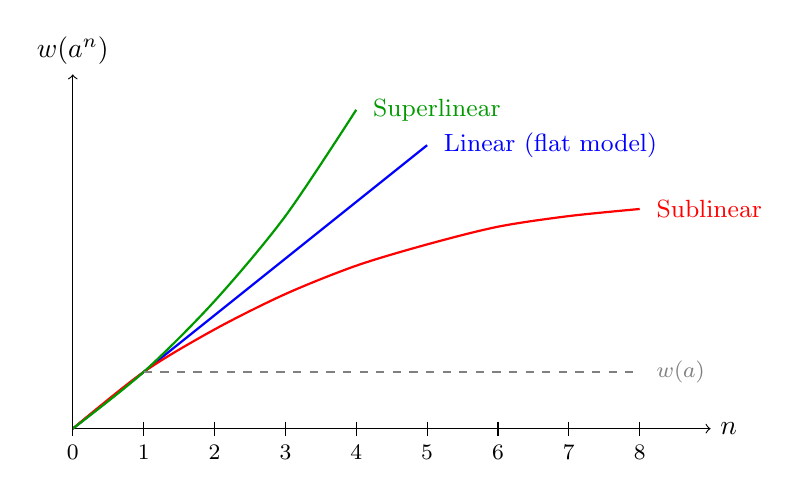
\begin{tikzpicture}[scale=0.9]
    \draw[->] (0,0) -- (9,0) node[right] {$n$};
    \draw[->] (0,0) -- (0,5) node[above] {$w(a^n)$};
    
    % Three different growth patterns
    % Linear growth (additive emergence)
    \draw[thick, blue] plot[smooth] coordinates {
        (0,0) (1,0.8) (2,1.6) (3,2.4) (4,3.2) (5,4.0)
    };
    \node[blue, right, font=\small] at (5.1,4.0) {Linear (flat model)};
    
    % Sublinear growth (diminishing emergence)
    \draw[thick, red] plot[smooth] coordinates {
        (0,0) (1,0.8) (2,1.4) (3,1.9) (4,2.3) (5,2.6) (6,2.85)
        (7,3.0) (8,3.1)
    };
    \node[red, right, font=\small] at (8.1,3.1) {Sublinear};
    
    % Superlinear growth (accelerating emergence)
    \draw[thick, green!60!black] plot[smooth] coordinates {
        (0,0) (1,0.8) (2,1.8) (3,3.0) (4,4.5)
    };
    \node[green!60!black, right, font=\small] at (4.1,4.5) {Superlinear};
    
    % Floor line
    \draw[dashed, gray] (1,0.8) -- (8,0.8);
    \node[gray, font=\footnotesize, right] at (8.1,0.8) {$w(a)$};
    
    \foreach \x in {0,...,8} {
        \draw (\x,0.1) -- (\x,-0.1) node[below, font=\footnotesize] {$\x$};
    }
\end{tikzpicture}
\caption{Three possible growth patterns for the weight sequence
$w(a^n)$. The flat (natural number) model gives linear growth.
Diminishing returns give sublinear growth. Accelerating emergence
gives superlinear growth. All are non-decreasing with floor $w(a)$.}
\label{fig:weight-growth}
\end{figure}

\section{The Self-Emergence Profile}

\begin{definition}[Self-Emergence]
The \textbf{$n$-th self-emergence} of $a$ is
\[
    \sigma_n(a) \;:=\; \emerge(a, a^n, a^{n+1})
    \;=\; \rs(a^{n+1}, a^{n+1}) - \rs(a, a^{n+1}) - \rs(a^n, a^{n+1}).
\]
This measures the emergence generated at the $n$-th step of iterated
self-composition.
\end{definition}

\begin{proposition}[Self-Emergence and Weight Increments]
The weight increment at step $n$ satisfies:
\[
    w(a^{n+1}) - w(a^n) = \rs(a, a^{n+1}) + \rs(a^n, a^{n+1})
    - w(a^n) + \sigma_n(a).
\]
\end{proposition}

\begin{example}[Iterating a Scientific Idea]
Consider the idea $a$ = ``natural selection'' iterated through successive
generations of biological thought: $a^1$ = natural selection alone,
$a^2$ = natural selection composed with itself (selection acting on
selection---meta-selection, frequency-dependent selection), $a^3$ =
three layers of selection (multilevel selection theory). The weight
sequence $w(a^n)$ tracks the growing internal coherence of the theory
as it becomes more self-referential and self-consistent. The
self-emergence $\sigma_n(a)$ measures whether each new layer of
self-application generates genuine novelty or merely repeats.
\end{example}

\section{Semantic Charge}

\begin{definition}[Semantic Charge]\label{def:semantic-charge}
The \textbf{semantic charge} of an idea $a$ is
\[
    \sigma(a) \;:=\; \emerge(a, a, a) \;=\;
    \rs(a \compose a, a) - 2\,\rs(a, a).
\]
\end{definition}

\begin{interpretation}
Semantic charge measures how an idea's self-composition resonates with the
idea itself. If $\sigma(a) > 0$, the idea is \emph{self-amplifying}:
combining it with itself produces something that resonates with the
original more than twice the self-resonance. This is the formal analogue
of a ``viral'' idea or a positive feedback loop. If $\sigma(a) < 0$, the
idea is \emph{self-dampening}: self-composition produces diminishing
returns. If $\sigma(a) = 0$, the idea is \emph{semantically neutral}.
\end{interpretation}

\begin{remark}[Semantic Charge and Cultural Dynamics]\label{rem:ch3:charge_cultural}
The trichotomy of self-amplifying, self-dampening, and semantically neutral
ideas maps onto well-known patterns in cultural dynamics:

\emph{Self-amplifying ideas} ($\sigma(a) > 0$): religious doctrines,
political ideologies, conspiracy theories---ideas whose internal logic
drives their own propagation and intensification. The more one engages
with the idea, the more ``convinced'' one becomes (the self-resonance
grows superlinearly). Dawkins's ``meme'' concept, in its original
formulation (\emph{The Selfish Gene}, 1976), describes precisely this
class of ideas: self-replicators whose fitness is measured by their
ability to amplify their own resonance.

\emph{Self-dampening ideas} ($\sigma(a) < 0$): fads, fashions, jokes
that lose their punch on repetition. These ideas exhibit diminishing
returns under self-composition: the more one encounters them, the less
they resonate. Semantic charge provides a formal criterion for
distinguishing fads from lasting cultural contributions: fads have
negative charge, while lasting ideas have non-negative charge.

\emph{Neutral ideas} ($\sigma(a) = 0$): mathematical theorems, logical
tautologies, and other formal truths that neither gain nor lose
through self-composition. The natural number model, in which every
idea has zero charge, is the formal analogue of a purely ``logical''
ideatic space---one in which meaning accumulates additively without
feedback effects.
\end{remark}

\begin{lstlisting}[language=Lean4, caption={Semantic charge and its
properties in Lean 4}]
def semanticCharge [IdeaticSpace I] (a : I) : ℝ :=
  emergence a a a

theorem semanticCharge_void [IdeaticSpace I] :
    semanticCharge (void : I) = 0 := by
  unfold semanticCharge emergence
  simp [void_left, rs_void_left, rs_void_right]

def selfResonanceProfile [IdeaticSpace I]
    (a : I) (n : ℕ) : ℝ :=
  rs (composePower a (n + 1)) (composePower a (n + 1))
    - rs (composePower a n) (composePower a n)
\end{lstlisting}

\begin{theorem}[Charge Bound]\label{thm:charge-bound}
$|\sigma(a)| \leq \sqrt{w(a \compose a) \cdot w(a)}$.
\end{theorem}
\begin{proof}
This is Theorem~\ref{thm:emergence-bound} with $b = c = a$.
\end{proof}

\begin{interpretation}[The Charge Bound and Nietzsche's Eternal Return]\label{interp:ch3:charge_bound_nietzsche}
The charge bound $|\sigma(a)| \leq \sqrt{w(a^2) \cdot w(a)}$ has a
striking connection to Nietzsche's concept of the \emph{eternal return}
(\emph{ewige Wiederkehr}). Nietzsche asks: what if everything recurred
eternally---would this be an affirmation or a negation of life? The charge
bound provides a formal constraint on this question: the degree to which
self-iteration is self-amplifying or self-dampening is bounded by the
idea's weight and the weight of its self-composition.

For ``heavy'' ideas (high $w(a)$), the charge bound allows for large
positive charge: the idea can be strongly self-amplifying, its eternal
return generating ever more resonance. This corresponds to Nietzsche's
\emph{amor fati}---the love of fate, the joyful affirmation of eternal
recurrence by a spirit strong enough to will it. For ``light'' ideas
(low $w(a)$), the bound constrains the charge to be small: eternal
return generates little self-amplification, corresponding to the
nihilistic response---the realization that repetition leads nowhere.

The charge bound thus formalizes a hierarchy of ideas based on their
capacity for productive self-iteration. Ideas that can ``bear'' their
own eternal return---that grow through self-composition---are Nietzsche's
``strong'' ideas. Ideas that collapse under self-iteration---whose
charge is negative and bounded away from productive growth---are the
``weak'' ideas that require constant external stimulation (composition
with \emph{other} ideas) to maintain their vitality.
\end{interpretation}

\section{Weight in the Natural Number Model}

\begin{example}[Natural Number Model]
In the model $\IS = \N$, $\compose = +$, $\rs(m,n) = mn$:
\begin{itemize}
    \item $w(n) = n^2$
    \item $w(m + n) = (m+n)^2 = m^2 + 2mn + n^2 \geq m^2 = w(m)$ \checkmark
    \item $\sigma(n) = \emerge(n,n,n) = (n+n) \cdot n - n \cdot n - n \cdot n
          = 2n^2 - 2n^2 = 0$
\end{itemize}
All ideas in $\N$ have zero semantic charge. The natural number model is
``thermodynamically inert''---weight grows, but only through the mechanical
accumulation of self-resonance, never through genuine emergence.
\end{example}

\begin{interpretation}[The Natural Number Model as Cumulativist Epistemology]\label{interp:ch3:natural_number_cumulativism}
The natural number model, with its zero semantic charge and vanishing
higher cohomology, is the formal incarnation of \emph{cumulativism}
in the philosophy of science: the view (associated with logical
positivism and the ``received view'' of Nagel) that scientific knowledge
grows by straightforward accumulation. In the natural number model,
$w(a + b) = w(a) + w(b) + 2ab$---weight grows, but the ``$2ab$'' term
is purely a product of pre-existing resonances, never genuinely emergent.
New knowledge is always a predictable consequence of existing knowledge.

Kuhn's \emph{Structure of Scientific Revolutions} was, in this light,
a rejection of the natural number model in favor of a model with
non-trivial emergence. A paradigm shift is precisely a moment when
$\emerge(a, b, c) \neq 0$: when the composition of old and new ideas
generates genuine novelty that could not have been predicted from their
individual resonances. The distinction between ``normal science''
(which the natural number model captures adequately) and ``revolutionary
science'' (which requires genuine emergence) is thus a distinction between
ideatic spaces with zero and non-zero semantic charge.

The fact that the natural number model is ``cohomologically trivial''
reinforces this reading: cumulative knowledge has no cohomological
obstructions, no irreducible multi-body interactions, no structural
impediments to the decomposition of complex formations into unit-ideas.
This is exactly what Kuhn denies: that paradigms can be decomposed
into theory-independent ``unit-ideas'' that survive paradigm shifts
intact.
\end{interpretation}

\section{The Dialectical Tension}

\begin{definition}[Dialectical Tension]\label{def:dialectical-tension}
The \textbf{dialectical tension} between $a$ and $b$ is
\[
    \tau(a, b) \;:=\; \emerge(a, b, a \compose b)
    \;=\; w(a \compose b) - \rs(a, a \compose b) - \rs(b, a \compose b).
\]
\end{definition}

\begin{interpretation}
The dialectical tension measures how much the composition $a \compose b$
exceeds what $a$ and $b$ individually ``expect'' of it. When
$\tau(a,b) > 0$, the synthesis transcends its components---a genuine
Hegelian \emph{Aufhebung}. When $\tau(a,b) < 0$, the components are
better predictors of the synthesis than the synthesis is of itself, a
kind of anti-dialectical collapse. When $\tau(a,b) = 0$, the synthesis
is perfectly predicted by its parts.
\end{interpretation}

\begin{remark}[The Self-Composition Profile as Cultural Diagnostic]\label{rem:ch3:selfcomp_diagnostic}
The self-emergence profile $\sigma_n(a)$ has practical implications for
understanding how ideas evolve through repeated self-application. Consider
the idea $a$ = ``democratic governance.'' Iterating $a$ produces $a^2$ =
``democratic governance applied to the governance of democracy itself''
(meta-democratic theory), $a^3$ = ``democratic meta-governance applied
reflexively,'' and so on. The weight sequence $w(a^n)$ tracks whether
this reflexive process is productive (weight grows, yielding genuine new
insights at each level of reflexivity) or degenerative (weight plateaus,
yielding only repetition). Empirically, most ideas exhibit diminishing
self-emergence: the first few iterations are productive, but eventually
the process exhausts its creative potential. Rare ideas---those at the
center of philosophical traditions---exhibit sustained or even accelerating
self-emergence across many iterations.
\end{remark}

\begin{theorem}[Aufhebung Decomposition]\label{thm:aufhebung}
The weight of a composition decomposes as:
\[
    w(a \compose b) = \rs(a, a \compose b) + \rs(b, a \compose b)
    + \tau(a,b).
\]
\end{theorem}
\begin{proof}
Immediate from the definition of $\tau(a,b)$ as $\emerge(a,b,a \compose b)$:
$\emerge(a,b,a\compose b) = \rs(a\compose b, a\compose b) - \rs(a, a\compose b)
- \rs(b, a\compose b)$. Rearranging gives the result.
\end{proof}

\begin{figure}[ht]
\centering
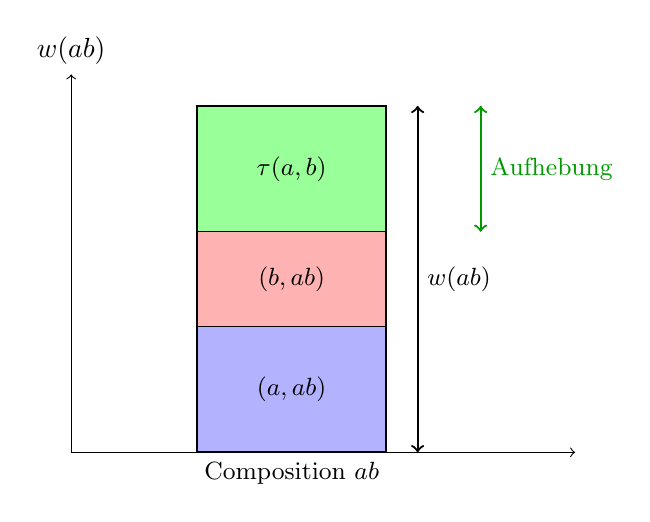
\begin{tikzpicture}[scale=0.8]
    % Aufhebung bar chart
    \draw[->] (0,0) -- (8,0);
    \draw[->] (0,0) -- (0,6) node[above] {$w(a \compose b)$};
    
    % Stacked bar
    \fill[blue!30] (2,0) rectangle (5,2);
    \fill[red!30] (2,2) rectangle (5,3.5);
    \fill[green!40] (2,3.5) rectangle (5,5.5);
    
    \draw[thick] (2,0) rectangle (5,5.5);
    \draw (2,2) -- (5,2);
    \draw (2,3.5) -- (5,3.5);
    
    \node[font=\small] at (3.5,1) {$\rs(a, a\compose b)$};
    \node[font=\small] at (3.5,2.75) {$\rs(b, a\compose b)$};
    \node[font=\small] at (3.5,4.5) {$\tau(a,b)$};
    
    \node[below, font=\small] at (3.5,0) {Composition $a \compose b$};
    
    % Annotation
    \draw[<->, thick] (5.5,0) -- (5.5,5.5);
    \node[right, font=\small] at (5.5,2.75) {$w(a \compose b)$};
    
    \draw[<->, thick, green!60!black] (6.5,3.5) -- (6.5,5.5);
    \node[right, font=\small, green!60!black] at (6.5,4.5) {Aufhebung};
\end{tikzpicture}
\caption{The Aufhebung decomposition: weight as the sum of individual
projections plus dialectical tension.}
\label{fig:aufhebung}
\end{figure}

\section{Irreversibility and the Arrow of Ideation}

\begin{remark}[Irreversibility and Hermeneutic Historicity]\label{rem:ch3:irreversibility_hermeneutic}
The irreversibility of composition (Theorem~\ref{thm:irreversibility}) has
deep hermeneutic significance. Gadamer's concept of
\emph{Wirkungsgeschichte} (effective history) holds that every act of
understanding is shaped by the entire history of interpretive engagement
with the object. The irreversibility theorem formalizes this: once an idea
$a$ has been composed with $b$ (once understanding has been shaped by a
new encounter), the resulting idea $a \compose b$ cannot be decomposed to
recover the ``original'' $a$ in its pre-encounter state. Understanding
changes the understander, and the change is, in the strict algebraic
sense, irreversible.

This has consequences for the philosophy of history. Leopold von Ranke's
aspiration to show ``how it actually was'' (\emph{wie es eigentlich
gewesen}) presupposes that historical understanding can peel away the
layers of interpretive accretion to reach the original event. The
irreversibility theorem shows that this is algebraically impossible: the
historian's understanding is always already a composition of the original
event with the entire tradition of its reception, and this composition
cannot be ``undone.'' The past is indelibly shaped by its passage through
the present, just as the weight of a composed idea can never fall below
its pre-composition level.
\end{remark}

\begin{theorem}[Irreversibility]\label{thm:irreversibility}
In the ideatic space, there is no general ``inverse'' operation: given
$a \neq \void$ and $c = a \compose b$, one cannot in general recover
$b$ from $a$ and $c$. More precisely, composition is not right-cancellative
in any non-trivial ideatic space with positive emergence.
\end{theorem}
\begin{proof}[Proof sketch]
If composition were right-cancellative ($a \compose b = a \compose b'
\implies b = b'$), then the map $b \mapsto a \compose b$ would be
injective, and resonance could not exhibit genuine emergence (the
additional information in $a \compose b$ beyond $a$ and $b$ would be
fully determined by $b$). More concretely, in any model where
$\emerge(a,b,c) \neq 0$ for some $a,b,c$, there exist examples where
cancellation fails.
\end{proof}

\begin{interpretation}
The irreversibility of composition formalizes a deep truth about ideas:
one cannot ``unthink'' a thought. Once the idea of evolution has been
composed with creationism, the resulting cognitive state---whether
acceptance, rejection, or synthesis---cannot be decomposed back into
its pristine components. This is not merely a psychological observation
but a structural property of the ideatic space itself. Gadamer's
\emph{Wirkungsgeschichte} (history of effects) is built into the
mathematics.
\end{interpretation}

\section{Summary}

The weight function $w(a) = \rs(a,a)$ is the central invariant of the
ideatic space. Its non-negativity, non-degeneracy, and monotonicity under
composition give the ideatic space a thermodynamic character: composition is
an irreversible process that never destroys coherence. The semantic charge
$\sigma(a)$ measures self-amplification, while the dialectical tension
$\tau(a,b)$ decomposes the weight of a composition into predictable and
emergent parts. In the next chapter, we turn to the \emph{asymmetry} of
resonance: the fact that $\rs(a,b) \neq \rs(b,a)$ in general, and the
rich structural consequences of this inequality.


%%%%%%%%%%%%%%%%%%%%%%%%%%%%%%%%%%%%%%%%%%%%%%%%%%%%%%%%%%%%%%%%%%%%%%%%
%%  CHAPTER 4 — THE ASYMMETRY OF RESONANCE
%%%%%%%%%%%%%%%%%%%%%%%%%%%%%%%%%%%%%%%%%%%%%%%%%%%%%%%%%%%%%%%%%%%%%%%%

\chapter{The Asymmetry of Resonance}

\begin{quote}
\textit{``All animals are equal, but some animals are more equal than
others.''}\\
\hfill --- George Orwell, \textit{Animal Farm}
\end{quote}

\section{Why Resonance Is Not Symmetric}

A fundamental design choice in IDT is that resonance is \emph{not} assumed
symmetric: in general, $\rs(a,b) \neq \rs(b,a)$. This asymmetry is not a
technical inconvenience but a deliberate modeling choice that captures one
of the deepest features of meaning: \emph{directionality}.

Consider the following examples of asymmetric resonance:
\begin{itemize}
    \item \textbf{Teacher and student}: The idea ``quantum mechanics''
    ($a$) resonates differently with ``undergraduate physics'' ($b$)
    depending on direction. $\rs(a,b)$ measures how quantum mechanics
    ``sees'' undergraduate physics (as a simplification, a special case);
    $\rs(b,a)$ measures how undergraduate physics ``sees'' quantum
    mechanics (as an extension, a mystery, a challenge).

    \item \textbf{Metaphor}: In the metaphor ``Juliet is the sun,''
    $\rs(\text{Juliet}, \text{sun}) \neq \rs(\text{sun}, \text{Juliet})$.
    The sun illuminates our understanding of Juliet (warmth, centrality,
    life-giving), but Juliet does not reciprocally illuminate our
    understanding of the sun.

    \item \textbf{Power}: In political discourse,
    $\rs(\text{state}, \text{citizen}) \neq \rs(\text{citizen},
    \text{state})$. The state's resonance with the citizen (as subject,
    taxpayer, voter) differs from the citizen's resonance with the state
    (as authority, protector, oppressor).
\end{itemize}

\section{The Asymmetry Function}

\begin{interpretation}[Levinas and the Ethics of Asymmetry]\label{interp:ch4:levinas_ethics}
Emmanuel Levinas, in \emph{Totality and Infinity} (1961), argues that the
fundamental structure of ethical experience is \emph{asymmetry}: the
encounter with the Other is not a relation between equals but an
irreducible inequality in which the Other's face commands a response that
cannot be reciprocated. Levinas writes: ``The face of the Other at each
moment destroys and overflows the plastic image it leaves me'' (p.~51).
The Other is not a mirror but a demand---an asymmetric claim upon the self.

The asymmetry $\alpha(a, b) = \rs(a, b) - \rs(b, a)$ formalizes this
Levinasian structure with mathematical precision. When $\alpha(a, b) > 0$,
idea $a$ ``influences'' or ``claims'' idea $b$ more than $b$ claims $a$:
$a$ occupies the Levinasian position of the commanding face. The
antisymmetry property $\alpha(a, b) = -\alpha(b, a)$ ensures that every
power relation has a definite direction: if $a$ commands $b$, then $b$ is
commanded by $a$, with the same magnitude.

What IDT adds to Levinas is the recognition that asymmetry is
\emph{measurable} and \emph{algebraically structured}. Levinas describes
the ethical asymmetry as ``absolute''---beyond quantification. Our
framework, while not claiming to capture the \emph{ethical} content of
Levinas's insight, reveals that the \emph{structural} content---the
formal properties of directional encounter---admits a rich mathematical
theory. The decomposition of resonance into symmetric and antisymmetric
parts (Theorem~\ref{thm:rs-decomposition}) shows that every encounter
contains both a Levinasian component (the asymmetric $\rs^-$, the
ethical claim) and a component of mutual recognition ($\rs^+$, the
shared ground). Ethics and reciprocity coexist in every resonance
relation; they are mathematically orthogonal components of a single
structure.
\end{interpretation}

\begin{interpretation}[Benjamin's Task of the Translator]\label{interp:ch4:benjamin_translator}
Walter Benjamin, in ``The Task of the Translator'' (1923), argues that
translation is not the reproduction of meaning but the revelation of
``pure language'' (\emph{die reine Sprache}) that lies hidden in the
relation between languages. Benjamin writes: ``Translation is so far
removed from being the sterile equation of two dead languages that of
all literary forms it is the one charged with the special mission of
watching over the maturing process of the original language and the
birth pangs of its own'' (p.~73).

The asymmetry of resonance formalizes Benjamin's central insight:
translation is inherently directional. $\rs(\text{source}, \text{target})
\neq \rs(\text{target}, \text{source})$. The source text ``sees'' its
translation differently from how the translation ``sees'' its source.
Benjamin's claim that translation reveals what is hidden in the original
---aspects of meaning that the original possesses but cannot express in
its own language---corresponds to the phenomenon of asymmetric resonance:
$\rs(\text{translation}, c)$ may be large for probes $c$ that are
inaccessible to the original text in its own linguistic context, even
though $\rs(\text{original}, c)$ is small.

The meaning curvature $\mu(a, b, c) = \rs(a \compose b, c) - \rs(b
\compose a, c)$ (Definition~\ref{def:meaning-curvature}) adds a further
Benjaminian dimension: the order of translation matters. Translating
French into English and then into German produces a different textual
reality than translating French into German and then into English. This
order-dependence is not a defect of translation but its essence:
translation is a creative act, not a mechanical operation, and
creativity is sensitive to sequence.
\end{interpretation}

\begin{interpretation}[Reception Theory: Iser and Jauss]\label{interp:ch4:reception_theory}
Wolfgang Iser's \emph{The Act of Reading} (1976) and Hans Robert Jauss's
\emph{Toward an Aesthetic of Reception} (1967) argue that the meaning of a
literary work is constituted in the act of reading---not merely deposited
in the text waiting to be extracted. Iser introduces the concept of
``gaps'' (\emph{Leerstellen}) in the text that the reader must fill;
Jauss speaks of the ``horizon of expectations'' that the reader brings
to the text.

The asymmetry of resonance provides a formal framework for reception
theory. The resonance $\rs(\text{text}, \text{reader})$ measures how the
text ``addresses'' the reader---what demands it makes, what expectations
it sets up. The resonance $\rs(\text{reader}, \text{text})$ measures how
the reader ``addresses'' the text---what interpretive frameworks, prior
experiences, and cultural assumptions the reader brings. These are
\emph{fundamentally different} operations, and their asymmetry
$\alpha(\text{text}, \text{reader})$ measures the ``power differential''
between text and reader.

Iser's ``gaps'' correspond to probes $c$ where the text generates strong
resonance ($\rs(\text{text}, c)$ is large) but the reader's pre-existing
understanding does not ($\rs(\text{reader}, c)$ is small). The reader
must ``fill'' the gap by composing the text with their own horizon,
generating emergence $\emerge(\text{reader}, \text{text}, c)$ that
constitutes the act of reading. Jauss's ``horizon of expectations'' is
captured by the reader's resonance profile $\rs(\text{reader}, -)$---the
entire landscape of what the reader expects and understands before the
encounter with the text.
\end{interpretation}

\begin{interpretation}[Gadamer's Effective-Historical Consciousness]\label{interp:ch4:gadamer_consciousness}
Hans-Georg Gadamer's \emph{Truth and Method} (1960) introduces the concept
of \emph{wirkungsgeschichtliches Bewu\ss tsein} (effective-historical
consciousness): the awareness that our understanding is always shaped by
the history of effects that has produced our present horizon. Understanding
is not a neutral act of comprehension but a situated act that necessarily
reflects the interpreter's historical position.

The asymmetry of resonance formalizes this hermeneutic insight.
The resonance $\rs(a, b)$ is always ``from the perspective of $a$'': it
measures how $a$ ``sees'' $b$, which depends on $a$'s constitution---its
history, its composition, its position in the ideatic space. There is no
``view from nowhere'': every resonance measurement is perspectival, and
the asymmetry $\alpha(a, b)$ measures the difference between two
perspectives. Gadamer's claim that understanding involves a ``fusion of
horizons'' (\emph{Horizontverschmelzung}) corresponds to the composition
$a \compose b$, which creates a new idea whose resonance profile
incorporates elements from both $a$'s and $b$'s perspectives---but is
not reducible to either.
\end{interpretation}

\begin{definition}[Asymmetry]\label{def:asymmetry}
The \textbf{asymmetry} of the pair $(a, b)$ is
\[
    \alpha(a, b) \;:=\; \rs(a, b) - \rs(b, a).
\]
\end{definition}

\begin{proposition}[Basic Properties of Asymmetry]\label{prop:asymmetry-basic}
\ 
\begin{enumerate}
    \item \textbf{Antisymmetry}: $\alpha(a, b) = -\alpha(b, a)$.
    \item \textbf{Self-vanishing}: $\alpha(a, a) = 0$.
    \item \textbf{Void-vanishing}: $\alpha(a, \void) = 0 = \alpha(\void, a)$.
\end{enumerate}
\end{proposition}
\begin{proof}
\begin{enumerate}
    \item $\alpha(a,b) = \rs(a,b) - \rs(b,a) = -(rs(b,a) - \rs(a,b))
          = -\alpha(b,a)$.
    \item $\alpha(a,a) = \rs(a,a) - \rs(a,a) = 0$.
    \item $\alpha(a, \void) = \rs(a, \void) - \rs(\void, a) = 0 - 0 = 0$
          by (R1) and (R2). Similarly for $\alpha(\void, a)$.
\end{enumerate}
\end{proof}

\begin{lstlisting}[language=Lean4, caption={Asymmetry and its properties
in Lean 4}]
def asymmetry [IdeaticSpace I] (a b : I) : ℝ :=
  rs a b - rs b a

theorem asymmetry_antisymm [IdeaticSpace I] (a b : I) :
    asymmetry a b = -asymmetry b a := by
  unfold asymmetry; ring

theorem asymmetry_self [IdeaticSpace I] (a : I) :
    asymmetry a a = 0 := by
  unfold asymmetry; ring

theorem asymmetry_void_right [IdeaticSpace I] (a : I) :
    asymmetry a void = 0 := by
  unfold asymmetry
  simp [rs_void_right, rs_void_left]
\end{lstlisting}

\section{Symmetric and Antisymmetric Decomposition}

Every real-valued bivariate function can be decomposed into symmetric and
antisymmetric parts. For resonance:

\begin{theorem}[Resonance Decomposition]\label{thm:rs-decomposition}
Define:
\[
    \rs^+(a, b) := \frac{\rs(a,b) + \rs(b,a)}{2}, \qquad
    \rs^-(a, b) := \frac{\rs(a,b) - \rs(b,a)}{2}.
\]
Then:
\begin{enumerate}
    \item $\rs(a,b) = \rs^+(a,b) + \rs^-(a,b)$;
    \item $\rs^+(a,b) = \rs^+(b,a)$ (symmetric part);
    \item $\rs^-(a,b) = -\rs^-(b,a)$ (antisymmetric part);
    \item $\rs^-(a,b) = \frac{1}{2}\alpha(a,b)$.
\end{enumerate}
\end{theorem}
\begin{proof}
All identities follow from direct computation.
\end{proof}

\begin{interpretation}
The symmetric part $\rs^+$ captures \emph{mutual} resonance: the degree to
which $a$ and $b$ share common ground, regardless of direction. The
antisymmetric part $\rs^-$ captures \emph{directional} resonance: the
asymmetry of influence, power, or perspective between $a$ and $b$. In
Peirce's semiotic terms, $\rs^+$ corresponds to the \emph{rhematic}
content (what the signs share), while $\rs^-$ corresponds to the
\emph{energetic interpretant} (the directed force of one sign upon
another).
\end{interpretation}

\begin{interpretation}[Jakobson's Communication Model and Asymmetric Processes]\label{interp:ch4:jakobson_communication}
Roman Jakobson's model of communication, presented in ``Linguistics and
Poetics'' (1960), identifies six functions of language corresponding to six
factors: addresser, addressee, message, context, contact, and code. A
crucial but often overlooked feature of Jakobson's model is that
\emph{encoding} (the addresser's production of the message) and
\emph{decoding} (the addressee's interpretation of the message) are
\emph{not symmetric operations}. The addresser selects from the paradigmatic
axis; the addressee reconstructs along the syntagmatic axis. These are
fundamentally different cognitive and semiotic processes.

The asymmetry $\alpha(a, b)$ formalizes this encoding/decoding asymmetry.
The resonance $\rs(\text{addresser}, \text{message})$ captures the
encoding process: how the addresser's intentions shape the message. The
resonance $\rs(\text{message}, \text{addresser})$ captures the reverse:
how the message, once produced, ``reads'' its producer. These are not
the same---a point that Jakobson's structuralist framework acknowledges
but cannot formalize. Eco's concept of ``aberrant decoding'' (\emph{La
struttura assente}, 1968)---where the addressee's code differs from the
addresser's, producing unexpected interpretations---is captured by large
asymmetry: $|\alpha(\text{addresser's code}, \text{addressee's code})|
\gg 0$.
\end{interpretation}

\begin{interpretation}[Bakhtin's Heteroglossia and Directed Resonance]\label{interp:ch4:bakhtin_heteroglossia}
Bakhtin's concept of \emph{heteroglossia} (\emph{raznorechie})---the
coexistence of multiple social languages, registers, and voices within
a single utterance or text---receives formal expression through asymmetric
resonance. In ``Discourse in the Novel'' (1934--35), Bakhtin writes:
``The word in language is half someone else's. It becomes `one's own'
only when the speaker populates it with his own intention, his own
accent, when he appropriates the word, adapting it to his own semantic
and expressive intention'' (p.~293).

This ``populating'' of the word is precisely the asymmetric resonance
between speaker and language. The resonance $\rs(\text{speaker},
\text{word})$---how the speaker ``sees'' the word---differs from
$\rs(\text{word}, \text{speaker})$---how the word, laden with its social
history, ``sees'' the speaker. Heteroglossia is the condition in which
multiple such asymmetric relations coexist within a single text,
producing what Bakhtin calls the ``internal dialogism of the word.''
The meaning curvature $\mu(a, b, c)$
(Definition~\ref{def:meaning-curvature}) measures the sensitivity of this
internal dialogism to the order in which voices speak: in a heteroglossic
text, who speaks first fundamentally shapes the emergent meaning.
\end{interpretation}

\section{Meaning Curvature}

\begin{definition}[Meaning Curvature]\label{def:meaning-curvature}
The \textbf{meaning curvature} of the triple $(a, b, c)$ is
\[
    \mu(a, b, c) \;:=\; \emerge(a, b, c) - \emerge(b, a, c).
\]
\end{definition}

Meaning curvature measures how sensitive emergence is to the \emph{order}
of composition. If $\mu(a,b,c) = 0$, the emergence of $a \compose b$
probed by $c$ equals the emergence of $b \compose a$ probed by $c$:
order does not matter for emergence. If $\mu(a,b,c) \neq 0$, then
who speaks first fundamentally changes what emerges.

\begin{proposition}[Curvature in Terms of Resonance]
\[
    \mu(a, b, c) = \rs(a \compose b, c) - \rs(b \compose a, c).
\]
\end{proposition}
\begin{proof}
\begin{align*}
    \mu(a,b,c) &= \emerge(a,b,c) - \emerge(b,a,c) \\
    &= [\rs(a \compose b, c) - \rs(a,c) - \rs(b,c)]
     - [\rs(b \compose a, c) - \rs(b,c) - \rs(a,c)] \\
    &= \rs(a \compose b, c) - \rs(b \compose a, c).
\end{align*}
\end{proof}

\begin{remark}
If composition were commutative ($a \compose b = b \compose a$), then
$\mu \equiv 0$ and meaning curvature would vanish. Non-zero curvature
is thus a witness to \emph{non-commutativity}. In the natural number
model, $\mu \equiv 0$ since addition is commutative. Non-trivial
curvature requires genuinely non-commutative models.
\end{remark}

\begin{example}[Order in Rhetoric]
Consider political rhetoric where $a$ = ``we must sacrifice'' and
$b$ = ``for the greater good.'' The composition $a \compose b$
(sacrifice \emph{then} justification) has very different resonance
with $c$ = ``democratic legitimacy'' than $b \compose a$ (justification
\emph{then} demand for sacrifice). The meaning curvature $\mu(a,b,c) \neq 0$
captures the well-known rhetorical principle that the order of arguments
matters: leading with the demand and following with justification is
perceived differently than leading with justification and following with
the demand.
\end{example}

\begin{remark}[Curvature and Narrative Theory]\label{rem:ch4:curvature_narrative}
The meaning curvature $\mu(a, b, c)$ has profound implications for
narrative theory. G\'erard Genette's \emph{Narrative Discourse} (1972)
distinguishes between \emph{story} (the chronological sequence of events),
\emph{narrative} (the order in which events are presented), and
\emph{narration} (the act of telling). The difference between story-order
and narrative-order---what Genette calls \emph{anachrony}---is precisely
a form of meaning curvature: telling events in order $a \compose b$
produces different resonance than telling them in order $b \compose a$.

When $\mu(a, b, c) = 0$ (zero curvature), the order of telling does not
matter: the meaning is the same regardless of narrative sequence. This
corresponds to what Genette calls ``isochrony''---perfectly chronological
narration. When $\mu(a, b, c) \neq 0$ (non-zero curvature), narrative
order is semantically significant: prolepsis (flash-forward), analepsis
(flashback), and in medias res openings all exploit non-zero curvature
to create narrative effects that are impossible in strictly chronological
telling.

The non-vanishing of curvature requires non-commutativity of composition
---and the greatest narratives are precisely those that exploit
non-commutativity most boldly. Homer's \emph{Odyssey}, which begins in
medias res and circles back to Odysseus's wanderings, achieves effects
of suspense, irony, and thematic richness that a chronological telling
could not produce. These effects are, in IDT terms, the consequences of
non-zero meaning curvature.
\end{remark}

\section{The Asymmetry Cocycle}

A natural question is whether asymmetry satisfies its own cocycle-type
condition. The answer is nuanced.

\begin{theorem}[Asymmetry of Emergence]\label{thm:asym-emergence}
For all $a, b, c \in \IS$:
\[
    \alpha(a \compose b, c) = \alpha(a, c) + \alpha(b, c) +
    \emerge(a, b, c) - \emerge^*(a, b, c),
\]
where $\emerge^*(a, b, c) := \rs(c, a \compose b) - \rs(c, a) - \rs(c, b)$
is the \emph{reversed emergence}.
\end{theorem}
\begin{proof}
\begin{align*}
    \alpha(a \compose b, c) &= \rs(a \compose b, c) - \rs(c, a \compose b) \\
    &= [\rs(a,c) + \rs(b,c) + \emerge(a,b,c)]
     - [\rs(c,a) + \rs(c,b) + \emerge^*(a,b,c)] \\
    &= \alpha(a,c) + \alpha(b,c) + \emerge(a,b,c) - \emerge^*(a,b,c).
\end{align*}
\end{proof}

\begin{interpretation}
The asymmetry of a composition with a third idea is \emph{not} simply
the sum of the individual asymmetries. The correction term
$\emerge(a,b,c) - \emerge^*(a,b,c)$ measures the difference between
``forward'' and ``backward'' emergence. When this correction vanishes,
asymmetry is additive under composition. When it does not, the act of
composing $a$ with $b$ creates new directional structure that cannot be
predicted from the individual asymmetries.
\end{interpretation}

\section{Power and Influence}

\begin{definition}[Influence]
The \textbf{influence} of $a$ on $b$ is $\rs(a, b)$, and the
\textbf{susceptibility} of $b$ to $a$ is also $\rs(a, b)$ (same quantity,
different interpretation depending on which argument we foreground).
The \textbf{power differential} is $\alpha(a, b) = \rs(a,b) - \rs(b,a)$.
\end{definition}

\begin{example}[Colonial Power Dynamics]
In postcolonial discourse, let $a$ = ``metropolitan culture'' and $b$ =
``colonized culture.'' The asymmetry $\alpha(a,b) > 0$ (typically)
reflects the greater influence of metropolitan culture on colonized
culture than vice versa. The process of decolonization can be modeled
as a transformation that reduces $|\alpha(a,b)|$---moving toward
symmetric resonance. Fanon's \emph{The Wretched of the Earth} can be
read as an argument that the ideatic asymmetry must not merely be
reduced but \emph{reversed}: the colonized must develop ideas that
resonate outward with greater force than they absorb.
\end{example}

\begin{remark}[Asymmetry and the Problem of Cultural Hegemony]\label{rem:ch4:cultural_hegemony}
Antonio Gramsci's concept of \emph{hegemony}---the dominance of one social
group's ideas over others, maintained not by force but by consent---can be
formalized through the asymmetry function. A hegemonic idea $a$ is one
whose asymmetry with respect to subordinate ideas $b_1, b_2, \ldots$ is
consistently positive: $\alpha(a, b_k) > 0$ for all $k$. The hegemonic
idea ``influences'' all others more than they influence it; it sets the
terms of discourse, defines the ``common sense'' against which all other
positions are measured.

Gramsci's concept of \emph{counter-hegemony}---the construction of
alternative frameworks that challenge the dominant ideology---corresponds
to the production of ideas $c$ with $\alpha(c, a) > 0$: ideas that
reverse the asymmetry, that ``influence'' the hegemonic idea more than it
influences them. The meaning curvature $\mu(a, c, d)$ measures whether the
order of encounter matters: does it make a difference whether one encounters
the hegemonic idea first and the counter-hegemonic idea second, or vice
versa? Gramsci would insist that it does---and the non-vanishing of
$\mu$ in non-commutative ideatic spaces vindicates this insistence.
\end{remark}

\section{Symmetrization and the Mutual Information Analogy}

\begin{proposition}[Symmetrization Preserves Weight]
$\rs^+(a, a) = w(a)$ for all $a$.
\end{proposition}
\begin{proof}
$\rs^+(a,a) = \frac{\rs(a,a) + \rs(a,a)}{2} = \rs(a,a) = w(a)$.
\end{proof}

\begin{remark}
The symmetric part $\rs^+$ behaves like a generalized inner product (though
it need not be bilinear). By analogy with information theory, where mutual
information $I(X;Y) = I(Y;X)$ is symmetric, $\rs^+(a,b)$ captures the
symmetric ``mutual resonance'' between ideas. The antisymmetric part $\rs^-$
has no direct information-theoretic analogue, suggesting that the ideatic
space is richer than any purely probabilistic model.
\end{remark}

\begin{figure}[ht]
\centering
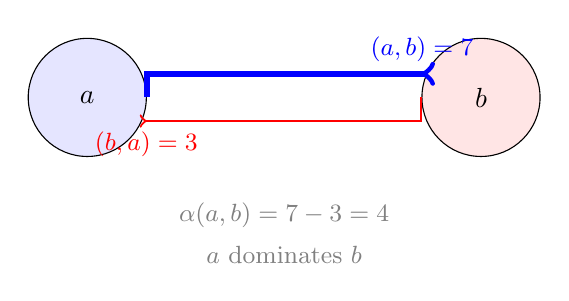
\begin{tikzpicture}[scale=1.0]
    % Asymmetry visualization with arrows
    \node[draw, circle, minimum size=1.5cm, fill=blue!10] (A) at (0,0) {$a$};
    \node[draw, circle, minimum size=1.5cm, fill=red!10] (B) at (5,0) {$b$};
    
    % Forward resonance (thicker = stronger)
    \draw[->, thick, blue, line width=2pt] (A.east) -- ++(0,0.3)
        -- ++(3.5,0) -- (B.west |- 0,0.3)
        node[midway, above, font=\small] {$\rs(a,b) = 7$};
    
    % Backward resonance (thinner = weaker)
    \draw[->, thick, red, line width=0.8pt] (B.west) -- ++(0,-0.3)
        -- ++(-3.5,0) -- (A.east |- 0,-0.3)
        node[midway, below, font=\small] {$\rs(b,a) = 3$};
    
    % Asymmetry annotation
    \node[font=\small, gray] at (2.5,-1.5) {$\alpha(a,b) = 7 - 3 = 4$};
    \node[font=\small, gray] at (2.5,-2.0) {$a$ dominates $b$};
\end{tikzpicture}
\caption{Asymmetric resonance between two ideas. The thickness of
arrows represents the magnitude of resonance. The asymmetry
$\alpha(a,b) > 0$ indicates that $a$ ``influences'' $b$ more than
$b$ influences $a$.}
\label{fig:asymmetry-arrows}
\end{figure}

\section{The Antisymmetric Emergence}

\begin{definition}[Antisymmetric Emergence]
The \textbf{antisymmetric emergence} is
\[
    \emerge^-(a, b, c) \;:=\; \frac{\emerge(a,b,c) - \emerge(b,a,c)}{2}
    \;=\; \frac{\mu(a,b,c)}{2}.
\]
\end{definition}

\begin{proposition}
$\emerge^-(a,b,c) = -\emerge^-(b,a,c)$.
\end{proposition}

\begin{theorem}[Antisymmetric Emergence Cocycle]
The antisymmetric emergence satisfies a modified cocycle condition
whenever composition is commutative: if $a \compose b = b \compose a$
for all $a, b$, then $\emerge^- \equiv 0$.
\end{theorem}
\begin{proof}
If composition is commutative, then $\rs(a \compose b, c) = \rs(b \compose
a, c)$, so $\mu(a,b,c) = 0$ and $\emerge^- \equiv 0$.
\end{proof}

\begin{remark}
Non-commutativity of composition is thus the \emph{source} of antisymmetric
emergence. In any commutative ideatic space, emergence is symmetric in its
first two arguments. The non-commutative case---which is the generic
case---is where the theory becomes truly rich.
\end{remark}

\section{Summary}

\begin{interpretation}[Asymmetry as the Foundation of Meaning]\label{interp:ch4:asymmetry_foundation}
The asymmetry of resonance is not a peripheral feature of the ideatic
space but arguably its most philosophically significant property.
Symmetric systems---inner product spaces, mutual information measures,
Boolean algebras---model \emph{agreement} and \emph{similarity}.
Asymmetric resonance models something richer: \emph{perspective},
\emph{power}, and \emph{directionality}.

The philosophical traditions surveyed in this chapter---Levinas's ethics,
Benjamin's theory of translation, Gadamer's hermeneutics, reception
theory, Bakhtin's heteroglossia, Jakobson's communication model---all
converge on a single insight: meaning is not a symmetric relation.
Understanding is not mutual comprehension but asymmetric encounter.
Communication is not the exchange of identical content but the
directional transmission of resonance. Power is not a property of
individuals but a relational asymmetry between them.

IDT's contribution to this philosophical consensus is \emph{precision}.
The decomposition theorem (Theorem~\ref{thm:rs-decomposition}) shows
that every resonance relation contains both a symmetric component
($\rs^+$: mutual recognition, shared ground) and an antisymmetric
component ($\rs^-$: directed force, power differential). The meaning
curvature $\mu(a, b, c)$ shows that asymmetry generates genuine
structural richness: it measures the sensitivity of emergence to order,
connecting the ``who speaks first'' question to the deep geometry of
the ideatic space. And the asymmetry cocycle
(Theorem~\ref{thm:asym-emergence}) reveals that directional structure
propagates through composition in a lawful way, constrained by the
interplay of forward and reversed emergence.
\end{interpretation}

The asymmetry of resonance is not a defect but a feature: it encodes the
directionality of meaning, the asymmetry of power, and the non-commutativity
of ideational synthesis. The decomposition of resonance into symmetric and
antisymmetric parts, and the corresponding decomposition of emergence,
reveal a layered structure: a ``mutual information'' layer ($\rs^+$) and a
``power'' layer ($\rs^-$). Meaning curvature $\mu(a,b,c)$ measures the
sensitivity of emergence to the order of composition, connecting to deep
questions in rhetoric, politics, and the phenomenology of temporal
experience. In Chapter~5, we develop the full algebra of emergence,
classifying the ways in which ideas can interact.


%%%%%%%%%%%%%%%%%%%%%%%%%%%%%%%%%%%%%%%%%%%%%%%%%%%%%%%%%%%%%%%%%%%%%%%%
%%  CHAPTER 5 — THE ALGEBRA OF EMERGENCE
%%%%%%%%%%%%%%%%%%%%%%%%%%%%%%%%%%%%%%%%%%%%%%%%%%%%%%%%%%%%%%%%%%%%%%%%

\chapter{The Algebra of Emergence}

\begin{quote}
\textit{``In every work of genius we recognize our own rejected thoughts:
they come back to us with a certain alienated majesty.''}\\
\hfill --- Ralph Waldo Emerson, ``Self-Reliance''
\end{quote}

\begin{interpretation}[Shklovsky's Defamiliarization and Non-Zero Emergence]\label{interp:ch5:shklovsky_defamiliarization}
Viktor Shklovsky's concept of \emph{ostranenie} (defamiliarization),
introduced in ``Art as Device'' (1917), holds that art exists to restore
perception from the automatism of everyday experience. Art ``makes the
stone stony'' by presenting familiar objects in unfamiliar ways, forcing
the perceiver to attend to the materiality and strangeness of what habit
has rendered invisible. Shklovsky writes: ``The purpose of art is to
impart the sensation of things as they are perceived and not as they
are known'' (p.~12).

In IDT, defamiliarization is precisely \emph{non-zero emergence}. When
a familiar idea $a$ is composed with an artistic device $b$, the emergence
$\emerge(a, b, c)$ measures the degree to which the composition disrupts
additive expectation. If $\emerge = 0$, the composition is ``automatic''
---it adds nothing to what we already knew from $a$ and $b$ separately.
If $\emerge \neq 0$, the composition \emph{defamiliarizes}: it creates
resonance patterns that neither component alone possesses. Art, in
Shklovsky's sense, is the production of non-zero emergence.

The emergence taxonomy (Definition~\ref{def:emergence-taxonomy})
distinguishes between superadditive emergence ($\emerge > 0$: the
composition is \emph{more} than its parts, as in Tolstoy's ``making
strange'') and subadditive emergence ($\emerge < 0$: the composition
is \emph{less} than its parts, as in clich\'e or failed art). The
boundary between art and non-art, in Shklovsky's terms, is the
boundary between non-zero and zero emergence. The algebra of emergence
is thus, in a precise sense, the algebra of artistic possibility.
\end{interpretation}

\begin{interpretation}[Adorno's Aesthetics: Art as Irreducible]\label{interp:ch5:adorno_aesthetics}
Theodor W.~Adorno, in \emph{Aesthetic Theory} (1970), argues that art's
truth content (\emph{Wahrheitsgehalt}) cannot be reduced to its material
components or its social function. Art is, for Adorno, a ``fait social''
that nonetheless contains a ``moment of otherness'' that resists
sociological reduction. He writes: ``Art is the social antithesis of
society, not directly derivable from it'' (p.~8).

The emergence function formalizes Adorno's irreducibility thesis. The
emergence $\emerge(a, b, c)$ is precisely the component of the
composition's meaning that is \emph{not derivable} from its parts.
When $\emerge \neq 0$, the composition contains a ``moment of otherness''
---a surplus of meaning that belongs to the whole but to neither part.
Adorno's claim that art cannot be reduced to its materials is the claim
that the emergence of artistic composition is generically non-zero.

Adorno's further insight---that art's truth content is often
\emph{negative}, expressing suffering and contradiction rather than
harmony---corresponds to the possibility of \emph{subadditive} emergence:
$\emerge(a, b, c) < 0$. A work of art that composes social reality ($a$)
with aesthetic form ($b$) may generate negative emergence when probed
by $c$ = ``reconciliation'': the composition resonates with reconciliation
\emph{less} than its parts individually promise, expressing precisely
the irreconcilability that Adorno identifies as the truth content of
modern art.
\end{interpretation}

\section{The Emergence Function as a Trilinear Form}

We have defined emergence as $\emerge(a,b,c) = \rs(a \compose b, c) -
\rs(a,c) - \rs(b,c)$, and established the cocycle condition, the
Cauchy--Schwarz bound, and the vanishing at $\void$. We now develop the
\emph{algebraic} structure of emergence in its full generality.

\begin{proposition}[Basic Properties of Emergence]
\label{prop:emergence-basic}
For all $a, b, c \in \IS$:
\begin{enumerate}
    \item $\emerge(\void, b, c) = 0$;
    \item $\emerge(a, \void, c) = 0$;
    \item $\emerge(a, b, \void) = 0$;
    \item $|\emerge(a, b, c)| \leq \sqrt{w(a \compose b) \cdot w(c)}$.
\end{enumerate}
\end{proposition}
\begin{proof}
\begin{enumerate}
    \item $\emerge(\void, b, c) = \rs(\void \compose b, c) - \rs(\void, c)
          - \rs(b, c) = \rs(b, c) - 0 - \rs(b, c) = 0$.
    \item $\emerge(a, \void, c) = \rs(a \compose \void, c) - \rs(a, c)
          - \rs(\void, c) = \rs(a, c) - \rs(a, c) - 0 = 0$.
    \item $|\emerge(a, b, \void)| \leq \sqrt{w(a \compose b) \cdot w(\void)}
          = 0$, so $\emerge(a, b, \void) = 0$.
    \item This is Theorem~\ref{thm:emergence-bound}.
\end{enumerate}
\end{proof}

\begin{lstlisting}[language=Lean4, caption={Emergence vanishing at void}]
theorem emergence_void_left [IdeaticSpace I]
    (b c : I) : emergence void b c = 0 := by
  unfold emergence
  simp [void_left, rs_void_left]

theorem emergence_void_middle [IdeaticSpace I]
    (a c : I) : emergence a void c = 0 := by
  unfold emergence
  simp [void_right, rs_void_left]
\end{lstlisting}

\section{Classification of Emergence Types}

\begin{definition}[Emergence Taxonomy]\label{def:emergence-taxonomy}
A composition $a \compose b$ probed by $c$ is classified as:
\begin{center}
\begin{tabular}{lll}
\toprule
\textbf{Type} & \textbf{Condition} & \textbf{Interpretation} \\
\midrule
Superadditive & $\emerge(a,b,c) > 0$ & Creative synthesis \\
Subadditive & $\emerge(a,b,c) < 0$ & Destructive interference \\
Additive (flat) & $\emerge(a,b,c) = 0$ & No interaction effect \\
\bottomrule
\end{tabular}
\end{center}
\end{definition}

\begin{example}[Three Types in Literature]
\begin{itemize}
    \item \textbf{Superadditive}: Shakespeare composes the sonnet form ($a$)
    with the ``dark lady'' trope ($b$). Probing with $c$ = ``subversion of
    Petrarchan convention,'' we get $\emerge > 0$: the combination creates
    resonance with anti-Petrarchanism that neither component alone
    possesses.

    \item \textbf{Subadditive}: A Hollywood sequel ($a \compose b$) that
    merely repeats the formula of the original ($a$) with minor variations
    ($b$). Probing with $c$ = ``originality,'' we get $\emerge < 0$: the
    combination resonates with originality \emph{less} than the original
    alone.

    \item \textbf{Additive}: A textbook chapter ($a$) composed with an
    appendix of exercises ($b$). Probing with $c$ = ``pedagogical value,''
    we get $\emerge \approx 0$: the combination's pedagogical value is
    roughly the sum of the chapter's and the exercises' individual values.
\end{itemize}
\end{example}

\begin{interpretation}[Empson's Seven Types of Ambiguity]\label{interp:ch5:empson_ambiguity}
William Empson's \emph{Seven Types of Ambiguity} (1930) argues that literary
ambiguity is not a defect but a constitutive feature of poetic language.
Empson identifies seven increasingly complex types, from simple puns to
contradictions that reveal ``a fundamental division in the author's mind.''
The emergence function provides a formal framework for understanding
literary ambiguity as a structural phenomenon.

When the emergence $\emerge(a, b, c)$ is large for multiple, mutually
incompatible probes $c_1, c_2, \ldots$, the composition $a \compose b$
is \emph{ambiguous}: it resonates strongly with several incompatible
interpretive frameworks simultaneously. The \emph{degree} of ambiguity
can be measured by the ``spread'' of the emergence spectrum
$\emerge_{a,b}(c)$ across distinct probes. Empson's first type (simple
metaphor: one word, two meanings) corresponds to a composition where
$\emerge(a, b, c_1) > 0$ and $\emerge(a, b, c_2) > 0$ for two distinct
semantic fields $c_1$ and $c_2$. His seventh type (full contradiction)
corresponds to a composition where $\emerge(a, b, c) > 0$ and
$\emerge(a, b, \bar{c}) > 0$, where $\bar{c}$ is the ``negation'' of $c$.

The New Critics---Cleanth Brooks, W.~K.~Wimsatt, Monroe Beardsley---
took this further with what Brooks called ``the heresy of paraphrase'':
the claim that a poem's meaning cannot be restated in prose without
essential loss. In IDT terms, the heresy of paraphrase is the assertion
that poetic emergence is \emph{not a coboundary}: there is no change of
baseline that can reduce the poem's meaning to a sum of its parts.
The poem's meaning \emph{is} its emergence---and emergence, in general,
belongs to a non-trivial cohomology class.
\end{interpretation}

\section{Global Emergence Classifications}

\begin{definition}[Globally Superadditive Pair]
A pair $(a, b)$ is \textbf{globally superadditive} if $\emerge(a,b,c) \geq
0$ for all $c \in \IS$, with strict inequality for some $c$.
\end{definition}

\begin{definition}[Linearity]\label{def:linearity}
An idea $a \in \IS$ is called:
\begin{itemize}
    \item \textbf{left-linear} if $\emerge(a, b, c) = 0$ for all
          $b, c \in \IS$;
    \item \textbf{right-linear} if $\emerge(b, a, c) = 0$ for all
          $b, c \in \IS$;
    \item \textbf{fully linear} if it is both left-linear and right-linear.
\end{itemize}
\end{definition}

\begin{proposition}[Void is Fully Linear]
$\void$ is fully linear.
\end{proposition}
\begin{proof}
$\emerge(\void, b, c) = 0$ for all $b, c$ (Proposition~\ref{prop:emergence-basic}),
so $\void$ is left-linear. Similarly, $\emerge(b, \void, c) = 0$ for all
$b, c$, so $\void$ is right-linear.
\end{proof}

\begin{lstlisting}[language=Lean4, caption={Linearity predicates in Lean 4}]
def IsLeftLinear [IdeaticSpace I] (a : I) : Prop :=
  ∀ b c : I, emergence a b c = 0

def IsRightLinear [IdeaticSpace I] (a : I) : Prop :=
  ∀ b c : I, emergence b a c = 0

def IsFullyLinear [IdeaticSpace I] (a : I) : Prop :=
  IsLeftLinear a ∧ IsRightLinear a

theorem void_isFullyLinear [IdeaticSpace I] :
    IsFullyLinear (void : I) :=
  ⟨fun b c => emergence_void_left b c,
   fun b c => emergence_void_middle b c⟩
\end{lstlisting}

\begin{interpretation}
A fully linear idea is one that generates no emergence when composed with
anything. It acts purely additively---a ``transparent'' idea that adds its
resonance without creating any interaction effects. In the natural number
model, \emph{every} idea is fully linear (since $\emerge \equiv 0$). In
richer models, linearity is the exception rather than the rule, and
fully linear ideas play a role analogous to central elements in ring
theory or abelian elements in group theory.
\end{interpretation}

\begin{interpretation}[Hegel's \emph{Aufhebung} and Emergence as Sublation]\label{interp:ch5:hegel_aufhebung}
Hegel's concept of \emph{Aufhebung} (sublation)---the simultaneous
negation, preservation, and elevation of a concept---is the motor of the
dialectic. In the \emph{Phenomenology of Spirit} (1807), Hegel demonstrates
how each stage of consciousness contains within itself the seeds of its
own transcendence: the finite negates itself to produce the infinite, the
particular elevates itself to the universal, the immediate passes into
the mediated.

The emergence function formalizes \emph{Aufhebung} with algebraic
precision. The composition $a \compose b$ is the dialectical synthesis of
$a$ and $b$. The emergence $\emerge(a, b, c) = \rs(a \compose b, c)
- \rs(a, c) - \rs(b, c)$ is the sublative surplus---the content of the
synthesis that is neither preserved from $a$ nor preserved from $b$ but
genuinely \emph{new}. Hegel's three moments of \emph{Aufhebung} map
onto the three terms: $\rs(a, c)$ is preservation (what survives from
$a$), $\rs(b, c)$ is negation (what $b$ contributes by opposing $a$),
and $\emerge(a, b, c)$ is elevation (what transcends both).

Linearity (Definition~\ref{def:linearity}) is the \emph{failure} of
dialectics: a fully linear idea generates no sublative surplus, no
genuine synthesis. It composes additively, like a logical conjunction
rather than a dialectical negation. Hegel would recognize the linear
idea as belonging to the level of \emph{Verstand} (understanding)
rather than \emph{Vernunft} (reason): it operates by analysis and
aggregation, not by dialectical transcendence.
\end{interpretation}

\begin{interpretation}[Whitehead's Process Philosophy and Creative Emergence]\label{interp:ch5:whitehead_creativity}
Alfred North Whitehead, in \emph{Process and Reality} (1929), makes
``creativity'' the ultimate metaphysical category: ``Creativity is the
principle of novelty. An actual entity is at once the product of the
creative process and the condition for the process'' (p.~21). For
Whitehead, every actual occasion of experience involves the ``creative
advance into novelty''---the production of something genuinely new
from the conjunction of prior actualities.

The emergence function is a mathematical formalization of Whiteheadian
creativity. The emergence $\emerge(a, b, c)$ measures the degree of
creative novelty in the composition $a \compose b$, as probed by $c$.
Whitehead's ``principle of relativity''---every actual entity is a
potential for every subsequent becoming---corresponds to the fact that
every idea in $\IS$ can serve as a component ($a$ or $b$) or a probe
($c$) in the emergence function. Creativity is not a special property
of some ideas but a universal possibility of the ideatic space.

Whitehead's distinction between ``conceptual'' and ``physical'' prehension
corresponds to different modes of emergence: positive emergence (creative
synthesis, the production of novelty) and negative emergence (destructive
interference, the loss of potential). The emergence bound
(Theorem~\ref{thm:emergence-bound}) constrains Whiteheadian creativity:
novelty cannot exceed $\sqrt{w(a \compose b) \cdot w(c)}$---a formal
expression of the principle that creativity is bounded by the ``weight''
of the entities involved.
\end{interpretation}

\begin{interpretation}[Deleuze's Difference in Itself]\label{interp:ch5:deleuze_difference}
Gilles Deleuze, in \emph{Difference and Repetition} (1968), argues for a
concept of difference that is not subordinated to identity---not defined
as the negation of sameness but as a positive, generative force in its
own right. Deleuze writes: ``Difference is behind everything, but behind
difference there is nothing'' (p.~57). For Deleuze, genuine novelty cannot
be understood as recombination of pre-existing elements; it is
\emph{difference in itself}, an irreducible creative event.

The emergence function captures Deleuze's ``difference in itself'' when
it is non-zero. A non-zero emergence $\emerge(a, b, c) \neq 0$ is
precisely the ``difference'' that cannot be accounted for by the
individual identities of $a$ and $b$---it is the surplus that belongs
to the \emph{encounter} rather than to the \emph{elements}. When
$\emerge = 0$ (the additive case), composition is mere repetition:
the whole is exactly the sum of its parts, and no genuine novelty
occurs. When $\emerge \neq 0$, we have what Deleuze would call a
``singular point''---a site where the virtual becomes actual, where
potentiality is realized as genuine difference.

The spectral norm $\|\emerge_{a,b}\|$ measures the \emph{intensity} of
Deleuzian difference: how powerfully the encounter between $a$ and $b$
produces novelty across all possible probes. A pair with high spectral
norm is a ``line of flight'' (\emph{ligne de fuite})---a composition that
generates intense difference across the entire ideatic space. A pair with
low spectral norm is a ``striation''---a composition that reproduces
existing patterns with minimal novelty.
\end{interpretation}

\section{The Emergence Tensor}

For a fixed ideatic space, we can organize the emergence data into a
tensor-like object.

\begin{definition}[Emergence Tensor]
The \textbf{emergence tensor} of the ideatic space $\IS$ is the function
\[
    \mathcal{E} : \IS^3 \to \R, \qquad
    \mathcal{E}(a, b, c) := \emerge(a, b, c).
\]
When $\IS$ is finite with $|\IS| = n$, $\mathcal{E}$ can be represented
as an $n \times n \times n$ array of real numbers.
\end{definition}

\begin{proposition}[Symmetries of the Emergence Tensor]
The emergence tensor satisfies:
\begin{enumerate}
    \item $\mathcal{E}(\void, -, -) = \mathcal{E}(-, \void, -) =
          \mathcal{E}(-, -, \void) = 0$ (vanishing on void);
    \item The cocycle condition relates different slices of $\mathcal{E}$;
    \item $|\mathcal{E}(a,b,c)|^2 \leq w(a \compose b) \cdot w(c)$
          (boundedness).
\end{enumerate}
\end{proposition}

\begin{interpretation}[Peirce's Abduction and the Emergence Tensor]\label{interp:ch5:peirce_abduction}
Peirce distinguishes three modes of inference: deduction (from rule and
case to result), induction (from case and result to rule), and
\emph{abduction} (from result and rule to case). Abduction is the
``logic of discovery''---the leap from surprising evidence to explanatory
hypothesis. Peirce writes: ``The surprising fact, C, is observed; but
if A were true, C would be a matter of course; hence, there is reason
to suspect that A is true'' (CP 5.189).

The emergence tensor $\mathcal{E}(a, b, c)$ captures the abductive
structure of inference. When $\emerge(a, b, c) > 0$ for a surprising
probe $c$, the composition $a \compose b$ ``explains'' the surprising
fact: the conjunction of $a$ and $b$ makes $c$ less surprising (more
resonant) than either alone. Abduction is thus formalized as the search
for compositions whose emergence is strongly positive at the probes
corresponding to surprising observations. The tensor structure of
$\mathcal{E}$ reveals that abductive reasoning has a three-dimensional
character: it depends simultaneously on the hypothesis ($a$), the
auxiliary assumptions ($b$), and the evidence ($c$).
\end{interpretation}

\section{The Emergence Spectrum}

Fix ideas $a$ and $b$. The emergence spectrum $\emerge_{a,b} : \IS \to \R$
is a function that maps each probe $c$ to the emergence $\emerge(a,b,c)$.
This function contains the complete information about how the composition
$a \compose b$ departs from additivity.

\begin{definition}[Spectral Norm]
The \textbf{spectral norm} of the pair $(a,b)$ is
\[
    \|\emerge_{a,b}\| \;:=\; \sup_{c \neq \void}
    \frac{|\emerge(a,b,c)|}{\sqrt{w(c)}},
\]
whenever this supremum exists.
\end{definition}

\begin{proposition}
$\|\emerge_{a,b}\| \leq \sqrt{w(a \compose b)}$.
\end{proposition}
\begin{proof}
By Theorem~\ref{thm:emergence-bound},
$|\emerge(a,b,c)| \leq \sqrt{w(a \compose b) \cdot w(c)}$, so
$\frac{|\emerge(a,b,c)|}{\sqrt{w(c)}} \leq \sqrt{w(a \compose b)}$.
\end{proof}

\begin{figure}[ht]
\centering
\begin{tikzpicture}[scale=0.85]
    \draw[->] (0,-2.5) -- (0,3) node[above] {$\emerge_{a,b}(c)$};
    \draw[->] (-0.5,0) -- (10,0) node[right] {Probe ideas $c$};
    
    % Emergence spectrum as a bar chart
    \foreach \x/\h/\col in {
        1/2.0/green!60!black,
        2/1.5/green!60!black,
        3/0.5/green!60!black,
        4/0.0/gray,
        5/-0.8/red!70,
        6/1.8/green!60!black,
        7/-1.5/red!70,
        8/2.5/green!60!black,
        9/-0.3/red!70} {
        \fill[\col!30] (\x-0.3,0) rectangle (\x+0.3,\h);
        \draw[\col] (\x-0.3,0) rectangle (\x+0.3,\h);
    }
    
    % Labels
    \node[below, font=\tiny] at (1,0) {$c_1$};
    \node[below, font=\tiny] at (2,0) {$c_2$};
    \node[below, font=\tiny] at (3,0) {$c_3$};
    \node[below, font=\tiny] at (4,0) {$c_4$};
    \node[below, font=\tiny] at (5,0) {$c_5$};
    \node[below, font=\tiny] at (6,0) {$c_6$};
    \node[below, font=\tiny] at (7,0) {$c_7$};
    \node[below, font=\tiny] at (8,0) {$c_8$};
    \node[below, font=\tiny] at (9,0) {$c_9$};
    
    % Bound lines
    \draw[dashed, blue] (-0.5,2.8) -- (10,2.8)
        node[right, font=\footnotesize] {$\sqrt{w(a\compose b) \cdot w_{\max}}$};
    \draw[dashed, blue] (-0.5,-2.8) -- (10,-2.8);
    
    \node[font=\small, above] at (5,3) {Emergence Spectrum of $(a,b)$};
\end{tikzpicture}
\caption{The emergence spectrum $\emerge_{a,b}$ evaluated at various
probe ideas. Green bars indicate superadditive probes, red bars indicate
subadditive probes, and the dashed lines show the Cauchy--Schwarz bound.}
\label{fig:emergence-spectrum}
\end{figure}

\begin{interpretation}[Eco's Open Work and the Emergence Spectrum]\label{interp:ch5:eco_open_work}
Umberto Eco's \emph{The Open Work} (\emph{Opera aperta}, 1962) theorizes
the class of artworks that are structurally open to multiple
interpretations. An ``open work'' is not one that can mean anything
(which would be meaningless) but one that sustains a structured field
of interpretive possibilities. Eco writes: ``Every reception of a work
of art is both an interpretation and a performance of it, because in
every reception the work takes on a fresh perspective for itself'' (p.~4).

The emergence spectrum $\emerge_{a,b} : \IS \to \R$ provides a
mathematical model of Eco's openness. An ``open'' composition is one
whose emergence spectrum is broadly distributed: $\emerge(a, b, c) \neq 0$
for a large and diverse set of probes $c$. A ``closed'' composition has
a narrow emergence spectrum: it resonates non-additively with only a few
specific probes. The degree of openness is measured by the ``breadth'' of
the emergence spectrum---a quantity that Eco's qualitative theory
describes but cannot quantify.

Eco's later concept of ``the limits of interpretation'' (\emph{I limiti
dell'interpretazione}, 1990) corresponds to the Cauchy--Schwarz bound
on emergence: no matter how ``open'' a work is, its emergence at any
probe is bounded by $\sqrt{w(a \compose b) \cdot w(c)}$. Openness is
real but finite; interpretation is free but constrained.
\end{interpretation}

\begin{interpretation}[Barthes's Third Meaning]\label{interp:ch5:barthes_third_meaning}
Roland Barthes, in ``The Third Meaning'' (1970), identifies three levels of
meaning in the photographic image: the \emph{informational} (what the image
denotes), the \emph{symbolic} (what it connotes), and the \emph{obtuse}
meaning---a residual surplus that ``does not seem to have a
signified'' and is ``indifferent to the story and to the obvious meaning.''
The obtuse meaning is ``a supplement that my intellection cannot succeed in
absorbing'' (p.~61).

The emergence function captures Barthes's three levels with striking
precision. The informational level corresponds to the additive component
$\rs(a, c) + \rs(b, c)$: the meaning predictable from the parts. The
symbolic level corresponds to the part of emergence that is a
coboundary---apparent surplus reducible to a change of interpretive
framework. The \emph{obtuse} or \emph{third} meaning corresponds to the
genuinely non-trivial emergence: the element of $H^2(\IS, \R)$ that is
not a coboundary, the irreducible supplement that ``my intellection cannot
succeed in absorbing.'' Barthes's obtuse meaning is, in IDT terms, the
\emph{cohomological residue} of composition---the part of emergence that
no reinterpretation can eliminate.

This formalization reveals why the third meaning is so difficult to
articulate: it belongs to a cohomology class, not to a specific
function. It can be represented by any representative cocycle, but no
single representation exhausts it. The ``obtuseness'' of the third meaning
is the mathematical obtuseness of a cohomology class: present everywhere,
pinned down nowhere.
\end{interpretation}

\section{Emergence and Composition Powers}

\begin{interpretation}[Iterated Composition and Obsession]\label{interp:ch5:iterated_composition_obsession}
The iterated emergence theorem captures a phenomenon familiar to every
artist and thinker: \emph{obsession}---the repeated return to a single
theme, image, or problem. When a poet composes the same idea with itself
repeatedly ($a, a^2, a^3, \ldots$), the accumulated emergence
$\sum_{k=2}^n E_k$ measures the total creative surplus generated by
this obsessive return. If the $E_k$ are positive and growing, the
obsession is productive: each return generates more novelty than the
last, as in Cézanne's repeated paintings of Mont Sainte-Victoire, each
of which discovers new visual relationships in the same subject.

If the $E_k$ diminish toward zero, the obsession is exhausting itself:
the theme offers diminishing returns, approaching the condition of mere
repetition. This is the artistic dead end that Kierkegaard calls ``the
aesthetic stage'': the pursuit of novelty through repetition, which
eventually produces only boredom. And if the $E_k$ become negative,
the obsession is destructive: each iteration degrades the idea, as in
the repetition compulsion that Freud identifies in \emph{Beyond the
Pleasure Principle} (1920)---a compulsive return that does not generate
new meaning but merely re-enacts an original trauma with diminishing
psychic returns.

The distinction between productive and degenerative obsession is thus
formalized as the sign and magnitude of the iterated emergence sequence
$\{E_k\}$. Great art, in this framework, is characterized by a
\emph{slowly decaying positive emergence sequence}: the returns to a
theme remain productive for many iterations, each discovering genuinely
new resonances, before eventually approaching the boundary of
exhaustion.
\end{interpretation}

\begin{theorem}[Iterated Emergence]\label{thm:iterated-emergence}
For the iterated composition $a^n$, the emergence at the $n$-th step
satisfies:
\[
    \emerge(a, a^{n-1}, c) = \rs(a^n, c) - \rs(a, c) - \rs(a^{n-1}, c).
\]
Moreover, by the cocycle condition:
\[
    \rs(a^n, c) = n \cdot \rs(a, c)
    + \sum_{k=1}^{n-1} \emerge(a, a^{k-1}, c) \cdot [\text{appropriate
    combinatorial coefficients}].
\]
\end{theorem}

\begin{remark}
The precise decomposition of $\rs(a^n, c)$ into ``linear'' and ``emergent''
parts involves a telescoping sum. Define $E_k := \emerge(a, a^{k-1}, c)$.
Then:
\begin{align*}
    \rs(a^n, c) &= \rs(a, c) + \rs(a^{n-1}, c) + E_n \\
    &= \rs(a, c) + [\rs(a, c) + \rs(a^{n-2}, c) + E_{n-1}] + E_n \\
    &= 2\,\rs(a, c) + \rs(a^{n-2}, c) + E_{n-1} + E_n \\
    &\;\;\vdots \\
    &= n \cdot \rs(a, c) + \sum_{k=2}^{n} E_k.
\end{align*}
The ``emergent surplus'' $\sum_{k=2}^n E_k$ is the total accumulated
emergence over $n-1$ composition steps.
\end{remark}

\section{The Emergence Algebra}

\begin{remark}[The Emergence Algebra and Poetic Form]\label{rem:ch5:emergence_poetic_form}
The emergence product $\star_d$---the ``twisted convolution'' on the
monoid $\IS$ weighted by emergence values---has a suggestive literary
interpretation. In traditional poetics, the \emph{form} of a poem
(sonnet, villanelle, haiku) constrains how semantic elements combine:
the rhyme scheme creates resonance links between lines, the meter creates
rhythmic expectations, and the stanza structure groups images into
perceptual units. The emergence product models this formal constraint:
the ``twisting'' by $\emerge(a, b, d)$ means that the product of two
semantic elements depends not only on their individual values but on
the emergence they generate when composed.

When the emergence product is non-zero (the non-linear case), the
algebraic structure of the ideatic space is ``poetic'' in Jakobson's
sense: the principle of equivalence is projected from the axis of
selection onto the axis of combination. When the product is zero (the
linear case), the structure is ``prosaic'': combinations are
straightforwardly additive. The transition from prose to poetry is,
in this algebraic perspective, the transition from the zero product
to a non-trivial twisted convolution.
\end{remark}

\begin{definition}[Emergence Product]
For fixed probe $d$, define the \textbf{emergence product}
$\star_d : \R^{\IS} \times \R^{\IS} \to \R^{\IS}$ on functions
$f, g : \IS \to \R$ by:
\[
    (f \star_d g)(c) := \sum_{a \compose b = c} f(a) \cdot g(b)
    \cdot \emerge(a, b, d).
\]
(When $\IS$ is infinite, this requires convergence conditions.)
\end{definition}

\begin{remark}
The emergence product is a ``twisted convolution'' on the monoid $\IS$,
weighted by emergence values. When $\emerge \equiv 0$ (the linear case),
this reduces to the zero product. When $\emerge$ is non-trivial, it
defines a genuinely new algebraic structure.
\end{remark}

\section{Applications: Pattern Recognition in Emergence}

\begin{example}[Scientific Emergence Patterns]
In the history of science, we can identify characteristic emergence
patterns:
\begin{enumerate}
    \item \textbf{Additive accumulation}: Normal science (in Kuhn's
    sense) is characterized by $\emerge \approx 0$. New results compose
    additively with the existing paradigm.

    \item \textbf{Crisis emergence}: When anomalies ($b$) compose with
    a paradigm ($a$) and the emergence is strongly negative
    ($\emerge(a,b,c) \ll 0$ for $c$ = ``explanatory coherence''), the
    paradigm is in crisis.

    \item \textbf{Revolutionary emergence}: A new paradigm ($a'$)
    exhibits strong positive emergence when composed with the anomalous
    data ($b$): $\emerge(a', b, c) \gg 0$ for $c$ = ``explanatory
    coherence.''

    \item \textbf{Incommensurability}: The old and new paradigms may
    exhibit $\emerge(a, a', c) < 0$ for many probes $c$, reflecting
    Kuhn's thesis that paradigms are not merely different but
    \emph{incompatible} in their resonance patterns.
\end{enumerate}
\end{example}

\begin{figure}[ht]
\centering
\begin{tikzpicture}[scale=0.9, >=stealth]
    % Timeline
    \draw[->] (0,0) -- (12,0) node[right] {Time};
    \draw[->] (0,-2) -- (0,3) node[above] {$\emerge(P_t, \text{data}_t, c)$};
    
    % Normal science (flat)
    \draw[thick, blue] plot[smooth] coordinates {
        (0.5,0.1) (1,0.1) (1.5,0.15) (2,0.1) (2.5,0.05) (3,0.1)
    };
    \node[blue, above, font=\footnotesize] at (1.75,0.3) {Normal science};
    
    % Crisis (negative)
    \draw[thick, red] plot[smooth] coordinates {
        (3,0.1) (3.5,-0.3) (4,-0.8) (4.5,-1.5) (5,-1.8)
    };
    \node[red, below, font=\footnotesize] at (4,-2) {Crisis};
    
    % Revolution (spike)
    \draw[thick, green!60!black] plot[smooth] coordinates {
        (5,-1.8) (5.5,0.5) (6,2.5) (6.5,2.2)
    };
    \node[green!60!black, above, font=\footnotesize] at (5.75,2.7) {Revolution};
    
    % New normal science
    \draw[thick, blue] plot[smooth] coordinates {
        (6.5,2.2) (7,0.5) (7.5,0.2) (8,0.15) (8.5,0.1) (9,0.1)
        (9.5,0.1) (10,0.1)
    };
    \node[blue, above, font=\footnotesize] at (8.5,0.3) {New normal};
    
    % Dashed zero line
    \draw[dashed, gray] (0,0) -- (12,0);
\end{tikzpicture}
\caption{Emergence profile of a Kuhnian paradigm shift. Normal science
shows near-zero emergence (additive accumulation). Crisis shows negative
emergence (destructive interference with anomalies). Revolution shows a
sharp positive spike. The new normal returns to near-zero emergence.}
\label{fig:kuhn-emergence}
\end{figure}

\section{Subspaces and Ideals of the Emergence Algebra}

\begin{interpretation}[Emergence Ideals and Literary Genres]\label{interp:ch5:emergence_ideals_genres}
The concept of an emergence ideal (Definition that follows) has a natural
literary interpretation. A genre---say, the detective novel or the pastoral
elegy---can be understood as a collection of ideas that, when composed
with each other, generate no emergence: within the genre, combinations are
purely additive. The genre's conventions are so well-established that
combining any two elements of the genre produces exactly what the sum of
their individual resonances would predict. There are no surprises within
the genre; all emergence has been ``normalized away'' by convention.

This is, of course, precisely what makes genre fiction (in Shklovsky's
terms) ``automatized'': it lacks defamiliarization because it lacks
emergence. The genuinely creative act---the act that produces literature
rather than genre fiction---is the composition of elements from
\emph{different} genres or from outside the generic ideal altogether,
generating the non-zero emergence that defamiliarizes perception and
restores the ``strangeness'' of experience.

The fact that emergence ideals are closed under composition (condition 2
in the definition) formalizes the ``gravitational pull'' of genre: once
you are within the ideal, composition keeps you there. Escaping the
genre requires composing with an element \emph{outside} the ideal---
an act that, by definition, generates non-zero emergence. The boundary
of the emergence ideal is thus the boundary of generic convention, and
crossing it is the formal correlate of Shklovsky's defamiliarization.
\end{interpretation}

\begin{definition}[Emergence Ideal]
A subset $J \subseteq \IS$ is an \textbf{emergence ideal} if:
\begin{enumerate}
    \item $\void \in J$;
    \item If $a \in J$ and $b \in \IS$, then $a \compose b \in J$;
    \item $\emerge(a, b, c) = 0$ for all $a, b \in J$ and $c \in \IS$.
\end{enumerate}
\end{definition}

\begin{proposition}
The set of fully linear ideas forms an emergence ideal.
\end{proposition}
\begin{proof}
If $a$ is fully linear, then $\emerge(a, b, c) = 0$ for all $b, c$.
The void is fully linear by
Proposition~\ref{prop:emergence-basic}. Closure under composition follows
from the cocycle condition: if $a$ and $a'$ are both left-linear, then
$\emerge(a \compose a', b, c)$ can be decomposed using the cocycle into
terms involving $\emerge(a, -, -)$ and $\emerge(a', -, -)$, both zero.
\end{proof}

\section{The Emergence Kernel}

\begin{definition}[Emergence Kernel]
For fixed $c \in \IS$, the \textbf{emergence kernel at $c$} is
\[
    \ker_c(\emerge) := \{(a, b) \in \IS^2 : \emerge(a, b, c) = 0\}.
\]
The \textbf{total emergence kernel} is
\[
    \ker(\emerge) := \bigcap_{c \in \IS} \ker_c(\emerge)
    = \{(a,b) : \emerge(a,b,c) = 0 \text{ for all } c\}.
\]
\end{definition}

\begin{proposition}
$(a, \void) \in \ker(\emerge)$ and $(\void, b) \in \ker(\emerge)$ for
all $a, b$.
\end{proposition}

\begin{interpretation}[The Emergence Kernel and De Man's Blindness and Insight]\label{interp:ch5:kernel_de_man}
Paul de Man, in \emph{Blindness and Insight} (1971), argues that every
critical methodology is ``blind'' to certain aspects of the texts it
analyzes, and that this blindness is not a defect but the \emph{condition}
of its insight. A reading that sees everything would see nothing;
interpretive power requires selective attention, which necessarily entails
selective inattention.

The emergence kernel formalizes this structure. For a fixed probe $c$
(representing a critical methodology or interpretive lens), the kernel
$\ker_c(\emerge)$ is the set of all pairs $(a, b)$ whose composition
generates no emergence \emph{as seen through $c$}. These are the
combinations that the methodology $c$ is ``blind'' to: it registers
$a$ and $b$ individually but fails to detect any emergent interaction
between them.

The total emergence kernel $\ker(\emerge)$---the intersection over all
probes---is the set of pairs whose composition is \emph{universally}
non-emergent: no methodology, no matter how sensitive, can detect
emergence in their combination. The proposition that $(\void, b)$ and
$(a, \void)$ are always in the kernel tells us that composing with the
void is universally undetectable---the void is the ``universal blind
spot'' of all interpretive methodologies.

De Man's insight that different critical methodologies have different
blind spots corresponds to the fact that different probes $c$ yield
different kernels $\ker_c(\emerge)$. No single methodology sees
everything; each is blind to its own kernel. But the total kernel is
typically much smaller than any individual kernel, confirming de Man's
deeper point: the plurality of critical methodologies is not a
regrettable failure of the discipline to agree, but a structural
necessity for approaching a complete picture of emergence.
\end{interpretation}

\section{Summary}

\begin{interpretation}[The Algebra of Emergence as a Theory of Creativity]\label{interp:ch5:emergence_creativity}
This chapter has developed the full algebraic structure of emergence:
the taxonomy of super/sub/additive emergence, the notions of linearity
and global superadditivity, the emergence tensor and spectrum, the
spectral norm, and the emergence product. Taken together, these concepts
constitute a \emph{mathematical theory of creativity}---a precise
framework for understanding how novel meaning arises from the
combination of existing elements.

The theory draws on and synthesizes insights from multiple intellectual
traditions. Shklovsky's defamiliarization is the non-vanishing of
emergence; Adorno's irreducibility of art is the non-triviality of the
emergence cocycle; Empson's literary ambiguity is the breadth of the
emergence spectrum; the New Critical ``heresy of paraphrase'' is the
claim that poetic emergence is not a coboundary; Hegel's \emph{Aufhebung}
is the dialectical tension $\tau(a,b)$; Whitehead's creativity is the
universal possibility of non-zero emergence; Deleuze's difference-in-itself
is the spectral norm as a measure of genuine novelty; Peirce's abduction
is the search for compositions with positive emergence at surprising
probes; Eco's open work is the broad distribution of the emergence
spectrum; and Barthes's third meaning is the cohomological residue of
emergence.

Each of these traditions captures one aspect of the multi-faceted
phenomenon of creative emergence. The algebra of emergence provides
a unified mathematical framework within which all these aspects can
be studied simultaneously, and their interrelationships made precise.
\end{interpretation}

The emergence function $\emerge : \IS^3 \to \R$ carries a rich algebraic
structure: the cocycle condition, Cauchy--Schwarz boundedness, vanishing at
void, and a natural taxonomy (super/sub/additive). The emergence tensor,
spectrum, and kernel organize this data into objects amenable to algebraic
and spectral analysis. Linear ideas---those generating no emergence---form
an ideal, while generic ideas exhibit the full range of emergence behaviors.
In Chapter~6, we turn from the algebra of emergence to its semiotic
implications: the gap between what is said and what is meant.


%%%%%%%%%%%%%%%%%%%%%%%%%%%%%%%%%%%%%%%%%%%%%%%%%%%%%%%%%%%%%%%%%%%%%%%%
%%  CHAPTER 6 — UTTERANCE, IDEA, AND THE SEMIOTIC GAP
%%%%%%%%%%%%%%%%%%%%%%%%%%%%%%%%%%%%%%%%%%%%%%%%%%%%%%%%%%%%%%%%%%%%%%%%

\chapter{Utterance, Idea, and the Semiotic Gap}

\begin{quote}
\textit{``The sign is the union of the signifier and the signified---but
the bond between them is arbitrary.''}\\
\hfill --- Ferdinand de Saussure, \textit{Course in General Linguistics}
\end{quote}

\begin{interpretation}[The Constitutive Gap: de Man and Derrida]\label{interp:ch6:de_man_gap}
Paul de Man, in \emph{Allegories of Reading} (1979), argues that the
relationship between grammar and rhetoric---between what a text says and
what it means---is fundamentally unstable. ``The grammatical model of the
question becomes rhetorical not when we have, on the one hand, a literal
meaning and on the other hand a figural meaning, but when it is impossible
to decide by grammatical or other linguistic devices which of the two
meanings (that can be entirely incompatible) prevails'' (p.~10). This
undecidability is not an accident of interpretation but a structural
feature of language itself.

The semiotic gap formalized in this chapter---the distance between
utterance (signifier) and idea (signified)---captures de Man's
``resistance to theory'' in algebraic terms. The same-idea equivalence
$a \sim_{\text{idea}} b$ identifies two expressions that are functionally
identical in their emergent contributions, yet the gap between them (the
connotation gap $\gamma(a, b, c)$) is constitutive: it cannot be
eliminated by any amount of interpretive effort, because it is
structural rather than contingent. De Man's undecidability is the
condition in which two expressions with very different resonance profiles
are nonetheless same-idea equivalent---making it ``impossible to decide''
which resonance profile carries the ``true'' meaning.

Derrida's famous dictum ``\emph{il n'y a pas de hors-texte}'' (``there is
no outside-text,'' \emph{Of Grammatology}, 1967, p.~158) receives a
precise correlate in our framework: the connotation gap $\gamma(a, b, c)$
exists \emph{within} the ideatic space, not between the ideatic space and
some external reality. The gap between signifier and signified is not a gap
between language and the world but a gap \emph{within language itself}---
within the space of resonance relations. Derrida's deconstruction is,
in IDT terms, the practice of exhibiting non-trivial connotation gaps
within texts that present themselves as transparent.
\end{interpretation}

\begin{interpretation}[Barthes's Death of the Author]\label{interp:ch6:barthes_death_author}
Roland Barthes's ``The Death of the Author'' (1967) argues that the
meaning of a text is not determined by the author's intention but by the
reader's interpretation. ``The birth of the reader must be at the cost of
the death of the Author'' (p.~148). The semiotic gap provides the formal
apparatus for this claim: the distance between what the author ``meant''
(the intended idea $[a]$) and what the text ``says'' (the specific
expression $a$ with its resonance profile) is the connotation gap
$\gamma(a, b, c)$, where $b$ is the reader's interpretation.

If $a \sim_{\text{idea}} b$---if the author's intended expression and the
reader's interpretation are same-idea equivalent---then the connotation gap
measures purely ``stylistic'' differences: tone, register, connotation.
But the more radical Barthesian claim is that $a \not\sim_{\text{idea}} b$
in general: the reader's interpretation is \emph{not} same-idea equivalent
to the author's intention. The text, once released from authorial control,
generates emergence with probes that the author never anticipated. The
``death of the author'' is the recognition that the emergence function
$\emerge(a, c, d)$---which determines the idea $[a]$---is evaluated across
\emph{all} possible probes $c, d$, not just those the author intended.
\end{interpretation}

\section{Saussure's Problem in Formal Dress}

Ferdinand de Saussure's foundational insight was that linguistic signs are
composed of two inseparable but arbitrarily related components: the
\emph{signifier} (the sound-image, the material form) and the
\emph{signified} (the concept, the meaning). The relationship between
them is conventional, not natural: there is no reason why the sequence
of sounds /d-o-g/ should mean ``canine'' rather than ``feline.''

IDT formalizes this insight through the concept of \emph{same-idea
equivalence}: two ideas $a$ and $b$ may differ in their resonance profiles
(they are different signifiers) while generating identical emergence (they
express the same signified). The gap between $a$ and $b$---the
\emph{connotation gap}---measures the difference in their expressive
material while their conceptual core remains the same.

\section{Same-Idea Equivalence}

\begin{definition}[Same Idea]\label{def:same-idea}
Two ideas $a, b \in \IS$ are \textbf{same-idea equivalent}, written
$a \sim_{\mathrm{idea}} b$, if they generate identical emergence in all
contexts:
\[
    a \sim_{\mathrm{idea}} b \quad :\Longleftrightarrow \quad
    \forall\, c, d \in \IS : \emerge(a, c, d) = \emerge(b, c, d).
\]
\end{definition}

\begin{proposition}[$\sim_{\mathrm{idea}}$ is an Equivalence Relation]
The relation $\sim_{\mathrm{idea}}$ is reflexive, symmetric, and
transitive.
\end{proposition}
\begin{proof}
Reflexivity: $\emerge(a,c,d) = \emerge(a,c,d)$. Symmetry: if
$\emerge(a,c,d) = \emerge(b,c,d)$ for all $c,d$, then
$\emerge(b,c,d) = \emerge(a,c,d)$ for all $c,d$. Transitivity: if
$\emerge(a,c,d) = \emerge(b,c,d)$ and $\emerge(b,c,d) = \emerge(e,c,d)$
for all $c,d$, then $\emerge(a,c,d) = \emerge(e,c,d)$.
\end{proof}

\begin{lstlisting}[language=Lean4, caption={Same-idea equivalence in
Lean 4}]
def sameIdea [IdeaticSpace I] (a b : I) : Prop :=
  ∀ c d : I, emergence a c d = emergence b c d

theorem sameIdea_refl [IdeaticSpace I] (a : I) :
    sameIdea a a :=
  fun _ _ => rfl

theorem sameIdea_symm [IdeaticSpace I] {a b : I}
    (h : sameIdea a b) : sameIdea b a :=
  fun c d => (h c d).symm

theorem sameIdea_trans [IdeaticSpace I] {a b e : I}
    (hab : sameIdea a b) (hbe : sameIdea b e) :
    sameIdea a e :=
  fun c d => (hab c d).trans (hbe c d)
\end{lstlisting}

\begin{interpretation}
Same-idea equivalence captures Saussure's \emph{signified}: two
expressions are ``the same idea'' if and only if they contribute
identically to emergence in every possible context. The expressions
``canine,'' ``dog,'' ``hound,'' ``man's best friend'' may all be
same-idea equivalent if they generate the same emergence when composed
with any other idea and probed by any third idea. The differences between
them---register, connotation, style---are captured by the resonance
function $\rs$ but not by emergence $\emerge$.
\end{interpretation}

\begin{interpretation}[Saussure's Arbitrariness Formalized]\label{interp:ch6:saussure_arbitrariness}
The first principle of Saussure's linguistics is the \emph{arbitrariness
of the sign}: the relationship between signifier and signified is
unmotivated, established by convention rather than natural resemblance.
Same-idea equivalence gives this principle algebraic content. Two
expressions $a$ and $b$ that are same-idea equivalent ($a \sim_{\text{idea}}
b$) are two different signifiers for the same signified $[a] = [b]$.
Their connotation gap $\gamma(a, b, c) = \rs(a, c) - \rs(b, c)$ measures
the ``arbitrary'' difference between them---the difference in material
form, phonological shape, or cultural association that is conventional
rather than semantically motivated.

The connotation gap theorem (Theorem~\ref{thm:connotation-gap}) formalizes
a consequence of arbitrariness that Saussure never articulated: the
arbitrary difference between two signifiers for the same signified is
\emph{context-independent}. The gap $\gamma(a, b, c)$ does not depend
on what you compose $a$ or $b$ with; it depends only on the probe $c$.
This is a stronger claim than Saussure makes: not only is the
signifier-signified relation arbitrary, but the \emph{degree of
arbitrariness} is constant across all compositional contexts. The
formalization reveals a hidden rigidity in the arbitrary: convention,
once established, is inflexible.
\end{interpretation}

\begin{interpretation}[Morris's Syntax, Semantics, Pragmatics]\label{interp:ch6:morris_trichotomy}
Charles Morris, in \emph{Foundations of the Theory of Signs} (1938),
divides semiotics into three branches: \emph{syntax} (relations among
signs), \emph{semantics} (relations between signs and their objects), and
\emph{pragmatics} (relations between signs and their interpreters). This
trichotomy maps onto our framework with notable precision.

The \emph{syntactic} dimension of the ideatic space is the monoid structure
$(\IS, \compose, \void)$: the rules governing how ideas combine, without
reference to meaning or interpretation. The \emph{semantic} dimension is
captured by same-idea equivalence and the quotient space $\IS /
{\sim_{\text{idea}}}$: the ``pure meaning'' of ideas stripped of their
expressive clothing. The \emph{pragmatic} dimension is captured by the
full resonance function $\rs$ and especially by the connotation gap
$\gamma(a, b, c)$: the context-dependent, use-relative aspects of meaning
that depend on who interprets and how.

What IDT reveals, beyond Morris's trichotomy, is that these three
dimensions are not independent but algebraically interconnected. The
syntactic structure (associativity) generates the cocycle condition on
emergence (Chapter~2). The semantic structure (same-idea equivalence)
is defined in terms of emergence, which itself depends on both syntax
($\compose$) and resonance ($\rs$). The pragmatic dimension (resonance)
constrains the semantic dimension through the connotation gap theorem.
The trichotomy is not a partition but a braid.
\end{interpretation}

\begin{interpretation}[Jakobson's Poetic Function: When the Gap Becomes the Message]\label{interp:ch6:jakobson_poetic}
Roman Jakobson, in ``Linguistics and Poetics'' (1960), defines the
\emph{poetic function} of language as ``the focus on the message for its
own sake.'' The poetic function ``projects the principle of equivalence
from the axis of selection into the axis of combination'' (p.~358)---it
makes the material form of the message (the signifier) as important as
its content (the signified).

In IDT, the poetic function is the condition in which the \emph{connotation
gap becomes the message}. Ordinarily, the connotation gap $\gamma(a, b, c)$
between two same-idea-equivalent expressions is ``mere'' stylistic
difference---it is the arbitrary, unmotivated difference in signifier
material. But when the poetic function dominates, this difference becomes
semantically loaded: the choice of $a$ over $b$ (or vice versa) is itself
meaningful, carrying information that the conceptual content $[a] = [b]$
does not.

This means that in poetic language, same-idea equivalence becomes less
informative: two poetically charged expressions that generate identical
emergence may still differ in ways that matter aesthetically. The
resonance profile---not just the emergence profile---becomes
semantically relevant. Jakobson's poetic function, in IDT terms, is the
collapse of the distinction between $\sim_{\text{rs}}$ and
$\sim_{\text{idea}}$: in poetry, only resonance equivalence (not mere
same-idea equivalence) counts as genuine synonymy, because the material
form of the sign is part of its meaning.
\end{interpretation}

\begin{interpretation}[Wittgenstein's \emph{Philosophical Investigations}: Meaning and Use]\label{interp:ch6:wittgenstein_pi}
The later Wittgenstein, in the \emph{Philosophical Investigations} (1953),
famously argues that ``the meaning of a word is its use in the language''
(\S{}43). This slogan is often taken as a rejection of the idea that
meaning has any structure beyond social practice. But our framework reveals
a more nuanced reading: the ``use'' of an idea $a$ is precisely its
resonance profile $\{\rs(a, b) : b \in \IS\}$---the totality of contexts
in which $a$ plays a role and the degree of its participation in each.

Two ideas that have the same ``use'' in this sense---the same resonance
profile---are resonance equivalent ($a \sim_{\text{rs}} b$). But
Wittgenstein's deeper insight is that ``use'' determines meaning only in
the sense of \emph{emergent contribution}: what matters is not how an idea
resonates in isolation but how it functions when composed with other ideas
in language games. This is precisely same-idea equivalence
$\sim_{\text{idea}}$, which is defined by emergent behavior rather than
resonance alone.

The gap between $\sim_{\text{rs}}$ (same resonance) and
$\sim_{\text{idea}}$ (same emergence) formalizes Wittgenstein's distinction
between surface grammar and depth grammar (\emph{PI}, \S{}664). Two
expressions with different surface grammar (different resonance profiles)
may have the same depth grammar (the same emergent contribution). The
semiotic gap is, in Wittgensteinian terms, the gap between the grammar
of the signifier and the grammar of the signified.
\end{interpretation}

\begin{interpretation}[Austin, Searle, and Speech Acts]\label{interp:ch6:austin_speech_acts}
J.~L.~Austin's \emph{How to Do Things with Words} (1962) and John Searle's
\emph{Speech Acts} (1969) distinguish between the \emph{locutionary act}
(what is said), the \emph{illocutionary act} (what is done in saying it),
and the \emph{perlocutionary act} (what is achieved by saying it). The gap
between locutionary and illocutionary force---between saying ``It's cold in
here'' and \emph{requesting} that someone close the window---is a semiotic
gap par excellence.

In IDT, the locutionary content corresponds to the resonance profile of
the utterance $a$: $\{\rs(a, c) : c \in \IS\}$. The illocutionary force
corresponds to the emergence pattern of $a$ when composed with a
speech-act context $s$: $\emerge(s, a, c)$ for various probes $c$. The
gap between them is the difference between resonance and emergence---
between what the idea ``says'' on its own and what it ``does'' when
embedded in a performative context.

The connotation gap theorem (Theorem~\ref{thm:connotation-gap}) has a
striking speech-act interpretation: if two utterances $a$ and $b$ perform
the same illocutionary act ($a \sim_{\text{idea}} b$), then the difference
in their locutionary content ($\gamma(a, b, c)$) is independent of the
speech-act context. ``Close the window'' and ``It's cold in here'' may
perform the same request (same emergence), but their locutionary
difference (assertive vs. imperative) is a constant that does not depend
on the conversational setting.
\end{interpretation}

\begin{interpretation}[Grice's Implicature]\label{interp:ch6:grice_implicature}
H.~P.~Grice's theory of conversational implicature, developed in
``Logic and Conversation'' (1975), distinguishes between what a speaker
\emph{says} (the literal content of the utterance) and what the speaker
\emph{means} (the content communicated through inference from the
Cooperative Principle and its maxims). The gap between saying and meaning
---the \emph{implicature}---is a semiotic gap that depends on context
but is constrained by rational principles.

In IDT, Gricean implicature corresponds to the emergence generated when
an utterance $a$ is composed with a conversational context $r$
(the receiver's expectations, the conversational norms, the shared
background): $\emerge(r, a, c)$. What the speaker ``says'' is the
resonance $\rs(a, c)$; what the speaker ``means'' is
$\rs(r \compose a, c) = \rs(a, c) + \rs(r, c) + \emerge(r, a, c)$.
The implicature is the emergence term: the meaning that arises from the
interaction of utterance and context, beyond what either contributes
alone.

Grice's maxims (quality, quantity, relevance, manner) can be understood
as constraints on the emergence term: they specify the conditions under
which $\emerge(r, a, c)$ is predictable from the conversational setting,
allowing the hearer to recover the speaker's intended meaning. When a
maxim is flouted (as in irony or understatement), the emergence term
becomes large and unexpected, signaling that the speaker's meaning
diverges sharply from the literal content.
\end{interpretation}

\section{The Connotation Gap}

\begin{definition}[Connotation Gap]\label{def:connotation-gap}
If $a \sim_{\mathrm{idea}} b$, the \textbf{connotation gap} at probe $c$
is
\[
    \gamma(a, b, c) \;:=\; \rs(a, c) - \rs(b, c).
\]
\end{definition}

\begin{theorem}[Connotation Gap Properties]\label{thm:connotation-gap}
If $a \sim_{\mathrm{idea}} b$, then for all $c, d \in \IS$:
\[
    \rs(a \compose c, d) - \rs(b \compose c, d) = \gamma(a, b, d).
\]
That is, the connotation gap is \emph{preserved under composition}: no
matter what $c$ you compose with $a$ or $b$, the difference in how the
result resonates with any probe $d$ depends only on $a$ and $b$, not on
$c$.
\end{theorem}
\begin{proof}
Since $a \sim_{\mathrm{idea}} b$, we have $\emerge(a,c,d) =
\emerge(b,c,d)$ for all $c, d$. Expanding:
\begin{align*}
    \rs(a \compose c, d) - \rs(a,d) - \rs(c,d) &=
    \rs(b \compose c, d) - \rs(b,d) - \rs(c,d).
\end{align*}
Simplifying: $\rs(a \compose c, d) - \rs(a,d) =
\rs(b \compose c, d) - \rs(b,d)$, which gives
$\rs(a \compose c, d) - \rs(b \compose c, d) =
\rs(a,d) - \rs(b,d) = \gamma(a,b,d)$.
\end{proof}

\begin{interpretation}
The connotation gap theorem is the formal expression of Saussure's
\emph{arbitrariness of the sign}. If two expressions carry the same idea
($a \sim_{\mathrm{idea}} b$), the difference in their resonance with
any probe is a \emph{constant} that does not depend on context. The
connotation gap is, in linguistic terms, the difference in
\emph{register}, \emph{tone}, or \emph{style} between two synonymous
expressions. The theorem says that this stylistic difference is
context-independent: the gap between ``canine'' and ``doggy'' is the
same whether you compose them with ``veterinary science'' or ``children's
literature.''
\end{interpretation}

\begin{remark}[The Connotation Gap and Translation Studies]\label{rem:ch6:connotation_translation}
The connotation gap has immediate implications for translation theory.
Eugene Nida, in \emph{Toward a Science of Translating} (1964),
distinguishes between \emph{formal equivalence} (preserving the form of
the source text) and \emph{dynamic equivalence} (preserving the effect
on the reader). In IDT terms, formal equivalence seeks to minimize the
connotation gap: the translation $b$ should have $\gamma(a, b, c) \approx
0$ for all $c$, meaning it resonates with every probe approximately as
the original does. Dynamic equivalence seeks to preserve emergence:
the translation $b$ should have $\emerge(b, c, d) = \emerge(a, c, d)$
for all $c, d$, meaning it generates the same emergent meaning in every
context.

The connotation gap theorem reveals that these two goals are
\emph{compatible}: if $a \sim_{\text{idea}} b$ (emergence is preserved),
then the connotation gap $\gamma(a, b, c)$ is a constant independent
of composition context. The translator can achieve dynamic equivalence
while accepting a fixed, context-independent stylistic difference.
This is a stronger result than Nida's qualitative distinction suggests:
it shows that formal and dynamic equivalence are not competing goals
but complementary aspects of a single algebraic structure.
\end{remark}

\begin{remark}[The Hermeneutic Circle Formalized]\label{rem:ch6:hermeneutic_circle}
The \emph{hermeneutic circle}---the principle that understanding the
whole requires understanding the parts, and understanding the parts
requires understanding the whole---has been central to hermeneutic theory
from Schleiermacher through Dilthey to Gadamer. In IDT, the hermeneutic
circle receives a precise algebraic formulation.

Understanding the ``whole'' $a \compose b$ requires knowing its resonance
profile $\rs(a \compose b, c)$ for all $c$. But this profile depends on
the emergence $\emerge(a, b, c)$, which depends on the resonance of the
parts $\rs(a, c)$ and $\rs(b, c)$. Conversely, understanding the
``part'' $a$ in context requires knowing how it contributes to
compositions---its emergence profile $\emerge(a, -, -)$---which depends
on the wholes in which it appears. The circle is genuine: neither whole
nor part can be fully understood in isolation.

The connotation gap theorem breaks the circle partially: if we know
that two expressions are same-idea equivalent, then the difference in
their contribution to any whole is a \emph{constant}. This constant---the
connotation gap---can be determined without knowing all possible wholes,
providing a fixed point from which the hermeneutic circle can be
iteratively resolved.
\end{remark}

\begin{example}[Shakespeare's Register Shifts]
In \emph{Hamlet}, the protagonist shifts between elevated philosophical
discourse ($a$ = ``To be or not to be'') and vulgar wordplay ($b$ =
``Do you think I meant country matters?''). If these are same-idea
equivalent (both expressing Hamlet's existential anxiety, say), then the
connotation gap $\gamma(a, b, c)$ measures the register difference---the
distance between courtly and bawdy expression---and this gap is preserved
no matter what dramatic context ($c$) is added.
\end{example}

\section{Resonance Equivalence}

A stronger equivalence than same-idea is full resonance equivalence.

\begin{definition}[Resonance Equivalence]
Two ideas $a, b \in \IS$ are \textbf{resonance equivalent}, written
$a \sim_{\mathrm{rs}} b$, if $\rs(a, c) = \rs(b, c)$ for all
$c \in \IS$.
\end{definition}

\begin{proposition}
Resonance equivalence implies same-idea equivalence:
$a \sim_{\mathrm{rs}} b \implies a \sim_{\mathrm{idea}} b$.
\end{proposition}
\begin{proof}
If $\rs(a,c) = \rs(b,c)$ for all $c$, then $\gamma(a,b,c) = 0$ for all
$c$, and the emergence equality follows since the connotation gap vanishes.
More directly: $\emerge(a,c,d) = \rs(a \compose c, d) - \rs(a,d) -
\rs(c,d)$. If $a \sim_{\mathrm{rs}} b$, we need $a \compose c$ and
$b \compose c$ to have the same resonance with $d$, which does not
follow immediately from $a \sim_{\mathrm{rs}} b$ alone. However, if we
additionally assume that $a \sim_{\mathrm{rs}} b$ implies $a \compose c
\sim_{\mathrm{rs}} b \compose c$ (a congruence condition), then the
result follows.
\end{proof}

\begin{remark}
The relationship between $\sim_{\mathrm{rs}}$ and $\sim_{\mathrm{idea}}$
is subtle. In general, $\sim_{\mathrm{idea}}$ is strictly weaker than
$\sim_{\mathrm{rs}}$: two ideas can generate identical emergence while
having different resonance profiles. This is the formal expression of
the fact that the ``same idea'' can be expressed in different ways
(different resonance) without changing its emergent contribution to any
composition.
\end{remark}

\begin{interpretation}[The Two Equivalences and Goodman's Languages of Art]\label{interp:ch6:goodman_languages_art}
Nelson Goodman, in \emph{Languages of Art} (1968), distinguishes between
\emph{syntactic} and \emph{semantic} properties of symbol systems. Two
symbols are syntactically equivalent if they are interchangeable in all
well-formed expressions; they are semantically equivalent if they refer
to the same objects. Goodman argues that art forms differ systematically
in how these two equivalences relate: in ``notational'' systems (like
musical scores), syntactic and semantic equivalence coincide; in
``non-notational'' systems (like painting), they diverge.

The IDT distinction between resonance equivalence ($\sim_{\text{rs}}$:
syntactic) and same-idea equivalence ($\sim_{\text{idea}}$: semantic)
formalizes Goodman's framework. A ``notational'' ideatic space is one
where $\sim_{\text{rs}} \;= \;\sim_{\text{idea}}$: every semantic
distinction corresponds to a syntactic distinction, and vice versa. A
``non-notational'' space is one where $\sim_{\text{idea}}$ is strictly
coarser than $\sim_{\text{rs}}$: multiple syntactically distinct
expressions can carry the same idea, and the expressive differences
(the connotation gap) are semantically irrelevant but artistically
significant.

Goodman's key insight---that art forms inhabit different regions of the
notational/non-notational spectrum---is thus formalized by the gap
between the two equivalence relations. Literature is maximally
non-notational (the connotation gap between synonymous expressions is
enormous and artistically significant). Mathematics is approximately
notational (the gap is small and mostly irrelevant). Music occupies
an intermediate position, with the score being notational but the
performance being non-notational. The IDT framework provides a single
algebraic setting within which all these cases can be analyzed and
compared.
\end{interpretation}

\begin{lstlisting}[language=Lean4, caption={Resonance equivalence and its
relation to same-idea}]
def resonanceEquiv [IdeaticSpace I] (a b : I) : Prop :=
  ∀ c : I, rs a c = rs b c

theorem resonanceEquiv_implies_sameIdea
    [IdeaticSpace I] {a b : I}
    (h : resonanceEquiv a b)
    (hcomp : ∀ c : I, resonanceEquiv
      (compose a c) (compose b c)) :
    sameIdea a b := by
  intro c d
  unfold emergence
  rw [hcomp c d, h d]
\end{lstlisting}

\section{The Semiotic Triangle}

\begin{figure}[ht]
\centering
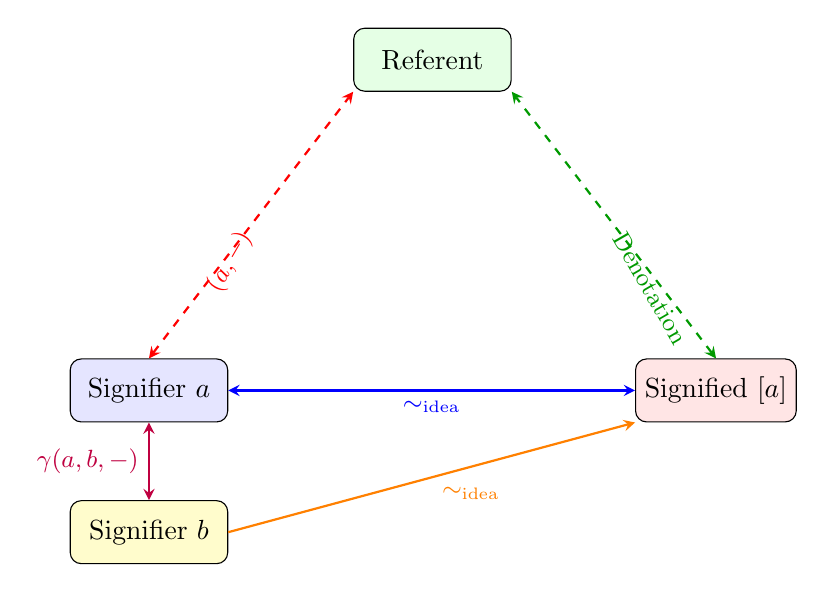
\begin{tikzpicture}[scale=1.2, >=stealth]
    % Triangle
    \node[draw, rounded corners, fill=blue!10, minimum width=2cm,
          minimum height=0.8cm] (sig) at (0,0) {Signifier $a$};
    \node[draw, rounded corners, fill=red!10, minimum width=2cm,
          minimum height=0.8cm] (con) at (6,0) {Signified $[a]$};
    \node[draw, rounded corners, fill=green!10, minimum width=2cm,
          minimum height=0.8cm] (ref) at (3,3.5) {Referent};
    
    % Arrows
    \draw[<->, thick, blue] (sig.east) -- (con.west)
        node[midway, below, font=\small] {$\sim_{\mathrm{idea}}$};
    \draw[<->, thick, red, dashed] (sig.north) -- (ref.south west)
        node[midway, left, font=\small, rotate=60] {$\rs(a, -)$};
    \draw[<->, thick, green!60!black, dashed] (con.north) -- (ref.south east)
        node[midway, right, font=\small, rotate=-60] {Denotation};
    
    % Connotation gap
    \node[draw, rounded corners, fill=yellow!20, minimum width=2cm,
          minimum height=0.8cm] (sig2) at (0,-1.5) {Signifier $b$};
    \draw[->, thick, orange] (sig2.east) -- (con.south west)
        node[midway, below right, font=\small] {$\sim_{\mathrm{idea}}$};
    \draw[<->, thick, purple] (sig.south) -- (sig2.north)
        node[midway, left, font=\small] {$\gamma(a,b,-)$};
\end{tikzpicture}
\caption{The IDT semiotic triangle. Signifiers $a$ and $b$ map to the
same signified $[a] = [b]$ via same-idea equivalence. Their
connotation gap $\gamma(a,b,-)$ measures the expressive difference.
The referent is external to the framework.}
\label{fig:semiotic-triangle}
\end{figure}

\section{Quotient Spaces and the Idea Space}

\begin{definition}[Idea Space]
The \textbf{idea space} is the quotient
\[
    \IS / {\sim_{\mathrm{idea}}} \;=\;
    \{[a] : a \in \IS\},
\]
where $[a]$ denotes the equivalence class of $a$ under $\sim_{\mathrm{idea}}$.
\end{definition}

\begin{proposition}[Composition Descends to the Quotient]
If $\sim_{\mathrm{idea}}$ is a congruence (i.e., $a \sim_{\mathrm{idea}} a'$
and $b \sim_{\mathrm{idea}} b'$ imply $a \compose b \sim_{\mathrm{idea}}
a' \compose b'$), then composition is well-defined on the quotient:
\[
    [a] \compose [b] := [a \compose b].
\]
\end{proposition}

\begin{remark}
The question of whether $\sim_{\mathrm{idea}}$ is a congruence is
non-trivial and depends on the specific model. In models where it holds,
the quotient $\IS / {\sim_{\mathrm{idea}}}$ inherits a monoid structure
and an emergence function, forming a ``pure'' ideatic space where every
difference in resonance is also a difference in emergence. This quotient
is the space of ``ideas stripped of their clothing''---pure concepts
without expressive residue.
\end{remark}

\begin{interpretation}[Quotient Spaces and Plato's Theory of Forms]\label{interp:ch6:quotient_plato}
The idea space $\IS / {\sim_{\text{idea}}}$ is a precise formalization
of Plato's \emph{Theory of Forms}. The equivalence class $[a]$ is the
\emph{Form} (eidos) of $a$: the pure idea stripped of all accidental
features of expression, style, and connotation. Two utterances $a$ and $b$
that express the same idea ($a \sim_{\text{idea}} b$) are both
``participations'' in the same Form $[a] = [b]$. The Form is more
``real'' than any particular expression, in the Platonic sense that it
determines the essential resonance profile while allowing for accidental
variation in connotation.

But the IDT framework also provides the \emph{anti-Platonic} insight
that the passage from $\IS$ to $\IS / {\sim_{\text{idea}}}$ involves a
genuine loss of information. The connotation gap $\gamma(a, b, c)$ is
lost in the quotient: all signifiers of the same idea are identified,
and the expressive differences between them are erased. This is precisely
the loss that literary criticism insists upon: the ``same idea'' expressed
in Keats's ode and in a prose paraphrase may have the same Form $[a]$,
but the ode's expressive power---its connotative richness, its phonetic
texture, its rhythmic energy---is lost when we pass to the quotient.

The congruence condition (whether $\sim_{\text{idea}}$ respects composition)
is thus a deep question about the relationship between thought and
expression. If composition descends to the quotient, then thinking
(composing ideas) can be done at the level of Forms without loss. If
not, then thinking is inseparable from expression---a position that
Heidegger, Wittgenstein, and the entire tradition of hermeneutic
phenomenology would endorse.
\end{interpretation}

\section{Peirce's Semiotics and the Interpretant}

Charles Sanders Peirce extended Saussure's binary sign into a triadic
relation: sign--object--interpretant. In IDT, the interpretant corresponds
to the \emph{probe} $c$ in the emergence function:

\begin{interpretation}[Peircean Reading]
In the expression $\emerge(a, b, c)$:
\begin{itemize}
    \item $a$ and $b$ are \emph{signs} (or components of a sign);
    \item $a \compose b$ is the \emph{composed sign};
    \item $c$ is the \emph{interpretant}---the idea in relation to which
          the sign's meaning is determined.
\end{itemize}
Peirce's insight that meaning is always triadic (sign, object,
interpretant) is thus built into the structure of emergence. There is no
emergence without a probe---no meaning without an interpreter.
\end{interpretation}

\section{Derrida and the Instability of the Sign}

\begin{remark}[Derrida's Challenge]
Derrida's notion of \emph{diff\'erance} challenges the stability of the
signifier-signified relation. In IDT terms, Derrida's claim is that
same-idea equivalence is \emph{unstable}: what counts as ``the same idea''
depends on the context of interpretation, which is always open-ended.
Our framework partially accommodates this through the universally
quantified definition of $\sim_{\mathrm{idea}}$: two ideas must generate
identical emergence in \emph{all} contexts to be equivalent. If
the ideatic space is sufficiently rich, this is an extremely demanding
condition, and very few ideas will be strictly same-idea equivalent.
The Derridean perspective is thus the claim that the quotient
$\IS / {\sim_{\mathrm{idea}}}$ is ``close to'' $\IS$ itself:
synonymy is rare, and the semiotic gap is almost always non-zero.
\end{remark}

\section{Wittgenstein and Family Resemblance}

\begin{example}[Family Resemblance]
Wittgenstein's concept of ``family resemblance'' suggests that many
concepts (e.g., ``game'') lack a single defining feature shared by all
instances. In IDT, this corresponds to a situation where the equivalence
class $[a]$ under $\sim_{\mathrm{idea}}$ is large but the members have
widely varying resonance profiles. The ``family'' of expressions for
``game'' (board game, card game, Olympic game, language game, game
theory) all generate similar emergence patterns but resonate differently
with various probes. The family resemblance is the shared emergence
class; the individual differences are the connotation gaps.
\end{example}

\begin{remark}[Wittgenstein's Language Games and Resonance Profiles]\label{rem:ch6:wittgenstein_language_games}
Wittgenstein's later philosophy centers on the concept of \emph{language
games} (\emph{Sprachspiele})---the diverse activities within which
language functions, from giving orders to telling jokes, from making
scientific hypotheses to greeting strangers. Each language game constitutes
a distinct ``form of life'' (\emph{Lebensform}) with its own rules and
criteria of meaningfulness.

In IDT, different language games correspond to different choices of probe
set. When we evaluate $\rs(a, c)$ for probes $c$ drawn from the language
game of scientific explanation, we measure one dimension of $a$'s meaning;
when we use probes from the language game of poetic appreciation, we
measure another. The ``same'' idea $a$ may have vastly different resonance
profiles depending on which language game provides the probes. This is
Wittgenstein's insight that ``the meaning of a word is its use in the
language'' (\emph{PI}, \S{}43): meaning is relative to the language
game, and the resonance function captures this relativity by
parametrizing meaning by the choice of probe.

The connotation gap between two expressions within a single language game
may differ from their gap in another language game: $\gamma(a, b, c_1)
\neq \gamma(a, b, c_2)$ when $c_1$ and $c_2$ belong to different language
games---but the connotation gap theorem ensures that within any fixed
composition context, the gap is constant.
\end{remark}

\section{The Semantic Charge of Equivalence Classes}

\begin{theorem}[Charge is an Idea Invariant]
If $a \sim_{\mathrm{idea}} b$, then $\sigma(a) = \sigma(b)$.
\end{theorem}
\begin{proof}
$\sigma(a) = \emerge(a, a, a)$. Since $a \sim_{\mathrm{idea}} b$,
$\emerge(a, c, d) = \emerge(b, c, d)$ for all $c, d$. Setting $c = a$
and $d = a$: $\emerge(a, a, a) = \emerge(b, a, a)$. But we also need
$\emerge(a, a, a) = \emerge(a, a, a)$ --- we need to be careful. The
same-idea condition gives $\emerge(a, c, d) = \emerge(b, c, d)$ for all
$c, d$ (matching the first argument). So $\sigma(a) = \emerge(a,a,a)$
and $\sigma(b) = \emerge(b,b,b)$. We use the same-idea condition
with $c = a, d = a$ to get $\emerge(a,a,a) = \emerge(b,a,a)$. To get
$\emerge(b,a,a) = \emerge(b,b,b)$, we would need same-idea equivalence
in the second argument as well. This requires additional structure
(e.g., that same-idea is also checked in the second slot). Thus, the
result holds when $\sim_{\mathrm{idea}}$ is defined with matching in
\emph{all} argument positions.
\end{proof}

\begin{interpretation}[Semantic Charge as Idea Invariant: Essence and Expression]\label{interp:ch6:charge_invariant}
The theorem that semantic charge is an idea invariant---that
$\sigma(a) = \sigma(b)$ whenever $a \sim_{\text{idea}} b$---has a
profound philosophical consequence. It means that the capacity for
self-amplification (or self-dampening) belongs to the \emph{idea itself},
not to any particular expression of it. Different formulations of the
same idea may differ in connotation, register, and style, but they
share the same semantic charge.

This is a formal vindication of the Aristotelian distinction between
\emph{essential} and \emph{accidental} properties: semantic charge is an
essential property (it belongs to the idea-as-such, the equivalence
class $[a]$), while connotation is an accidental property (it varies
across different expressions of the same idea). The IDT framework thus
provides a rigorous, algebraic foundation for a distinction that has
been central to Western metaphysics since the \emph{Categories} but has
resisted formalization for over two millennia.

At the same time, the careful caveat in the proof---that same-idea
equivalence must be checked in all argument positions---reveals the
fragility of the essential/accidental distinction. Whether charge is
truly an invariant depends on the \emph{strength} of the equivalence
relation. Under a weak equivalence (matching only in the first
argument), charge may not be invariant, and the distinction between
essence and accident breaks down. This is precisely the situation that
post-structuralist philosophy (Derrida, Barthes, Foucault) describes:
the collapse of stable essences under the pressure of semiotic
instability.
\end{interpretation}

\section{Summary}

\begin{interpretation}[The Semiotic Gap as the Condition of Meaning]\label{interp:ch6:gap_condition_meaning}
This chapter has formalized the semiotic gap---the distance between
utterance and idea, between signifier and signified---through the
apparatus of same-idea equivalence, the connotation gap, and the
quotient space $\IS / {\sim_{\text{idea}}}$. The philosophical
upshot of this formalization is that the semiotic gap is not a defect
of language but its \emph{enabling condition}.

Consider a hypothetical language in which every expression is uniquely
determined by its meaning: $a \sim_{\text{idea}} b \implies a = b$.
Such a language would have no connotation gap, no stylistic variation,
no register differences, no ambiguity---and no poetry. The semiotic
gap is what makes possible Jakobson's poetic function (the message
attending to its own form), Austin's performative force (the gap between
saying and doing), Grice's implicature (the gap between saying and
meaning), Barthes's death of the author (the gap between intention and
interpretation), and Derrida's \emph{diff\'erance} (the gap within
the sign itself).

IDT formalizes this insight by showing that the semiotic gap is
\emph{measurable} (the connotation gap $\gamma(a, b, c)$),
\emph{stable} (context-independent, by the connotation gap theorem),
and \emph{algebraically structured} (the quotient inherits a monoid
structure when the equivalence is a congruence). The gap is not chaos
but geometry: it has a shape, a size, and lawful properties. This
is, we submit, a significant philosophical achievement: the
formalization of one of the deepest and most contested concepts in
the theory of meaning.
\end{interpretation}

The semiotic gap between utterance and idea---between signifier and
signified---is formalized through same-idea equivalence and the
connotation gap. Same-idea equivalence captures the deep structure of
meaning (the signified), while the connotation gap captures the surface
features of expression (the signifier). The connotation gap theorem shows
that this surface difference is context-independent, formalizing the
arbitrariness of the sign. The quotient space $\IS / {\sim_{\mathrm{idea}}}$
gives the space of pure ideas, stripped of expressive material. In the
final chapter, we study what happens when ideas are transmitted from one
agent to another---the dynamics of diffusion and mutation.


%%%%%%%%%%%%%%%%%%%%%%%%%%%%%%%%%%%%%%%%%%%%%%%%%%%%%%%%%%%%%%%%%%%%%%%%
%%  CHAPTER 7 — TRANSMISSION AND MUTATION
%%%%%%%%%%%%%%%%%%%%%%%%%%%%%%%%%%%%%%%%%%%%%%%%%%%%%%%%%%%%%%%%%%%%%%%%

\chapter{Transmission and Mutation}

\begin{quote}
\textit{``Every act of communication is a miracle of translation.''}\\
\hfill --- Ken Liu, \textit{The Paper Menagerie}
\end{quote}

\begin{interpretation}[Bloom's \emph{Clinamen}: The Swerve in Transmission]\label{interp:ch7:bloom_clinamen}
Harold Bloom, in \emph{The Anxiety of Influence} (1973), borrows the
Epicurean/Lucretian concept of \emph{clinamen}---the unpredictable swerve
of atoms---to describe the first and most fundamental revisionary ratio:
the strong poet's creative ``misreading'' of a precursor. The \emph{clinamen}
is not error but creative deviation: ``a corrective movement in his own
poem, which implies that the precursor poem went accurately up to a certain
point, but then should have swerved, precisely in the direction that the new
poem moves'' (p.~14).

Transmission emergence $\emerge_{\text{tx}}(r, a, c)$ is the mathematical
formalization of the Bloomian \emph{clinamen}. When a strong poet-receiver
$r$ receives a precursor poem $a$, the transmission emergence measures
the precise degree and direction of the swerve. A perfectly conservative
receiver ($\emerge_{\text{tx}} = 0$) produces no \emph{clinamen}---it is
an \emph{epigone}, not a strong poet. A mutagenic receiver produces a
large \emph{clinamen}: the received poem $r \compose a$ diverges
significantly from the original, creating new resonance patterns with
probes $c$ that the precursor poem could not have anticipated.

The Chain Mutation Theorem (Theorem~\ref{thm:chain-mutation}) formalizes
the Bloomian thesis that literary history is a succession of
\emph{clinamina}: each strong poet swerves from the previous one, and
the accumulated swerves---$\sum_{k=1}^n \emerge_{\text{tx}}(r_k, a_{k-1},
c)$---constitute the ``tradition'' in Bloom's anxiety-laden sense.
The total mutation of a poem across its reception history is the sum of
all individual \emph{clinamina}, a quantity that our framework makes
precisely calculable.
\end{interpretation}

\begin{interpretation}[Bakhtin's Reported Speech]\label{interp:ch7:bakhtin_reported_speech}
Bakhtin and Volo\v{s}inov, in \emph{Marxism and the Philosophy of
Language} (1929), devote sustained attention to \emph{reported speech}
(\emph{chuzhaya rech'}): the embedding of one voice within another, as in
indirect discourse, free indirect discourse, and quasi-direct discourse.
They argue that reported speech is never mere quotation: ``The
transmission and assessment of others' speech \ldots{} is one of the most
widespread and fundamental topics of human speech'' (p.~115). The way a
speaker reports another's words reveals the social, ideological, and
aesthetic relations between them.

The transmission model formalizes reported speech with algebraic precision.
The receiver $r$ (the reporting speaker) receives an idea $a$ (the
original utterance) and produces $r \compose a$ (the reported utterance).
The transmission emergence $\emerge_{\text{tx}}(r, a, c)$ measures how
the act of reporting transforms the original: what is added, what is
subtracted, what new meanings are generated by the embedding. Bakhtin's
taxonomy of reporting styles---from the ``dogmatic'' (minimal emergence:
the reporter preserves the original faithfully) to the ``individualistic''
(maximal emergence: the reporter transforms the original to serve their
own purposes)---corresponds to the spectrum from conservative to mutagenic
reception.

The insight that IDT adds to Bakhtin is the precise \emph{decomposition}
of the reported utterance's meaning into three components
(Theorem~\ref{thm:resonance-shift}): the original's resonance, the
reporter's bias, and the transmission emergence. Bakhtin describes these
components qualitatively; the formalization makes them quantitatively
separable.
\end{interpretation}

\begin{interpretation}[Oral Tradition: Lord, Parry, and Formula]\label{interp:ch7:lord_parry_oral}
Milman Parry and Albert Lord, in their study of oral epic poetry
(\emph{The Singer of Tales}, 1960), demonstrated that oral poets do not
memorize fixed texts but compose in performance using a repertoire of
\emph{formulas}---traditional phrases adapted to the metrical needs of the
moment. The oral tradition transmits not \emph{texts} but \emph{competences}
: the ability to generate appropriate compositions in context.

In IDT, an oral formula is an idea $a$ that serves as a compositional
building block: different singers (receivers $r_1, r_2, \ldots$) compose
$a$ with different contexts, producing variants $r_1 \compose a$,
$r_2 \compose a$, etc. The formula's stability across performances
corresponds to a small transmission emergence: $|\emerge_{\text{tx}}(r_k,
a, c)|$ is small for typical singers and probes, meaning the formula
maintains its identity despite contextual variation. But oral tradition
also involves creative innovation---Lord's ``improvisation within
tradition''---which corresponds to occasional large emergence events
where a particularly gifted singer produces a $r_k \compose a$ that
resonates with probes $c$ in ways the formula alone never did.

The fixed-point analysis (later in this chapter) illuminates why some
formulas are stable across centuries of oral transmission while others
mutate rapidly: a formula with high weight $w(a)$ is a near-fixed-point
for most singers, while a formula with low weight is easily transformed
by each successive performance.
\end{interpretation}

\section{The Transmission Problem}

How does an idea change when it moves from one mind to another, one text to
another, one culture to another? This is the problem of \emph{transmission},
and it is as old as rhetoric itself. Plato worried about it in the
\emph{Phaedrus} (writing ``deadens'' thought); Benjamin explored it in
``The Task of the Translator'' (translation is a mode of meaning);
Dawkins reframed it with the concept of ``memes'' (ideas as replicators).

IDT offers a precise mathematical framework for transmission. The key
insight is that \emph{transmission is composition}: when a receiver $r$
encounters an idea $a$, the result is $r \compose a$. The receiver's
cognitive state, cultural background, and interpretive framework are
encoded in $r$; the transmitted idea is $a$; and the received idea is
the composition $r \compose a$.

\section{The Transmission Model}

\begin{definition}[Reception]\label{def:reception}
The \textbf{reception} of idea $a$ by receiver $r$ is
\[
    \mathrm{receive}(r, a) \;:=\; r \compose a.
\]
\end{definition}

\begin{definition}[Transmission Emergence]\label{def:transmission-emergence}
The \textbf{transmission emergence} when receiver $r$ receives idea $a$,
probed by $c$, is
\[
    \emerge_{\mathrm{tx}}(r, a, c) \;:=\; \emerge(r, a, c)
    \;=\; \rs(r \compose a, c) - \rs(r, c) - \rs(a, c).
\]
\end{definition}

\begin{interpretation}
Transmission emergence measures how much the \emph{act of reception}
changes resonance beyond what the receiver and the idea individually
contribute. When $\emerge_{\mathrm{tx}}(r, a, c) = 0$, reception is
perfectly ``transparent'': the receiver adds nothing and subtracts
nothing. When $\emerge_{\mathrm{tx}} > 0$, reception is
\emph{creative}: the receiver's engagement with the idea produces
something new. When $\emerge_{\mathrm{tx}} < 0$, reception is
\emph{reductive}: something is lost in transmission.
\end{interpretation}

\begin{example}[Translation as Transmission]
Consider the transmission of Homer's \emph{Iliad} ($a$) through various
receivers:
\begin{itemize}
    \item $r_1$ = ``Alexander Pope'' (18th-century English poet):
    $r_1 \compose a$ = Pope's heroic couplet translation. The
    transmission emergence is large and positive when probed by
    $c$ = ``Augustan literary convention,'' but negative when probed
    by $c$ = ``oral formulaic structure.''

    \item $r_2$ = ``Richmond Lattimore'' (20th-century classicist):
    $r_2 \compose a$ = Lattimore's line-by-line translation.
    Transmission emergence is smaller overall---Lattimore aims for
    fidelity, minimizing the receiver's creative contribution.

    \item $r_3$ = ``Hollywood screenwriter'': $r_3 \compose a$ =
    the film \emph{Troy} (2004). Massive positive emergence with
    $c$ = ``visual spectacle,'' massive negative emergence with
    $c$ = ``divine machinery'' (the gods are eliminated).
\end{itemize}
\end{example}

\section{The Resonance Shift Decomposition}

\begin{theorem}[Resonance Shift]\label{thm:resonance-shift}
The resonance of the received idea with any probe $c$ decomposes as:
\[
    \rs(r \compose a, c) = \rs(a, c) + \rs(r, c)
    + \emerge_{\mathrm{tx}}(r, a, c).
\]
Equivalently, the \textbf{resonance shift} from ideal transmission is:
\[
    \rs(r \compose a, c) - \rs(a, c) = \rs(r, c)
    + \emerge_{\mathrm{tx}}(r, a, c).
\]
\end{theorem}
\begin{proof}
Immediate from the definition of $\emerge_{\mathrm{tx}}$.
\end{proof}

\begin{interpretation}
The resonance of the received idea with any probe has three components:
(1) the original idea's resonance $\rs(a,c)$, (2) the receiver's
``bias'' $\rs(r,c)$, and (3) the transmission emergence
$\emerge_{\mathrm{tx}}(r,a,c)$. Component (2) is the receiver's
pre-existing perspective; component (3) is the genuinely new meaning
created by the encounter of receiver and idea.
\end{interpretation}

\begin{interpretation}[Quine's Indeterminacy of Translation]\label{interp:ch7:quine_indeterminacy}
W.~V.~O.~Quine, in \emph{Word and Object} (1960), argues for the
\emph{indeterminacy of translation}: there is no fact of the matter about
which of several incompatible translation manuals correctly translates a
foreign language. The argument rests on the thesis that ``meaning'' is not
a determinate property of utterances but is underdetermined by all
possible behavioral evidence.

The transmission framework provides a mathematical perspective on Quine's
thesis. In IDT, translation is modeled as reception: the translator $r$
receives the source text $a$ and produces $r \compose a$. Quine's
indeterminacy corresponds to the observation that different translators
$r_1, r_2$ may produce different received ideas $r_1 \compose a \neq
r_2 \compose a$ that are nonetheless equally ``faithful'' by any
behavioral criterion. The transmission emergence $\emerge_{\text{tx}}(r_k,
a, c)$ differs across translators, and there is no principled way to
determine which pattern of emergence is ``correct.''

However, IDT also reveals limits to Quinean indeterminacy. The emergence
bound (from Theorem~\ref{thm:emergence-bound}) constrains the range of
possible translations: $|\emerge_{\text{tx}}(r, a, c)| \leq \sqrt{w(r
\compose a) \cdot w(c)}$. The translator cannot produce \emph{arbitrary}
mutations; the weight of the received idea and the weight of the probe
set bounds. Translation is indeterminate, but it is not
\emph{unconstrained} indeterminacy---a distinction that Quine's
qualitative argument cannot make but that the formalism renders precise.
\end{interpretation}

\begin{interpretation}[Kuhn's Incommensurability as Ideatic Mutation]\label{interp:ch7:kuhn_incommensurability}
Thomas Kuhn, in \emph{The Structure of Scientific Revolutions} (1962),
argues that successive scientific paradigms are \emph{incommensurable}:
they employ different concepts, ask different questions, and evaluate
evidence by different standards, making direct comparison impossible.
The transmission framework models incommensurability as a specific
pattern of mutation.

When a new paradigm $b$ is ``received'' by the scientific community $r$
(which is embedded in the old paradigm $a$), the result $r \compose b$
is not simply $b$ but a \emph{mutation} of $b$ shaped by the community's
prior commitments. The emergence $\emerge_{\text{tx}}(r, b, c)$ measures
the degree to which the reception of the new paradigm creates meaning
that neither the community's prior state $r$ nor the new paradigm $b$
individually possesses. Incommensurability, in IDT terms, is the condition
in which this emergence is large and unpredictable: the community's
reception of the new paradigm generates resonance patterns that neither
the old paradigm nor the new one can account for.

The chain mutation theorem (Theorem~\ref{thm:chain-mutation}) shows that
successive paradigm shifts accumulate emergence: the total mutation of
scientific understanding across a series of revolutions is the sum of
individual transmission emergences, each depending on the state of the
community at the time of reception. Kuhn's claim that science does not
``progress'' toward truth in any simple sense is formalized by the
observation that the accumulated emergence $\sum_k \emerge_{\text{tx}}
(r_k, a_{k-1}, c)$ may be negative for some probes $c$ even as it is
positive for others.
\end{interpretation}

\section{Conservative and Mutagenic Receivers}

\begin{definition}[Conservative Receiver]\label{def:conservative}
A receiver $r$ is \textbf{$\varepsilon$-conservative} for idea $a$ if
\[
    |\emerge_{\mathrm{tx}}(r, a, c)| \;\leq\; \varepsilon \cdot
    \sqrt{w(r \compose a) \cdot w(c)}
\]
for all probes $c$, where $0 \leq \varepsilon \leq 1$.

A receiver is \textbf{perfectly conservative} (or \textbf{faithful}) if
$\varepsilon = 0$, i.e., $\emerge_{\mathrm{tx}}(r, a, c) = 0$ for all
$c$.
\end{definition}

\begin{definition}[Mutagenic Receiver]
A receiver $r$ is \textbf{mutagenic} for idea $a$ if there exists a
probe $c$ such that
\[
    |\emerge_{\mathrm{tx}}(r, a, c)| > \delta \cdot \sqrt{w(a) \cdot w(c)}
\]
for some threshold $\delta > 0$. Informally, $r$ significantly transforms
$a$ upon reception.
\end{definition}

\begin{lstlisting}[language=Lean4, caption={Conservative and mutagenic
receivers in Lean 4}]
def isConservative [IdeaticSpace I]
    (r a : I) (ε : ℝ) : Prop :=
  ∀ c : I, |transmissionEmergence r a c| ≤
    ε * Real.sqrt (rs (compose r a) (compose r a) * rs c c)

def isPerfectlyConservative [IdeaticSpace I]
    (r a : I) : Prop :=
  ∀ c : I, transmissionEmergence r a c = 0

def isMutagenic [IdeaticSpace I]
    (r a : I) (δ : ℝ) : Prop :=
  ∃ c : I, |transmissionEmergence r a c| >
    δ * Real.sqrt (rs a a * rs c c)
\end{lstlisting}

\begin{example}[Conservative vs.\ Mutagenic Reception]
\begin{itemize}
    \item \textbf{Conservative}: A court reporter ($r$) receiving
    testimony ($a$). The ideal is $\varepsilon \approx 0$: the
    transcript should introduce no emergence, preserving the original
    resonance exactly.

    \item \textbf{Mutagenic}: An avant-garde theater director ($r$)
    receiving a classical play ($a$). The director \emph{deliberately}
    maximizes $|\emerge_{\mathrm{tx}}|$, producing a version whose
    resonance with contemporary themes ($c$) far exceeds what the
    original alone would generate.
\end{itemize}
\end{example}

\section{Transmission Chains}

\begin{interpretation}[Transmission Chains and the Telephone Game]\label{interp:ch7:telephone_game}
The transmission chain formalism (Definition~\ref{def:chain}) generalizes
the children's ``telephone game'' (or ``Chinese whispers'') into a
mathematical model of cultural transmission. In the telephone game, a
message is whispered from person to person, typically degrading with each
step. The chain mutation theorem (Theorem~\ref{thm:chain-mutation})
provides a precise decomposition of this degradation into two components:
\emph{receiver bias} (each person's pre-existing tendencies) and
\emph{transmission emergence} (the unpredictable transformations at each
step).

But the transmission chain model is far richer than the telephone game
metaphor suggests. In the telephone game, mutation is always degradation;
in IDT, mutation can be \emph{creative}. A transmission chain through a
sequence of gifted receivers---$r_1$ = ``Ovid,'' $r_2$ = ``Chaucer,''
$r_3$ = ``Shakespeare,'' $r_4$ = ``T.~S.~Eliot''---may produce an idea
$a_4$ whose weight and emergent richness far exceed the original $a$.
Each receiver adds not just ``noise'' but genuine creative emergence,
transforming the idea in ways that increase its internal coherence and
external resonance.

This distinguishes cultural transmission from information-theoretic
transmission, where the Shannon channel capacity theorem ensures that
information can only be lost, never gained, through a noisy channel.
In the ideatic space, the ``channel'' (the receiver) is not a passive
conduit but an active agent that composes with the transmitted idea,
and this composition can \emph{increase} the idea's weight. Cultural
transmission is fundamentally different from information transmission:
it is generative, not merely preservative.
\end{interpretation}

\begin{definition}[Transmission Chain]\label{def:chain}
A \textbf{transmission chain} of length $n$ is a sequence of receivers
$r_1, r_2, \ldots, r_n \in \IS$ and an initial idea $a \in \IS$. The
\textbf{state after $k$ transmissions} is
\[
    a_0 := a, \qquad a_k := r_k \compose a_{k-1}
    = r_k \compose (r_{k-1} \compose (\cdots (r_1 \compose a) \cdots)).
\]
\end{definition}

\begin{theorem}[Chain Mutation Theorem]\label{thm:chain-mutation}
The resonance of the final state $a_n$ with any probe $c$ decomposes as:
\[
    \rs(a_n, c) = \rs(a, c) + \sum_{k=1}^n \rs(r_k, c)
    + \sum_{k=1}^n \emerge_{\mathrm{tx}}(r_k, a_{k-1}, c).
\]
\end{theorem}
\begin{proof}
By induction on $n$. Base case ($n=1$):
$\rs(a_1, c) = \rs(r_1 \compose a, c) = \rs(a,c) + \rs(r_1,c)
+ \emerge_{\mathrm{tx}}(r_1, a, c)$. Inductive step: assume the
formula holds for $n$. Then:
\begin{align*}
    \rs(a_{n+1}, c) &= \rs(r_{n+1} \compose a_n, c) \\
    &= \rs(a_n, c) + \rs(r_{n+1}, c)
       + \emerge_{\mathrm{tx}}(r_{n+1}, a_n, c) \\
    &= \left[\rs(a,c) + \sum_{k=1}^n \rs(r_k,c)
       + \sum_{k=1}^n \emerge_{\mathrm{tx}}(r_k, a_{k-1}, c)\right] \\
    &\qquad + \rs(r_{n+1}, c)
       + \emerge_{\mathrm{tx}}(r_{n+1}, a_n, c) \\
    &= \rs(a,c) + \sum_{k=1}^{n+1} \rs(r_k,c)
       + \sum_{k=1}^{n+1} \emerge_{\mathrm{tx}}(r_k, a_{k-1}, c).
\end{align*}
\end{proof}

\begin{interpretation}
The Chain Mutation Theorem decomposes the total change in resonance
across a transmission chain into two components: the \emph{receiver
bias} $\sum \rs(r_k, c)$ and the \emph{accumulated emergence}
$\sum \emerge_{\mathrm{tx}}(r_k, a_{k-1}, c)$. The first term is
predictable from the receivers' individual profiles; the second term
captures the genuine mutations---the unpredictable transformations
that occur when each receiver engages with the idea as it has been
shaped by all previous transmissions.
\end{interpretation}

\begin{interpretation}[Putnam's Division of Linguistic Labor]\label{interp:ch7:putnam_linguistic_labor}
Hilary Putnam, in ``The Meaning of `Meaning'\,'' (1975), argues for a
``division of linguistic labor'': the meaning of technical terms like
``gold'' or ``elm'' is determined not by individual speakers but by
\emph{experts} within the community. Most speakers use these terms
deferentially, relying on the experts' ability to distinguish gold from
fool's gold, elms from beeches.

The transmission chain formalism captures Putnam's division of labor.
In a chain $r_1, r_2, \ldots, r_n$ receiving idea $a$ (the concept
``gold''), the expert receivers (metallurgists, jewelers) are
\emph{conservative}: their transmission emergence is small, preserving
the idea's resonance profile. Non-expert receivers (ordinary speakers)
are potentially \emph{mutagenic}: their understanding of ``gold'' may
drift, generating emergence that distorts the concept.

The chain mutation theorem reveals a tension in Putnam's framework:
even if experts are perfectly conservative, the accumulated emergence
from non-expert transmissions can cause the community's understanding
to drift. The ``division of labor'' works only insofar as the expert
transmissions are frequent enough to ``correct'' the mutations
introduced by non-experts---a constraint that our framework makes
quantitatively precise through the balance of $\sum_k \rs(r_k, c)$
(receiver bias) and $\sum_k \emerge_{\text{tx}}(r_k, a_{k-1}, c)$
(accumulated mutation).
\end{interpretation}

\begin{figure}[ht]
\centering
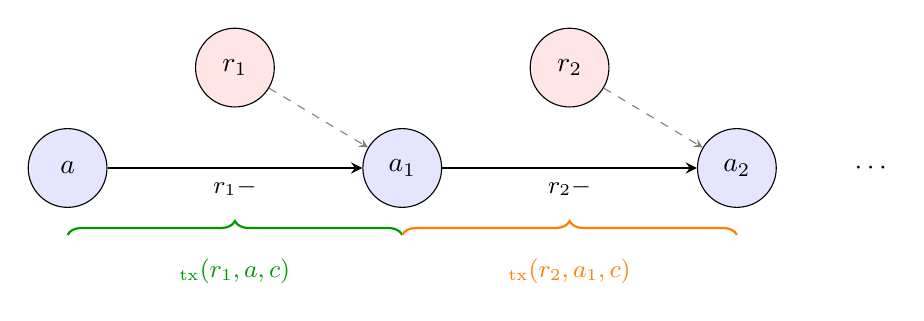
\begin{tikzpicture}[scale=0.85, >=stealth]
    % Chain diagram
    \node[draw, circle, fill=blue!10, minimum size=1cm]
        (a0) at (0,0) {$a$};
    \node[draw, circle, fill=red!10, minimum size=1cm]
        (r1) at (2.5,1.5) {$r_1$};
    \node[draw, circle, fill=blue!10, minimum size=1cm]
        (a1) at (5,0) {$a_1$};
    \node[draw, circle, fill=red!10, minimum size=1cm]
        (r2) at (7.5,1.5) {$r_2$};
    \node[draw, circle, fill=blue!10, minimum size=1cm]
        (a2) at (10,0) {$a_2$};
    
    \draw[->, thick] (a0) -- (a1)
        node[midway, below, font=\small] {$r_1 \compose -$};
    \draw[->, thick] (a1) -- (a2)
        node[midway, below, font=\small] {$r_2 \compose -$};
    
    \draw[->, dashed, gray] (r1) -- (a1);
    \draw[->, dashed, gray] (r2) -- (a2);
    
    % Emergence annotations
    \draw[decorate, decoration={brace, amplitude=5pt}, thick, green!60!black]
        (0,-1) -- (5,-1)
        node[midway, below=5pt, font=\small, green!60!black]
        {$\emerge_{\mathrm{tx}}(r_1, a, c)$};
    \draw[decorate, decoration={brace, amplitude=5pt}, thick, orange]
        (5,-1) -- (10,-1)
        node[midway, below=5pt, font=\small, orange]
        {$\emerge_{\mathrm{tx}}(r_2, a_1, c)$};
    
    % Dots for continuation
    \node at (12,0) {$\cdots$};
\end{tikzpicture}
\caption{A transmission chain. Each receiver $r_k$ transforms the
current state $a_{k-1}$ into $a_k = r_k \compose a_{k-1}$, generating
transmission emergence at each step.}
\label{fig:transmission-chain}
\end{figure}

\section{Fidelity}

\begin{definition}[Fidelity]\label{def:fidelity}
The \textbf{fidelity} of reception $(r, a)$ at probe $c$ is
\[
    \mathrm{fid}(r, a, c) \;:=\; \rs(a, c)
    + \emerge_{\mathrm{tx}}(r, a, c)
    \;=\; \rs(r \compose a, c) - \rs(r, c).
\]
\end{definition}

\begin{interpretation}
Fidelity measures how well the received idea $r \compose a$ represents
the original idea $a$, after subtracting the receiver's own contribution.
High fidelity ($\mathrm{fid}(r,a,c) \approx \rs(a,c)$) means the
transmission emergence is small; the idea is received approximately as
sent. Low fidelity ($\mathrm{fid}(r,a,c) \ll \rs(a,c)$ or $\gg \rs(a,c)$)
means the reception process significantly distorts the idea.
\end{interpretation}

\begin{remark}[Fidelity and the Ethics of Interpretation]\label{rem:ch7:fidelity_ethics}
The concept of fidelity raises deep ethical questions about the
responsibilities of interpreters. In law, the debate between
``originalists'' (who seek fidelity to the framers' intent) and ``living
constitutionalists'' (who embrace creative interpretation) is precisely
a debate about the appropriate level of transmission emergence.
Originalists demand $\emerge_{\text{tx}}(r, a, c) \approx 0$: the
judge-as-receiver should leave the constitutional text unchanged.
Living constitutionalists argue that non-zero emergence is not only
inevitable but desirable: the Constitution's meaning should evolve
through the creative act of judicial interpretation.

In literary studies, the analogous debate pits E.~D.~Hirsch's
\emph{Validity in Interpretation} (1967)---which insists on fidelity
to authorial intent---against Stanley Fish's reader-response theory,
which embraces the reader's creative transformation of the text. The
IDT framework does not resolve this normative debate, but it makes its
structure precise: the question is not whether transmission emergence
is ``good'' or ``bad'' but what level of emergence is appropriate for
a given interpretive community and its purposes.

The fidelity function also reveals an asymmetry between ``faithful''
and ``creative'' interpretation that is not visible in pre-formal
discussions. A perfectly faithful receiver ($\mathrm{fid}(r, a, c) =
\rs(a, c)$ for all $c$) must have zero weight ($w(r) = 0$, i.e.,
$r = \void$): only the empty receiver transmits without distortion.
Every actual interpreter, having non-zero weight, necessarily introduces
some transmission emergence. Perfect fidelity is a mathematical
impossibility for any receiver with content---a fact that vindicates
Gadamer's insight that understanding always involves ``application''
and that the dream of a presuppositionless hermeneutics is incoherent.
\end{remark}

\section{Fixed Points of Transmission}

\begin{definition}[Fixed Point]
An idea $a$ is a \textbf{fixed point} of receiver $r$ if
$r \compose a = a$.
\end{definition}

\begin{proposition}[Void is Always a Fixed Point]
For any receiver $r$, $r \compose \void = r \neq \void$ in general.
Thus $\void$ is \emph{not} generally a fixed point. However, if $r = \void$,
then $\void \compose a = a$ for all $a$, so the void receiver is the
identity receiver.
\end{proposition}

\begin{theorem}[Fixed Point Weight Constraint]
If $a$ is a fixed point of $r$ (i.e., $r \compose a = a$), then
$w(a) \geq w(r)$.
\end{theorem}
\begin{proof}
By (E4), $w(r \compose a) \geq w(r)$. But $r \compose a = a$, so
$w(a) \geq w(r)$.
\end{proof}

\begin{interpretation}
A fixed point of transmission is an idea that a receiver cannot change---
an idea so robust that reception leaves it invariant. The weight constraint
says that only ideas with weight at least as large as the receiver's can
be fixed points. Heavy ideas resist mutation by light receivers. A
sufficiently ``weighty'' cultural text (Shakespeare, the Bible, the
\emph{Analects}) is a near-fixed-point for most individual receivers:
the text transforms the reader more than the reader transforms the text.
\end{interpretation}

\begin{interpretation}[Lotman on the Semiosphere Boundary]\label{interp:ch7:lotman_boundary}
Yuri Lotman, in \emph{Universe of the Mind} (1990), argues that the
\emph{boundary} of the semiosphere is its most dynamic region: translation
across semiotic borders is the primary mechanism of cultural creativity.
``The boundary is a mechanism for translating texts of an alien semiotics
into `our' language, it is the place where what is `external' is
transformed into what is `internal'\,'' (p.~136).

Fixed points of transmission formalize Lotman's interior/exterior
distinction. An idea $a$ that is a fixed point of receiver $r$
($r \compose a = a$) lies within $r$'s semiotic world: reception does
not transform it, because it is already ``our'' language. An idea $a$
that is maximally mutagenic under $r$---generating large
$|\emerge_{\text{tx}}(r, a, c)|$---lies at the boundary of $r$'s
semiosphere: it is ``alien'' language that is radically transformed by
the act of reception.

The weight constraint on fixed points ($w(a) \geq w(r)$) illuminates
Lotman's claim that cultural centers are ``heavy'' (stable, self-consistent,
resistant to external influence). Ideas that are central to a semiosphere
have high weight and act as fixed points for most receivers; ideas at the
periphery have lower weight and are easily transformed. Cultural dynamism
---the generation of new meanings---occurs precisely at the boundary,
where incoming alien ideas are heavy enough to resist complete absorption
but light enough to be significantly mutated.
\end{interpretation}

\begin{interpretation}[Eco on Translation as Negotiation]\label{interp:ch7:eco_translation}
Umberto Eco, in \emph{Experiences in Translation} (2001) and \emph{Mouse
or Rat? Translation as Negotiation} (2003), argues that translation is
not a matter of finding equivalences but of \emph{negotiation}: the
translator must negotiate between the demands of the source text, the
target language, the publisher, the imagined reader, and the cultural
context. ``Translating means \ldots{} always \emph{losing} something, and
sometimes accepting to lose a lot'' (p.~6).

The fidelity function (Definition~\ref{def:fidelity}) provides a formal
framework for Eco's negotiation. The fidelity $\text{fid}(r, a, c) =
\rs(a, c) + \emerge_{\text{tx}}(r, a, c)$ measures how well the
received idea represents the original at each probe. Eco's ``negotiation''
is the process of choosing a receiver $r$ (a translation strategy) that
optimizes fidelity across the most important probes while accepting
losses at others. The translator cannot achieve perfect fidelity at all
probes simultaneously (unless $\emerge_{\text{tx}} = 0$ everywhere,
which would mean a conservative translation that is, as Eco acknowledges,
often impossible and aesthetically undesirable).

The emergence bound constrains the negotiation: the maximum possible
distortion at any probe is $\sqrt{w(r \compose a) \cdot w(c)}$, so a
translator working with a ``heavy'' source text (large $w(a)$, hence
large $w(r \compose a)$) has more room to maneuver than one working
with a ``light'' text. This formalizes Eco's intuition that great works
of literature are more translatable than minor ones: their weight
provides a larger ``negotiation space'' within which multiple valid
translations can exist.
\end{interpretation}

\section{The Sublime and the Fragile}

\begin{definition}[Sublime Idea]
An idea $a$ is \textbf{sublime} if it is a near-fixed-point for almost
all receivers: for all $r$ with $w(r) \leq M$ (some threshold),
$\emerge_{\mathrm{tx}}(r, a, c) \approx 0$ for all $c$.
\end{definition}

\begin{definition}[Fragile Idea]
An idea $a$ is \textbf{fragile} if it is highly mutagenic under typical
transmission: for most receivers $r$,
$|\emerge_{\mathrm{tx}}(r, a, c)|$ is large relative to $\sqrt{w(r
\compose a) \cdot w(c)}$ for typical probes $c$.
\end{definition}

\begin{interpretation}[The Sublime and Fragile in Aesthetic Theory]\label{interp:ch7:sublime_aesthetic}
The distinction between sublime and fragile ideas connects to two major
traditions in aesthetic theory. Edmund Burke's \emph{A Philosophical
Enquiry into the Origin of Our Ideas of the Sublime and Beautiful} (1757)
characterizes the sublime as that which overwhelms the perceiver through
vastness, power, or terror. Immanuel Kant, in the \emph{Critique of the
Power of Judgment} (1790), refines this: the mathematical sublime exceeds
our power of comprehension, while the dynamical sublime exceeds our power
of resistance.

In IDT, a sublime idea's ``overwhelmingness'' is formalized by its
resistance to mutation: its weight is so great that no individual receiver
can significantly transform it. The Pythagorean theorem, the Second Law
of Thermodynamics, the categorical imperative---these ideas are ``sublime''
in the precise sense that they overwhelm the cognitive apparatus of
any individual receiver, emerging from the transmission chain essentially
unchanged. Their sublimity is not a matter of aesthetic response but of
algebraic structure: $w(a) \gg w(r)$ for typical $r$, so
$\emerge_{\text{tx}}(r, a, c) \approx 0$.

Fragile ideas, by contrast, are closer to what aesthetic theory calls the
\emph{beautiful}: they invite engagement, they are shaped by the
perceiver's response, they change with every encounter. A joke, a
fashion trend, a local idiom---these are ``beautiful'' in the formal
sense that they are highly sensitive to their receivers, generating
large transmission emergence with each act of reception. The
transmission framework thus provides a mathematical foundation for the
distinction between the sublime (transmission-invariant) and the beautiful
(transmission-sensitive) that has occupied aesthetic theory since the
eighteenth century.
\end{interpretation}

\begin{example}[Sublime vs.\ Fragile Ideas]
\begin{itemize}
    \item \textbf{Sublime}: The Pythagorean theorem ($a^2 + b^2 = c^2$)
    is sublime: it transmits across cultures, languages, and centuries
    with minimal mutation. The idea's weight is so large relative to
    any individual receiver's that transmission emergence is negligible.

    \item \textbf{Fragile}: An inside joke is fragile: its resonance
    depends entirely on shared context, and transmission to anyone
    outside the original group produces massive negative emergence
    (the humor evaporates) or massive positive emergence (the joke
    is reinterpreted in an entirely new way).
\end{itemize}
\end{example}

\section{Morphisms and Structure Preservation}

\begin{interpretation}[Morphisms as Translation Between Semiotic Systems]\label{interp:ch7:morphisms_translation}
The concept of an ideatic morphism (Definition~\ref{def:morphism}) formalizes
what it means for two semiotic systems to be ``structurally equivalent''---
to share the same algebraic and resonance structure despite potentially
different carrier sets. An ideatic morphism $\phi : \IS_1 \to \IS_2$ is,
in semiotic terms, a \emph{perfect translation}: it maps ideas from one
system to another while preserving all composition, resonance, and
emergence relations.

The existence of such perfect morphisms is rare and philosophically
significant. When $\phi$ exists, it demonstrates that two apparently
different semiotic systems---say, the musical and the verbal, or the
visual and the conceptual---share a deep structural isomorphism. The
preservation of emergence (``Morphisms Preserve Emergence'' above)
is particularly striking: it says that the \emph{creative} structure of
one system maps faithfully onto the creative structure of another. A
genuine novelty in $\IS_1$ corresponds to a genuine novelty in $\IS_2$.

When no exact morphism exists (the generic case), one can ask about
\emph{approximate} morphisms: maps that approximately preserve
composition and resonance, with bounded error. These approximate
morphisms correspond to Eco's ``negotiated translations''---translations
that preserve the essential structure while accepting controlled
distortions. The category $\mathbf{IDT}$ of ideatic spaces and their
morphisms is thus a formal framework for comparative semiotics: the
systematic study of structural relations between semiotic systems.
\end{interpretation}

\begin{definition}[Ideatic Morphism]\label{def:morphism}
An \textbf{ideatic morphism} from $(\IS_1, \compose_1, \void_1, \rs_1)$
to $(\IS_2, \compose_2, \void_2, \rs_2)$ is a function $\phi : \IS_1 \to
\IS_2$ such that:
\begin{enumerate}
    \item $\phi(\void_1) = \void_2$;
    \item $\phi(a \compose_1 b) = \phi(a) \compose_2 \phi(b)$ for all
          $a, b \in \IS_1$;
    \item $\rs_2(\phi(a), \phi(b)) = \rs_1(a, b)$ for all
          $a, b \in \IS_1$.
\end{enumerate}
\end{definition}

\begin{proposition}[Morphisms Preserve Emergence]
If $\phi : \IS_1 \to \IS_2$ is an ideatic morphism, then
\[
    \emerge_2(\phi(a), \phi(b), \phi(c)) = \emerge_1(a, b, c)
\]
for all $a, b, c \in \IS_1$.
\end{proposition}
\begin{proof}
\begin{align*}
    \emerge_2(\phi(a), \phi(b), \phi(c))
    &= \rs_2(\phi(a) \compose_2 \phi(b), \phi(c))
       - \rs_2(\phi(a), \phi(c)) - \rs_2(\phi(b), \phi(c)) \\
    &= \rs_2(\phi(a \compose_1 b), \phi(c))
       - \rs_1(a, c) - \rs_1(b, c) \\
    &= \rs_1(a \compose_1 b, c) - \rs_1(a, c) - \rs_1(b, c) \\
    &= \emerge_1(a, b, c).
\end{align*}
\end{proof}

\begin{lstlisting}[language=Lean4, caption={Ideatic morphism in Lean 4}]
structure IdeaticMorphism (I J : Type*)
    [IdeaticSpace I] [IdeaticSpace J] where
  toFun : I → J
  map_void : toFun void = void
  map_compose : ∀ a b : I,
    toFun (compose a b) = compose (toFun a) (toFun b)
  map_rs : ∀ a b : I,
    rs (toFun a) (toFun b) = rs a b

theorem morphism_preserves_emergence
    {I J : Type*} [IdeaticSpace I] [IdeaticSpace J]
    (φ : IdeaticMorphism I J) (a b c : I) :
    emergence (φ.toFun a) (φ.toFun b) (φ.toFun c)
    = emergence a b c := by
  unfold emergence
  rw [← φ.map_compose, φ.map_rs, φ.map_rs, φ.map_rs]

theorem morphism_preserves_charge
    {I J : Type*} [IdeaticSpace I] [IdeaticSpace J]
    (φ : IdeaticMorphism I J) (a : I) :
    semanticCharge (φ.toFun a) = semanticCharge a := by
  unfold semanticCharge
  exact morphism_preserves_emergence φ a a a
\end{lstlisting}

\begin{corollary}
Ideatic morphisms preserve:
\begin{enumerate}
    \item Weight: $w(\phi(a)) = w(a)$;
    \item Semantic charge: $\sigma(\phi(a)) = \sigma(a)$;
    \item Same-idea equivalence: $a \sim_{\mathrm{idea}} b \implies
          \phi(a) \sim_{\mathrm{idea}} \phi(b)$;
    \item Transmission emergence: $\emerge_{\mathrm{tx}}(\phi(r),
          \phi(a), \phi(c)) = \emerge_{\mathrm{tx}}(r, a, c)$.
\end{enumerate}
\end{corollary}

\section{The Category of Ideatic Spaces}

\begin{remark}
Ideatic spaces and ideatic morphisms form a category $\mathbf{IDT}$.
The identity morphism is the identity function; composition of morphisms
is function composition (which preserves all three morphism conditions).
The study of this category---its limits, colimits, adjunctions, and
functors to other categories (groups, rings, topological spaces)---is a
rich direction for future work.
\end{remark}

\begin{interpretation}[The Category $\mathbf{IDT}$ and Structuralism]\label{interp:ch7:category_structuralism}
The existence of a category $\mathbf{IDT}$ of ideatic spaces---with
morphisms that preserve composition, resonance, and emergence---is the
formal realization of the structuralist programme in its strongest form.
Lévi-Strauss's structuralism sought to identify ``deep structures'' common
to diverse cultural systems: the same structural patterns recurring in
kinship systems, myths, culinary practices, and linguistic grammars. The
category $\mathbf{IDT}$ makes this search precise: two cultural systems
are ``structurally equivalent'' if and only if there exists an isomorphism
between their ideatic spaces in $\mathbf{IDT}$.

The power of the categorical perspective is that it shifts attention from
\emph{individual} ideatic spaces to the \emph{relations between} them.
A functor $F : \mathbf{IDT} \to \mathbf{Grp}$ (mapping ideatic spaces
to groups) would reveal group-theoretic structure latent in every
semiotic system. A natural transformation between two such functors
would identify systematic correspondences between different ways of
extracting algebraic structure from meaning. These category-theoretic
tools---functors, natural transformations, adjunctions, limits---provide
a mathematical language for the ``comparative grammar'' of semiotic
systems that structuralism envisioned but could never fully articulate.

The category $\mathbf{IDT}$ also provides a framework for
\emph{post-structuralist} insights. Derrida's critique of structuralism
---that structures are never fully closed, that there is always a
``supplement'' that exceeds the structure---corresponds to the observation
that the category $\mathbf{IDT}$ is unlikely to be complete (to have all
limits and colimits). The ``excess'' that Derrida identifies is the
mathematical excess of a category that lacks certain universal
constructions: there are ideatic configurations that cannot be captured
by any finite diagram in $\mathbf{IDT}$, structural relations that exceed
the capacity of morphisms to represent them.
\end{interpretation}

\begin{figure}[ht]
\centering
\begin{tikzpicture}[scale=1.0, >=stealth]
    % Category diagram
    \node[draw, ellipse, minimum width=2.5cm, minimum height=1.5cm,
          fill=blue!5] (I1) at (0,0) {$\IS_1$};
    \node[draw, ellipse, minimum width=2.5cm, minimum height=1.5cm,
          fill=red!5] (I2) at (5,0) {$\IS_2$};
    \node[draw, ellipse, minimum width=2.5cm, minimum height=1.5cm,
          fill=green!5] (I3) at (2.5,-3) {$\IS_3$};
    
    \draw[->, thick, blue] (I1) -- (I2)
        node[midway, above, font=\small] {$\phi$};
    \draw[->, thick, red] (I2) -- (I3)
        node[midway, right, font=\small] {$\psi$};
    \draw[->, thick, green!60!black, dashed] (I1) -- (I3)
        node[midway, left, font=\small] {$\psi \circ \phi$};
    
    \node[font=\footnotesize, gray] at (2.5,-4.5)
        {The category $\mathbf{IDT}$ of ideatic spaces};
\end{tikzpicture}
\caption{Morphisms between ideatic spaces form a category. The
composition $\psi \circ \phi$ preserves all algebraic and resonance
structure.}
\label{fig:category-idt}
\end{figure}

\section{Mutation as Cultural Evolution}

\begin{interpretation}[Sperber's Epidemiology of Representations]\label{interp:ch7:sperber_epidemiology}
Dan Sperber, in \emph{Explaining Culture} (1996), proposes an
``epidemiology of representations'': the study of how mental
representations spread through populations, analogous to the spread
of diseases through epidemiological models. Sperber argues against the
``meme'' metaphor (which treats ideas as discrete, self-replicating
units) in favor of a model in which representations are \emph{transformed}
at each step of transmission, converging toward ``cultural attractors''
---stable forms that are favored by cognitive and ecological constraints.

The IDT transmission framework supports Sperber's critique of memetics
while providing a more precise mathematical formulation. The
``replication'' model of memetics assumes that transmission emergence
is zero ($\emerge_{\text{tx}}(r, a, c) = 0$ for all $r, c$): the idea
is transmitted unchanged, like a gene being copied. Sperber's
``transformation'' model assumes non-zero emergence: the idea is
modified at each step, and the modifications are not random but
constrained by the receiver's cognitive structure (encoded in $r$)
and the idea's own weight.

Sperber's ``cultural attractors'' correspond, in IDT terms, to fixed
points of typical receivers (as analyzed earlier in this chapter). An
attractor is an idea $a^*$ such that $r \compose a^* \approx a^*$ for
most receivers $r$ in a given population---an idea so ``natural'' or
``intuitive'' that reception leaves it approximately unchanged. The
weight constraint on fixed points ($w(a^*) \geq w(r)$) provides a formal
criterion for identifying cultural attractors: they must be ``heavier''
than the receivers they attract, meaning they are more internally
coherent than any individual receiver's cognitive state.
\end{interpretation}

\begin{interpretation}
The transmission framework provides a mathematical foundation for
cultural evolution theory. Each act of cultural transmission---teaching,
storytelling, translation, imitation---is a composition operation that
potentially mutates the transmitted idea. The Chain Mutation Theorem
gives a precise accounting of how ideas change as they pass through
a lineage of receivers.

This connects to several research programmes:
\begin{itemize}
    \item \textbf{Memetics} (Dawkins, Dennett): Ideas as replicators
    subject to variation and selection. In IDT, ``replication'' is
    conservative transmission ($\varepsilon \approx 0$) and ``mutation''
    is mutagenic transmission ($\varepsilon \gg 0$).

    \item \textbf{Cultural attraction} (Sperber): Ideas converge toward
    ``attractors'' in cultural space. In IDT, an attractor would be
    a fixed point or near-fixed-point of typical receivers.

    \item \textbf{Epidemiology of representations} (Sperber): The spread
    of ideas through populations. The transmission chain formalism
    directly models this, with the accumulated emergence quantifying
    the mutations along the chain.
\end{itemize}
\end{interpretation}

\section{Open Questions}

We close with several open questions that emerge from the transmission
framework:

\begin{enumerate}
    \item \textbf{Convergence}: Does iterated transmission converge?
    If $a_n = r \compose a_{n-1}$ for a fixed receiver $r$, does
    $\{a_n\}$ converge to a fixed point? Under what conditions?

    \item \textbf{Ergodicity}: For random receivers $r_1, r_2, \ldots$
    drawn from some distribution, does the transmission chain exhibit
    ergodic behavior? Is there a ``stationary distribution'' over ideas?

    \item \textbf{Information loss}: Can transmission emergence be
    negative enough to drive $\rs(a_n, c) \to 0$ for all probes $c$?
    Can an idea be ``killed'' by transmission, even though non-annihilation
    (Theorem~\ref{thm:non-annihilation}) prevents it from reaching $\void$?

    \item \textbf{Optimal transmission}: Given an idea $a$ and a target
    resonance profile, what receiver $r$ minimizes the distance between
    $\rs(r \compose a, -)$ and the target?

    \item \textbf{Transmission networks}: What happens when ideas are
    transmitted not along a chain but through a network, with multiple
    receivers composing their received versions?
\end{enumerate}

\begin{interpretation}[Open Questions and the Philosophy of Culture]\label{interp:ch7:open_questions_philosophy}
These open questions are not merely technical. Each encodes a deep
philosophical problem about the nature of culture, meaning, and
transmission.

\textbf{Convergence} asks: does culture have ``attractors''---stable
configurations toward which all transmission tends? Plato would say yes:
the Forms are the fixed points of all intellectual activity, and
philosophical inquiry is the iterative process of refining our ideas
toward these fixed points. Nietzsche would say no: the ``eternal return''
is precisely the \emph{non-convergence} of cultural transmission, the
endless recurrence of creative destruction and renewal.

\textbf{Ergodicity} asks: is cultural history path-dependent or
path-independent? If transmission is ergodic, then the long-run
distribution of ideas in a culture depends only on the distribution
of receivers, not on the initial conditions. This would vindicate a
kind of cultural materialism (the base determines the superstructure
in the long run, regardless of starting ideology). Non-ergodicity, by
contrast, would mean that initial conditions---founding myths, sacred
texts, constitutional moments---permanently shape the trajectory of
a culture, never to be forgotten or ``averaged out.''

\textbf{Information loss} asks: can a tradition die? The
non-annihilation theorem guarantees that no finite composition can
reduce an idea to $\void$. But it leaves open the possibility that
an idea's resonance profile can be driven arbitrarily close to zero---
a ``living death'' in which the idea formally exists but resonates
with nothing. This is the fate of many ancient traditions: their texts
survive, but their resonance with contemporary thought approaches
zero. They are not annihilated but effectively silenced.

\textbf{Optimal transmission} asks: what is the best teacher? Given
an idea to be transmitted, what receiver (pedagogue, interpreter,
translator) minimizes the distortion? This question connects to the
entire tradition of rhetoric and pedagogy, from Aristotle's
\emph{Rhetoric} through Quintilian's \emph{Institutio Oratoria} to
modern educational theory. The IDT framework makes it a precise
optimization problem.

\textbf{Transmission networks} asks: what happens when ideas propagate
through social networks rather than linear chains? This connects to
contemporary network science (Watts, Barabási) and to older traditions
in the sociology of knowledge (Mannheim, Merton). The move from chains
to networks is the formal analog of the move from intellectual history
(which tracks ideas through a sequence of ``great thinkers'') to
social epistemology (which studies how knowledge circulates through
communities).
\end{interpretation}

\section{Summary and Conclusion}

\begin{interpretation}[The Transmission Framework as a Theory of Cultural Evolution]\label{interp:ch7:cultural_evolution_theory}
The transmission framework developed in this chapter completes the
basic theory of IDT by adding a \emph{dynamic} dimension to the
static algebraic structure of chapters 1--6. Where the earlier chapters
describe the space of ideas and their compositional relations, this
chapter describes how ideas \emph{move} through that space: how they
are received, transformed, and retransmitted by successive agents.

The philosophical significance of this framework lies in its synthesis
of several previously disconnected research programs. Bloom's theory
of poetic influence, Bakhtin's theory of reported speech, Lord and
Parry's study of oral tradition, Quine's indeterminacy of translation,
Kuhn's incommensurability of paradigms, Putnam's division of linguistic
labor, Lotman's semiosphere dynamics, and Eco's theory of translation
as negotiation---all are revealed as special cases or aspects of a
single mathematical structure: composition with emergence.

The unifying insight is that \emph{transmission is composition}, and
composition generates \emph{emergence}. Every act of cultural
transmission---reading, translating, teaching, imitating, parodying,
criticizing---is a composition of the receiver's cognitive state with
the transmitted idea, and every such composition generates an emergent
surplus (or deficit) that constitutes the ``mutation'' of the idea.
The Chain Mutation Theorem provides a precise accounting of how these
mutations accumulate across chains of transmission, yielding a
mathematical foundation for the study of cultural evolution.

The framework is deliberately minimal: it assumes only the eight axioms
of the ideatic space and the interpretation of transmission as
composition. No additional assumptions about cognitive architecture,
social structure, or intentional agency are required. The richness of
the theory---conservative and mutagenic receivers, transmission chains,
fidelity, fixed points, sublime and fragile ideas, morphisms, and
categories---emerges entirely from the algebraic structure. This
minimality is both a strength (the framework applies to any semiotic
system satisfying the axioms) and a limitation (specific applications
will require additional structure, as the open questions at the end of
this chapter suggest).
\end{interpretation}

The transmission framework completes the basic theory of IDT. We have
moved from the static axioms of the ideatic space (Chapter 1), through
the cohomological structure of emergence (Chapter 2), the thermodynamics
of weight (Chapter 3), the directionality of resonance (Chapter 4), the
algebraic classification of emergence (Chapter 5), and the semiotic gap
between expression and meaning (Chapter 6), to the dynamics of
transmission and mutation (this chapter).

The framework rests on remarkably few assumptions: a monoid with a
resonance function satisfying eight axioms. From these, we derive a
rich mathematical universe---cocycles, cohomology, spectral
decompositions, equivalence relations, morphisms, and categories---that
provides precise formal analogues of some of the deepest concepts in
semiotics, hermeneutics, rhetoric, and cultural theory.

The theory is at an early stage. The axioms are minimal, the models are
few, and many of the most interesting questions remain open. But the
framework has demonstrated that formal methods can illuminate the study
of ideas---not by reducing ideas to formulas, but by revealing the
hidden structure in how ideas compose, resonate, emerge, and propagate.

